\documentclass[manuscript,review]{acmart}

\setcopyright{none}
\acmJournal{TOSEM}
\acmYear{2026}
\acmDOI{}

\usepackage{subcaption}
\usepackage{array}
\usepackage{longtable}
\usepackage{tabularx}
\usepackage{placeins}
\usepackage[ruled,vlined,linesnumbered,longend]{algorithm2e}

% Permit dense, readable float placement without changing ACM page geometry.
\setcounter{topnumber}{4}
\setcounter{bottomnumber}{2}
\setcounter{totalnumber}{6}
\renewcommand{\topfraction}{0.95}
\renewcommand{\bottomfraction}{0.90}
\renewcommand{\textfraction}{0.05}
\renewcommand{\floatpagefraction}{0.85}
\renewcommand{\dbltopfraction}{0.95}
\renewcommand{\dblfloatpagefraction}{0.85}


\begin{document}
\title[Jira Enhancer for Human-AI Collaboration in Requirements Engineering]{Jira Enhancer: A Governance-Aware Human-AI Collaboration System for Epic-to-Story Decomposition in Software Engineering}

\author{Manish Kumar Agrawal}
\orcid{0009-0009-0216-2592}
\affiliation{%
  \institution{Oracle India Pvt. Ltd.}
  \city{Bengaluru}
  \country{India}}
\affiliation{%
  \institution{Indian Institute of Technology Roorkee}
  \city{Roorkee}
  \country{India}}
\email{m\_agrawal@cs.iitr.ac.in}

\author{Sandeep Kumar}
\affiliation{%
  \institution{Indian Institute of Technology Roorkee}
  \city{Roorkee}
  \country{India}}
\email{sandeep.kumar@cs.iitr.ac.in}

\author{Ashok Shukla}
\orcid{0009-0007-2570-4097}
\affiliation{%
  \institution{Oracle Corps}
  \city{California}
  \country{United States}}
\email{ashok.shukla@oracle.com}

\author{Subham Kumar}
\orcid{0009-0003-6472-3689}
\affiliation{%
  \institution{Oracle India Pvt. Ltd.}
  \city{Bengaluru}
  \country{India}}
\email{subham.su.kumar@oracle.com}

\author{Abhishek Gupta}
\affiliation{%
  \institution{Oracle India Pvt. Ltd.}
  \city{Bengaluru}
  \country{India}}
\email{abhishek.ae.gupta@oracle.com}

\author{Nandagopal Srinivasan}
\affiliation{%
	\institution{Oracle India Pvt. Ltd.}
	\city{Bengaluru}
	\country{India}}
\email{ nandagopal.srinivasan@oracle.com}

\renewcommand{\shortauthors}{Agrawal et al.}

\begin{abstract}
Human--AI collaboration in software engineering now comprises coding, requirements enhancement, planning, and controlled updates to collaborative engineering artifacts. We introduce Jira Enhancer, which converts sparsely specified epics into reviewable stories while leaving human reviewers in control of issue-tracker updates. The method is a combination of evidence gathering, decomposition, enrichment with confidence, Thompson sampling based prompting, approval, and safe writeback. Decomposition entails two conditions: machine confidence and human approval. While there exists a Laplace domain model that captures the dynamics of confidence lag, it cannot substitute for iterative refinement observation. We evaluate authenticated evidence from the field, artifact evaluation blind to the evidence, matched baseline comparison, controlled fault injection, and sensitivity generation analysis individually. In two deployment phases, we counted 70 story endpoints: there were 69 stories developed, while duplicate-safe check revealed one pre-existing story. The mean displayed confidence $C_{10}$ improved from 7.46 to 9.63 with a mean difference of 2.17 points (95\% bootstrap confidence interval [1.94, 2.40]). In another matched study, five reviewers independently evaluated 42 anonymized software artifacts created using 14 common inputs by a deterministic template/rule baseline (B1), one shot drafting control (B2), and Jira Enhancer (B3). B3 exceeded B1 by 1.56 points (95\% epic-bootstrap CI \([1.23, 1.91]\), Holm-adjusted exact \(p=0.00024\)). The recorded mean assessment time was 1.02 minutes lower for B3 than for B2 (95\% CI \([-1.57, -0.48]\), \(p=0.0098\)). B3 received Ready-or-Minor-revision ratings in 88.1\% rather than 66.7\% of primary evaluations. Its blinded story-package quality score was 0.10 points higher than B2, but the difference was not statistically significant (95\% confidence interval \([-0.13, 0.36]\), \(p = 0.485\)). This test does not cover the governance or writeback attributes of B3. A later three-input diagnostic examined learned, governance-filtered prompt-arm selection. Two blinded model evaluators preferred B3 to one-shot B2 in all six paired judgments. B3 scored 187/192, compared with 148/192 for B2. The refinement budgets differed, so this result is descriptive and does not isolate the effect of learned selection. In an independent fault injection test, B3's source-bound transaction envelope prevented all injected unsafe mutations and permitted all eligible writes. Taken together, the executed results show lower recorded review burden for B3 than for B2, together with governance and mutation controls that B2 does not provide. They do not establish downstream business impact, compute efficiency, delivery calibration, or cross-domain generalization.
\end{abstract}

\begin{CCSXML}
<ccs2012>
 <concept>
  <concept_id>10011007.10011006.10011008</concept_id>
  <concept_desc>Software and its engineering~Requirements analysis</concept_desc>
  <concept_significance>500</concept_significance>
 </concept>
 <concept>
  <concept_id>10003120.10003121.10003129</concept_id>
  <concept_desc>Human-centered computing~Collaborative interaction</concept_desc>
  <concept_significance>500</concept_significance>
 </concept>
 <concept>
  <concept_id>10010147.10010257.10010258.10010259.10010263</concept_id>
  <concept_desc>Computing methodologies~Reinforcement learning</concept_desc>
  <concept_significance>300</concept_significance>
 </concept>
</ccs2012>
\end{CCSXML}

\ccsdesc[500]{Software and its engineering~Requirements analysis}
\ccsdesc[500]{Human-centered computing~Collaborative interaction}
\ccsdesc[300]{Computing methodologies~Reinforcement learning}

\keywords{Human-AI collaboration, requirements engineering, agile planning, agentic software engineering, human-in-the-loop AI, reinforcement learning, governance, confidence scoring}

\maketitle



\section{Introduction}

The topic of this research paper addresses the problem of human-AI cooperation in software engineering: how AI agents can transform incomplete planning intent into reviewable and execution-ready Jira stories while maintaining accountability, governance, and control over shared engineering records. The problem under consideration is associated with well-known requirements-engineering issues, including ambiguity, incompleteness, and stakeholder coordination \cite{R61,R51}. It is also an operational problem because teams do not need another channel that produces fluent text which must then be reconciled manually. They need support that fits how planning decisions are reviewed, challenged, approved, and audited.

This problem involves machine reasoning, requirements engineering, software delivery operations, and enterprise governance. It is particularly relevant to organizations that want AI assistance but do not accept opaque automation, uncontrolled writeback, or weak accountability.

Recent software-engineering roadmaps also describe agentic systems as collaborators across the full development process, rather than only as code generators, and they stress trust, human values, and verifiable evaluation \cite{R79,R80,R81}.

We therefore treat Jira Enhancer as an AI-supported collaborative planning workflow rather than as a generator. The AI provides contextual information, decomposition suggestions, confidence estimates, and draft revisions. Human reviewers evaluate the evidence, approve or decline proposed stories, and retain ultimate control over external issue-tracker mutation. Such a framing is consistent with human-AI interaction literature that recommends systems reveal their capabilities, uncertainty, and user control at the point of decision \cite{R56}. It also matches conclusions from studies of automation trust that emphasize the importance of appropriate rather than blind reliance on AI \cite{R75,R76}.

\subsection{Research Scope and Research Questions}

AI-supported planning is considered not as one-shot automation but as a joint socio-technical workflow. The object of study is the collaboration boundary: which stages of epic decomposition can be delegated to an AI agent, which stages require human decision-making, how confidence and evidence should be represented, and how shared software-engineering records can be changed without reducing accountability.

Therefore, we investigate four research questions:
\begin{description}
  \item[RQ1:] How can a human-AI workflow split underspecified software epics into reviewable implementation stories without compromising human authority over acceptance and writeback?
  \item[RQ2:] How can machine confidence, evidence provenance, and policy gates be combined to help reviewers determine whether AI-generated planning records are reliable enough for action?
  \item[RQ3:] What failure modes emerge when agentic planning systems interact with enterprise issue trackers, including missing evidence, duplicate story creation, partial writeback failure, and stale approvals?
  \item[RQ4:] How does a governed human-AI workflow perform, relative to executable template/rule and generic-LLM baselines, on decomposition quality, review effort, and implementation readiness?
\end{description}

The questions consider effective collaboration, joint performance, persistent agents, and new failure modes in software-engineering workflows. The contribution extends beyond implementation of the tool. It presents an executable study of how AI agents and human reviewers coordinate around real software-engineering records under explicit governance constraints.

\section{Literature Review and Limitations}


In modern software development, applications depend on an issue-tracking tool, such as Jira, to support execution. Although teams can capture high-level epics, these epics may be underspecified because they lack acceptance criteria, dependencies, and uniform estimation granularity. Previous work on agile requirements \cite{R63,R64}, requirements standards \cite{R62}, and issue-reporting quality \cite{R53} shows that structure, completeness, and actionability greatly influence subsequent engineering processes \cite{R52}. Modern tools usually come in one of three forms. They are either:
\begin{itemize}
  \item static templates with no intelligence,
  \item recommendation tools with no collaboration semantics or governance (high risk), or
  \item unable to correlate confidence, review decisions, and write permissions (low trust).
\end{itemize}

This shortcoming is observed in the everyday practice when doing simple things such as re-writing tickets during sprint planning, inferring hidden dependencies from distributed documentation by engineering leads, and dealing with unclear acceptance criteria by quality assurance during testing. The shortcoming is not limited to low process efficiency but rather to the inability to shape the information between capturing intentions and implementation. Similar issues were identified in the bug reporting and issue triage research with regards to vague terminology and poor routing signals as factors increasing coordination cost \cite{R66,R67,R68}. Thus, the technical problem is to build a reliable machine system that can:
\begin{enumerate}
  \item infer missing stories from an epic,
  \item fill out stories until they become ready for implementation,
  \item estimate confidence and uncertainty,
  \item approve and enforce policies,
  \item write results deterministically and auditably.
\end{enumerate}

As a system designed to work in the real world has to deal with partial evidence, limited access to external systems, and multiple users editing things simultaneously, it should be able to run reliably both with clean data and with the enterprise noise.

\subsection{Background from Existing Systems}
The proposed solution will help solve shortcomings of the related systems of three classes. First, static authoring templates in project-management software offer better formatting but do not significantly enhance requirements completeness and decomposition quality in general. Second, advanced large language model copilots generate fluent texts but frequently lack formal confidence controls, policy coupling, and conflict-safe mutation policies. At last, automated workflow engines may handle deterministic state transitions, however, rarely employ prompt-based approaches or construct stories from evidence. These systems alone cannot help humans and AI cooperate in order to share context, manage uncertainty, recover from failure, and retain responsibility for co-created software-engineering records.

LLM and generative AI literature in software engineering and requirements engineering show good results for requirements engineering, issue resolution, and development workflows \cite{R59,R60}. At the same time, there are challenges in reliability, controllability, and evaluations of the existing approaches \cite{R59,R60}. Research on code generation assistants describes conditions showing a similar pattern: developers inspect, revise, and place generated outputs within the task context rather than accepting them unchanged \cite{R77,R78}. In case of agile planning, decomposition quality and review effort determine execution predictability, but governance-aware human oversight is still required for trustworthy deployments \cite{R52,R56,R58}.

Multi-armed bandits and reinforcement learning algorithms are popular methods for selecting policies in an online setting under uncertainty \cite{R84,R86,R100}. Application of these algorithms to enterprise planning is difficult due to delayed and potentially unreliable rewards and the need to adhere to governance constraints. In turn, the suggested approach solves this problem by coupling an adaptive prompt policy to an auditable workflow state and explicit approval gates.

Transaction safety \cite{R88} and deterministic workflow control \cite{R101} are important aspects of writeback safety in LLM-based code generation. They are considered in LLM-based retrieval and tool-usage pipelines. Combining these aspects with RL-guided, LLM-based decomposition is intended to increase planning intelligence while preserving mutation safety in shared issue trackers.

Thus, the proposed approach cannot be considered solely a code generation advancement but rather its unique combination of search, decomposition, confidence scoring, policy evaluation, approval semantics, and safe writeback.

\subsection{Related Work: Thematic Positioning}

\textbf{Theme A: Evidence retrieval and context construction.}
Studies on retrieval-augmented generation and dense retrieval \cite{R3,R32} show that evidence quality and the retrieval process are essential elements for response quality and hallucinations reduction \cite{R4,R6,R21,R22}. Jira Enhancer incorporates this insight in the form of context packing: rather than delivering evidence blocks to the generator, Jira Enhancer ranks the evidence and maps missing signals.

\textbf{Theme B: Quality of reasoning via bounded refinement.}
Studies on reasoning-prompting and self-reflection \cite{R14,R30} show that it has positive impact when models are capable of deliberating, evaluating their outputs, and refining them according to some explicit criteria \cite{R18,R91,R89}. In line with this concept, Jira Enhancer uses a rubric-based critic along with a limited amount of retries. In other words, improvements occur according to explicitly defined scoring dimensions and not infinite prompting.

\textbf{Theme C: Confidence, alignment, and reliable deployment.}
Work on alignment shows that fluent output alone is not a necessary condition of reliable performance in an important workflow context, without confidence controls and human interaction \cite{R13,R40,R90}. Furthermore, work in human-AI interaction and automation stresses the need for appropriate levels of trust, mental models, automation, and human control \cite{R76,R57,R75,R56}. Jira Enhancer resolves this issue by tying confidence to the policy gates and requiring approval before performing any ticket mutation.

\textbf{Theme D: Constrained tools and safe execution.}
Studies on LLM tool use \cite{R16} demonstrate that models become more reliable when their outputs go through a constrained interface and verifiable tool steps \cite{R91}. Jira Enhancer implements this approach with deterministic writeback, which includes hashing, idempotency, and limited field modifications.

\begin{table*}[t]
\centering
\small
\caption{Comparison of the main paradigms discussed in the background and related work: representative strengths, enterprise-planning limitations, and the position of Jira Enhancer (B3) relative to B0/B1/B2.}
\label{tab:related-work-comparative}
\begin{tabularx}{\textwidth}{@{}>{\raggedright\arraybackslash}p{0.16\textwidth}>{\raggedright\arraybackslash}p{0.19\textwidth}>{\raggedright\arraybackslash}p{0.18\textwidth}>{\raggedright\arraybackslash}p{0.20\textwidth}>{\raggedright\arraybackslash}X@{}}
\toprule
Paradigm & Representative prior work & Typical strength & Common constraint in enterprise planning & Position of B0/B1/B2/B3 \\
\midrule
Template/rule decomposition & RE standards, agile requirements, and user-story quality work \cite{R52,R62,R63} & High consistency and stable formatting & Little ability to adapt to ambiguous epics; poor semantic understanding of unfamiliar situations & B0 and B1 are closest relatives of this family; B3 retains its structure but adds adaptive semantic reasoning \\
Generic LLM drafting & Prompt-driven generation, code assistants, and reasoning methods \cite{R1,R14,R59,R77} & natural-language drafts and broad transfer between tasks & Fluency, but lack of structure; confidence is uncoupled from mutation authority & B2 is closest relative of this family; B3 adds critic loops, validators and governance coupling \\
Retrieval-augmented generation & Retrieval-augmented and dense-retrieval methods \cite{R3,R5,R22} & Strong evidence base for grounding and factual memory recall & Varying retrieval quality; context-packing is not well defined for workflow-mutation situations & B3 converts retrieval into operation through ranking of context packets and explicit tracking of missing signals \\
Agent/tool orchestration & Tool-use methods and agent benchmarks \cite{R17,R27,R28,R92} & Strong multi-step execution ability and coordination with external systems & Inconsistent run-time behavior and risk of harm \cite{R87} when there is no deterministic bound on mutation & B3 constrains execution using policy-gated, hash-checked and idempotent write-back \\
Trust \cite{R76}, confidence controls, governance & Alignment, human-AI collaboration, automation-trust, and socio-technical SE studies \cite{R13,R57,R75,R58} & Facilitates control and accountability \cite{R56} & Typically investigated in settings away from issue-tracker mutation & B3 directly implements this layer in Jira using human approval and policy gates \\
\bottomrule
\end{tabularx}
\end{table*}

\section{Proposed Methodology}


The closed loop is made up of five layers: (1) scope resolution maps issue, sprint, epic, or release scopes to issue sets; (2) semantic enrichment develops structured descriptions, acceptance criteria, risks, dependencies, and next steps; (3) the RL layer selects prompt packs using Thompson Sampling and records confidence trajectories; (4) policy and governance apply thresholds, flags, and human-approval rules; and (5) writeback and audit perform bounded mutations with conflict checks and immutable traces.

First, the system generates stories, refines them toward a displayed confidence target (for example, $C_{10}\geq 9$), and creates a candidate story only after individual approval through controlled field mappings. The AI retrieves evidence, drafts and scores candidate stories, and performs bounded refinement. The reviewer evaluates the context and risk but retains final control. Generation, review, and writeback share a common state rather than being distinct processes, consistent with socio-technical guidelines for technology assessment in context \cite{R58,R71}. The candidate is a stateful planning artifact, not just a disposable solution. The log contains the evidence, the choice of prompt arm, the variation in confidence, the intervention of the reviewer, and the policy decisions. Creative generation can be retried, but any mutation is permanent and limited by the policy decision for conflicts. This means that normal structuring can proceed while maintaining auditability of human for significant mutations.

\subsection{System Architecture}


Figure~\ref{fig:system-architecture} presents the complete system architecture, showing how the LLM, RL-guided prompt-selection layer, and human-governance mechanisms interact to address the software-engineering and requirements-engineering challenges discussed above. The subsequent sections explain the main architectural components in greater detail.

\begin{figure*}[t]
\centering
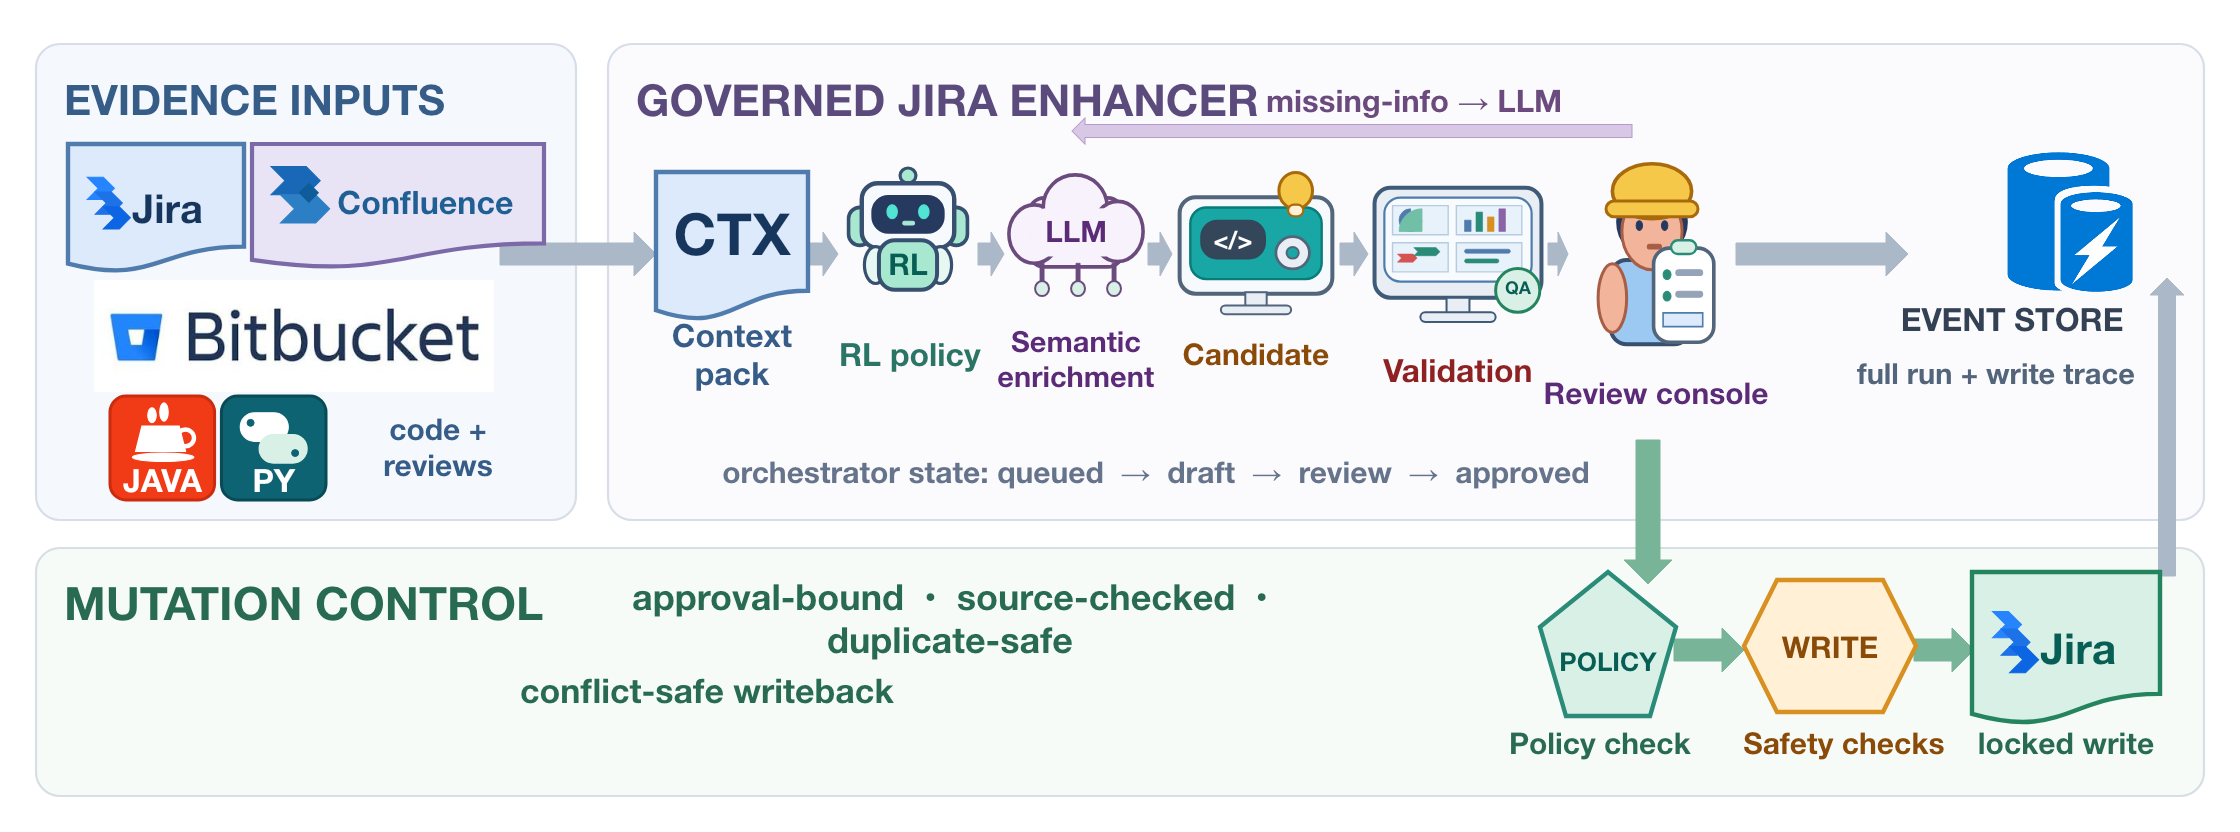
\includegraphics[width=\textwidth]{images/system_architecture_embedded.png}
\caption{Human-AI collaboration architecture. Jira, Confluence, and Bitbucket provide evidence in the form of issues, requirements, design, code, and reviews. The orchestrator controls evidence-based story creation, bounded prompt arm selection, governance checks, audit storage, and controlled writeback of Jira issues. The labels and arrows define the sequence of runtime contracts that starts from the context extraction and human actions and proceeds with scoring, policy check, approved candidate generation, and mutation.}
\Description{Architecture diagram showing Jira, Confluence, and Bitbucket feeding a Jira Enhancer platform with orchestration, semantic enrichment, prompt policy, governance, persistence, and writeback components.}
\label{fig:system-architecture}
\end{figure*}

\begin{figure*}[t]
\centering
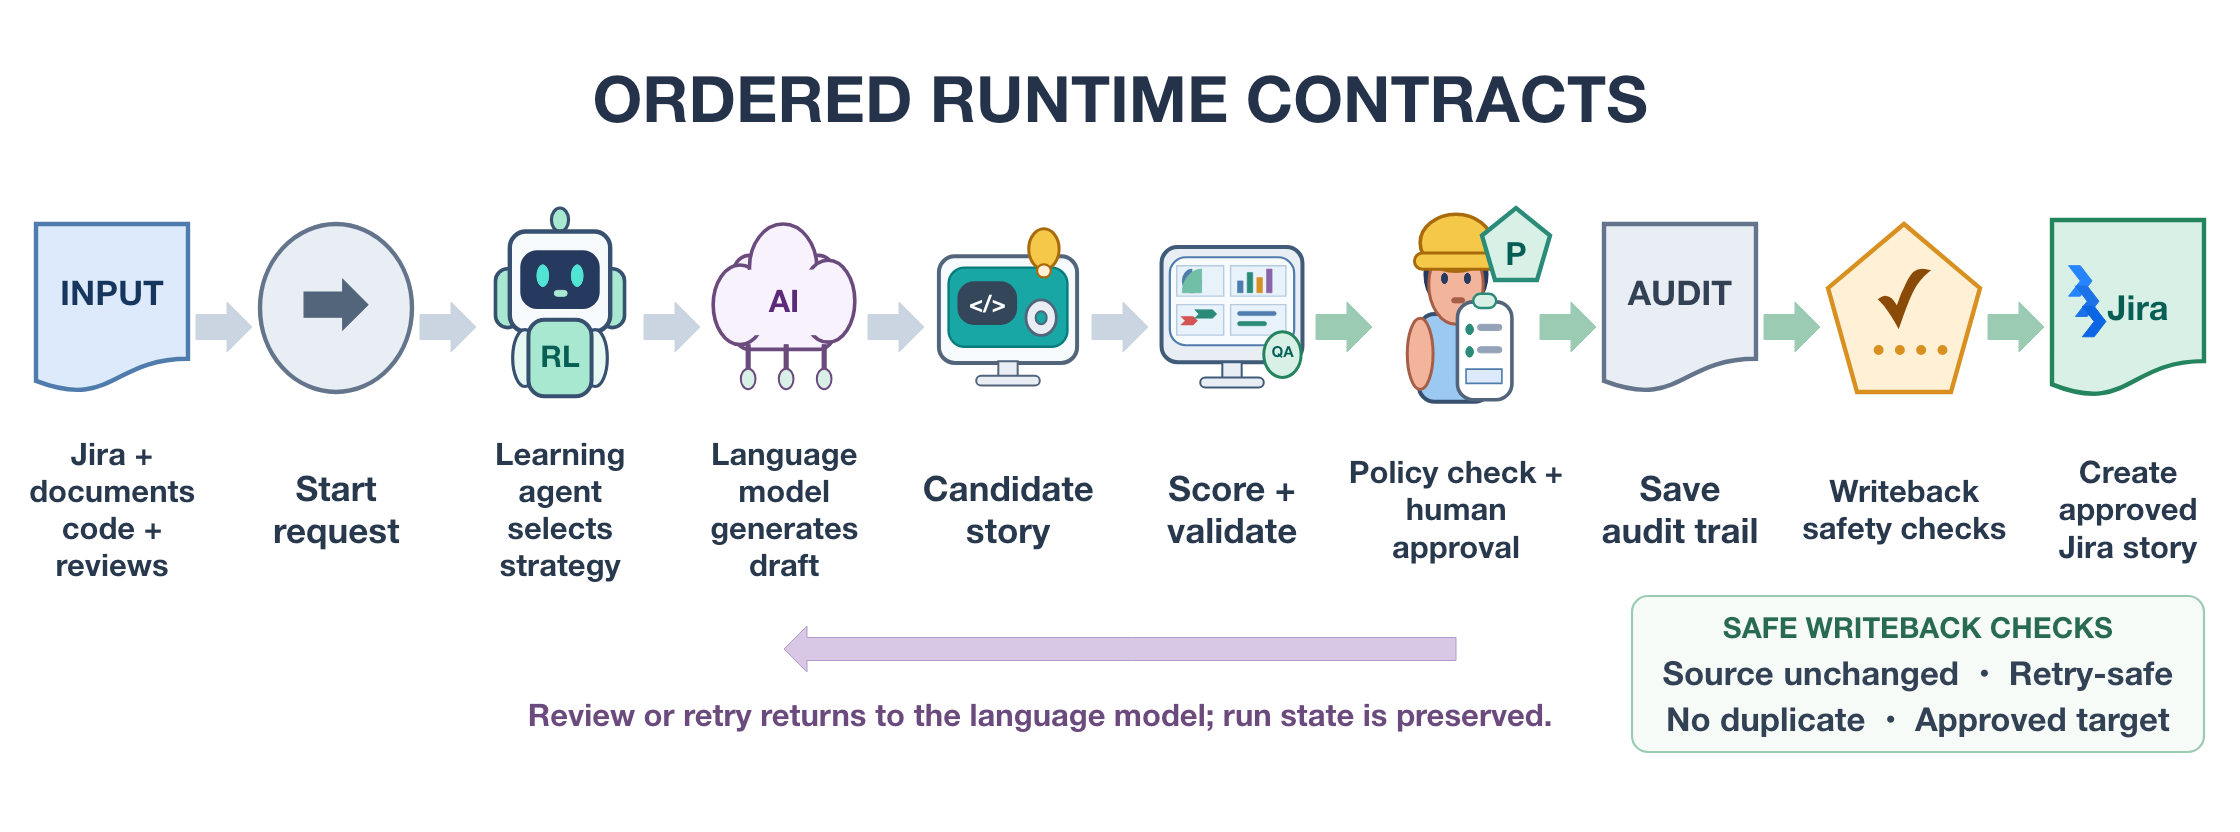
\includegraphics[width=\textwidth]{images/system_control_flow_embedded.png}
\caption{Sequence of the runtime contracts according to Fig.~\ref{fig:system-architecture}. Jira, requirements, code, and review input is fed into the orchestrator. Safe prompt selection and scoring generate the candidates, policy check and tracing storage precede the creation of approved candidates; writeback is the last step of the process.}
\Description{Control-flow diagram showing ordered handoffs from context retrieval and user action through prompt selection, draft scoring, policy decision, persistence, and approved writeback.}
\label{fig:system-control-flow}
\end{figure*}

\begin{figure*}[t]
\centering
\begin{subfigure}[t]{0.49\textwidth}
\centering
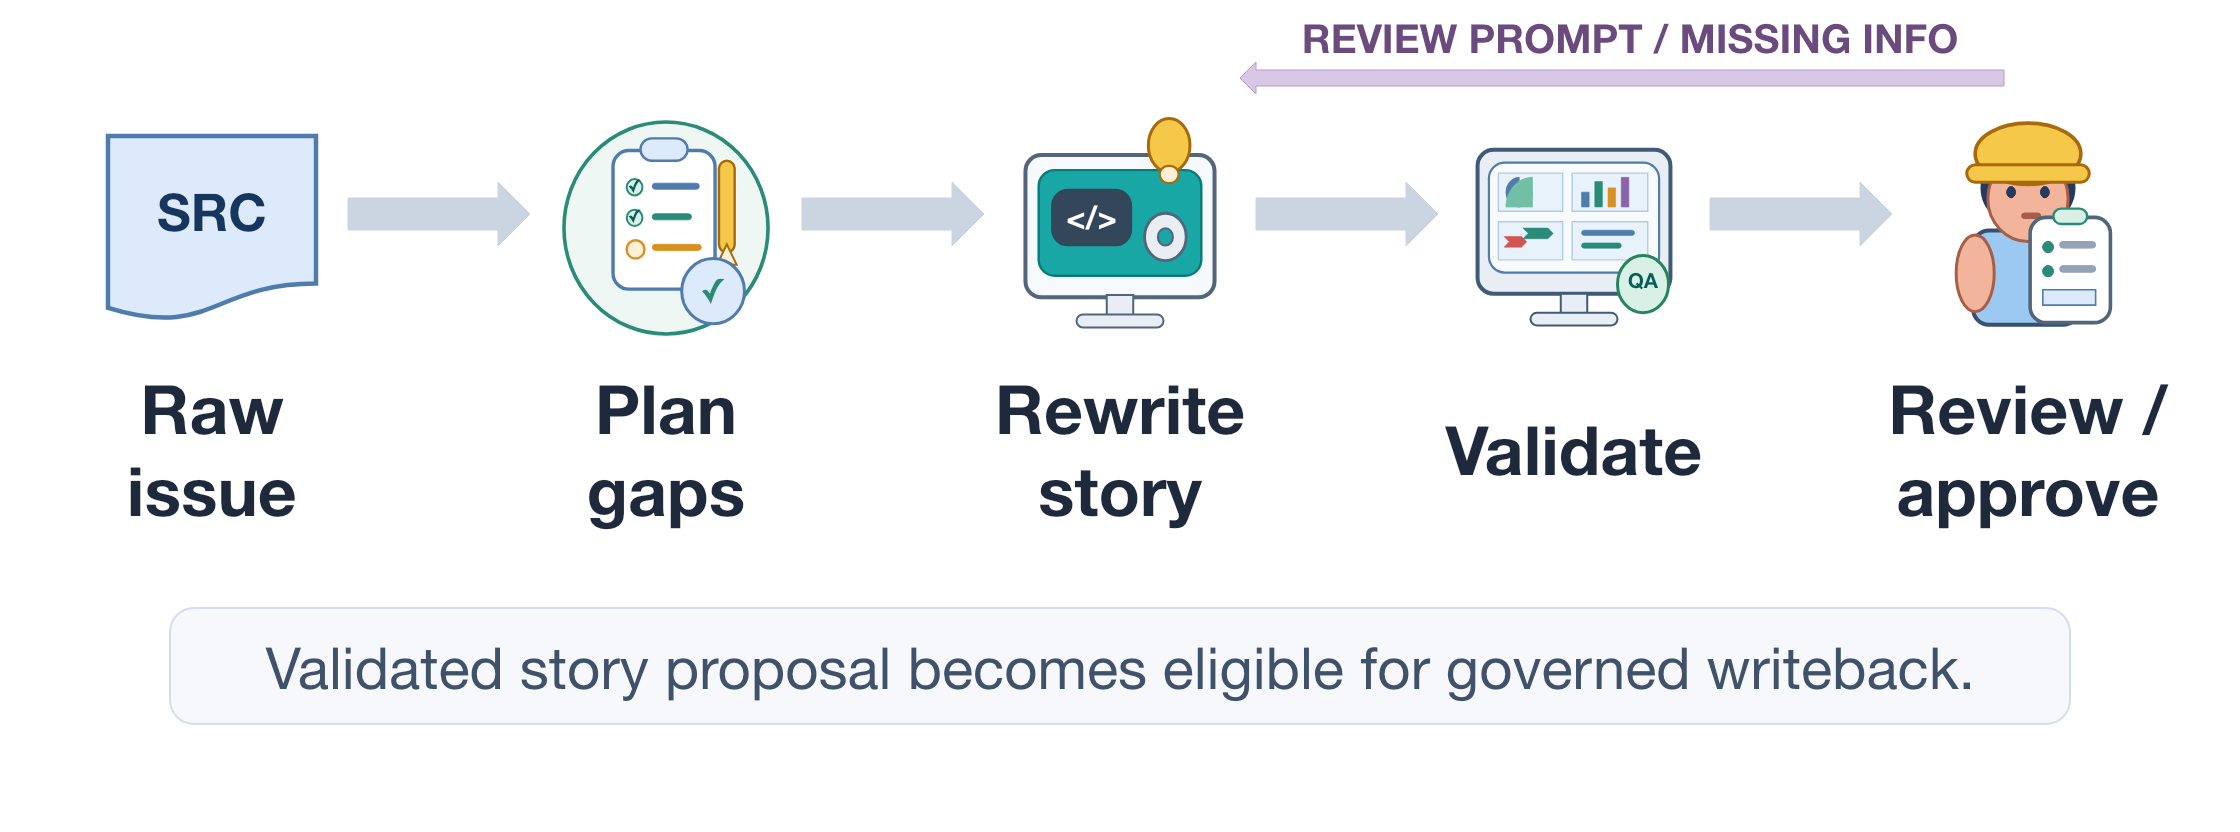
\includegraphics[width=\linewidth]{images/agentic_module_story_issue_enhancer.png}
\caption{Agentic module 1: story/issue enhancer.}
\label{fig:module-story-issue}
\end{subfigure}
\hfill
\begin{subfigure}[t]{0.49\textwidth}
\centering
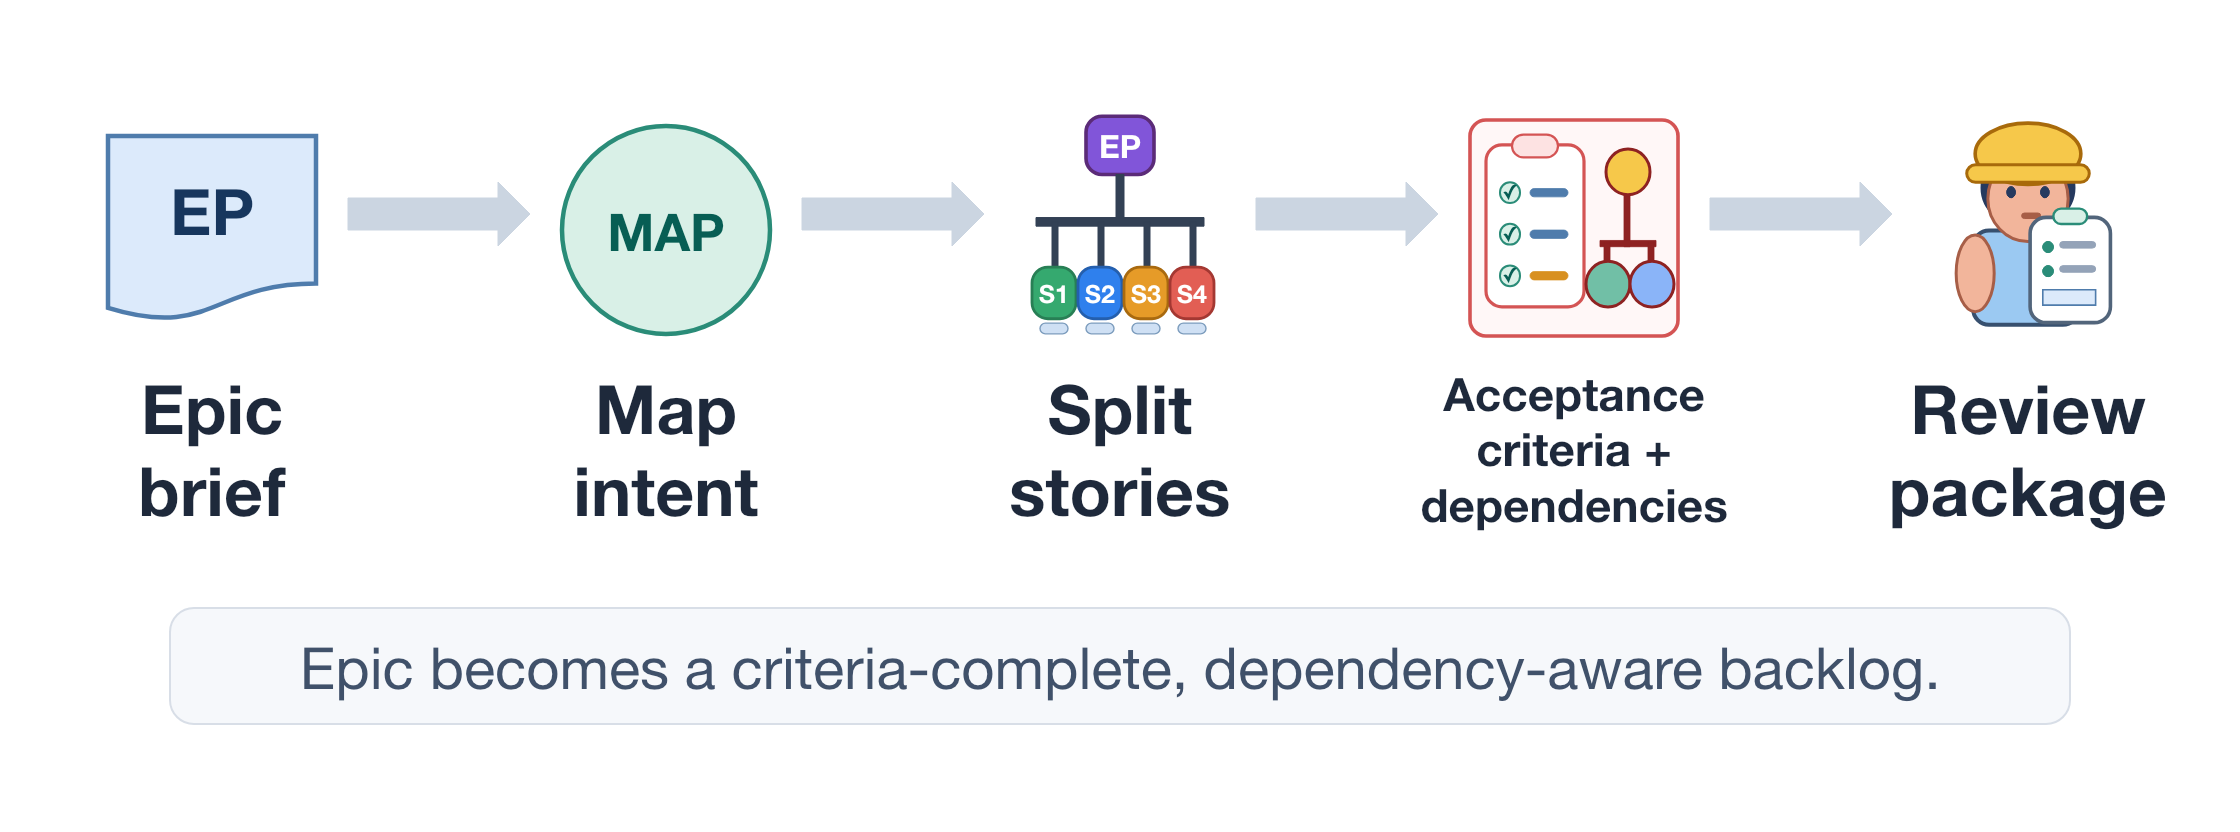
\includegraphics[width=\linewidth]{images/agentic_module_epic_breaker.png}
\caption{Agentic module 2: epic breaker into stories.}
\label{fig:module-epic-breaker}
\end{subfigure}

\vspace{0.75em}
\begin{subfigure}[t]{0.49\textwidth}
\centering
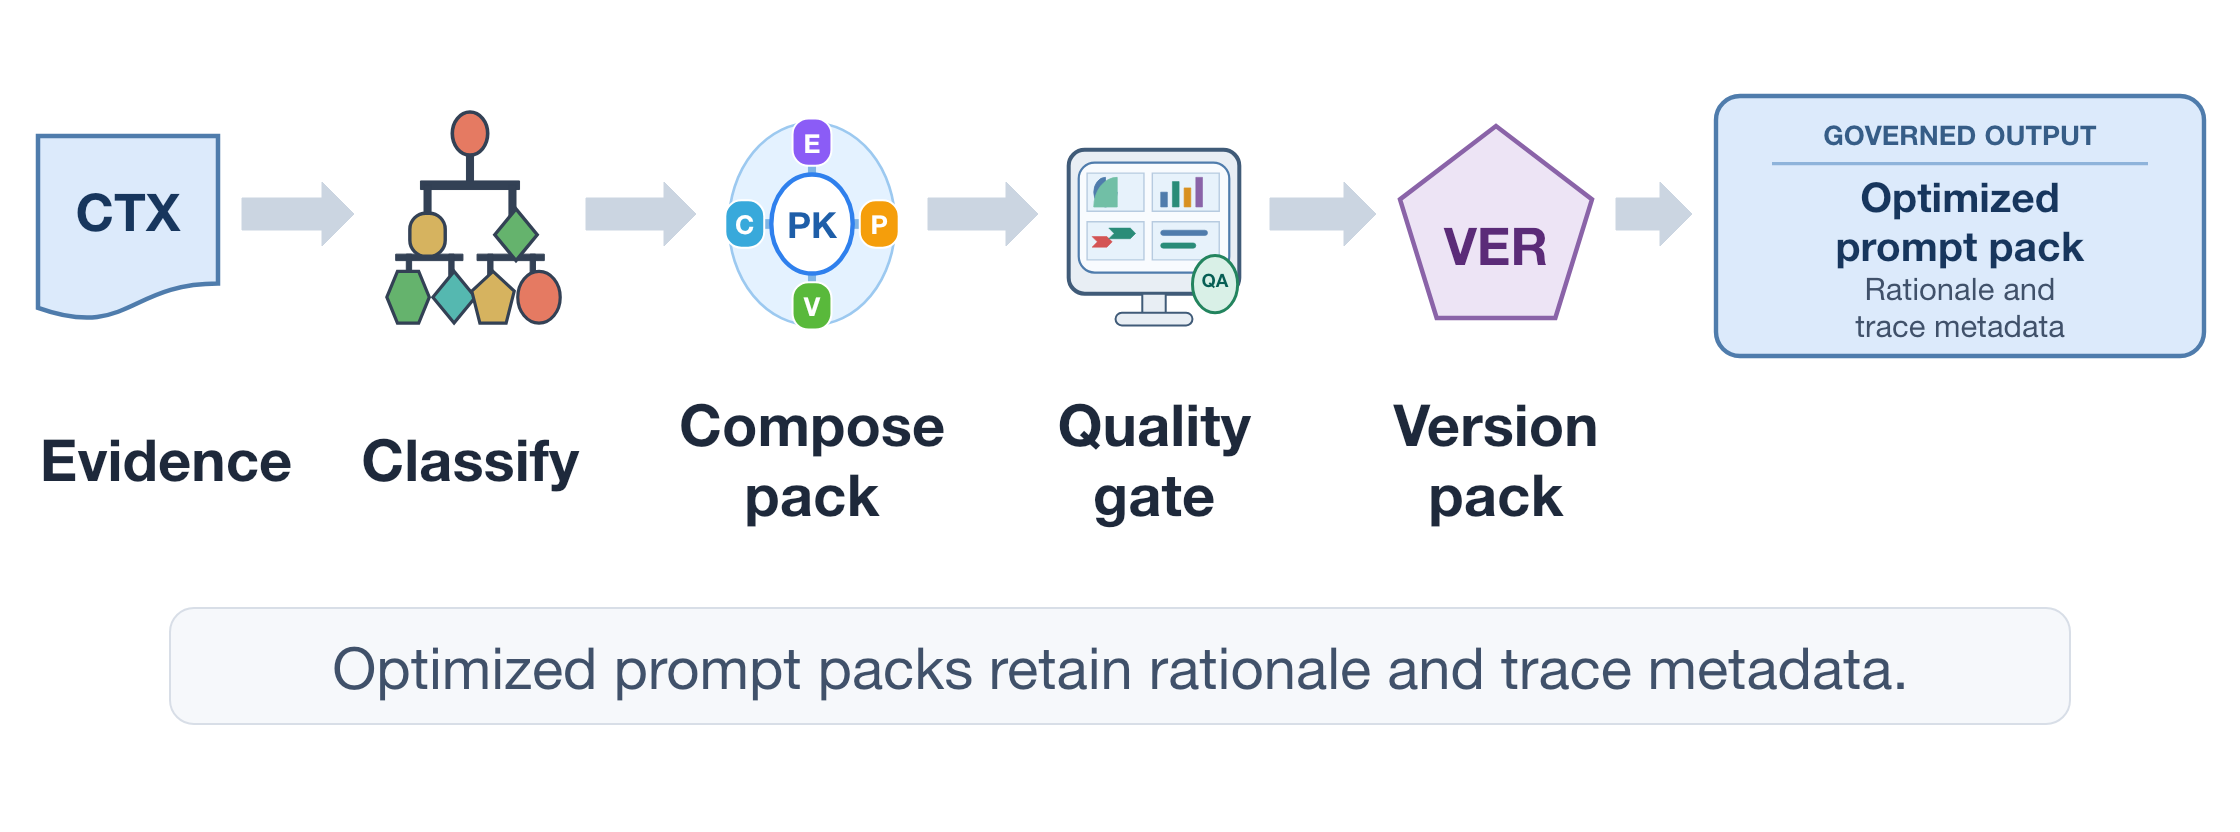
\includegraphics[width=\linewidth]{images/agentic_module_prompt_generator.png}
\caption{Agentic module 3: prompt generator.}
\label{fig:module-prompt-generator}
\end{subfigure}
\hfill
\begin{subfigure}[t]{0.49\textwidth}
\centering
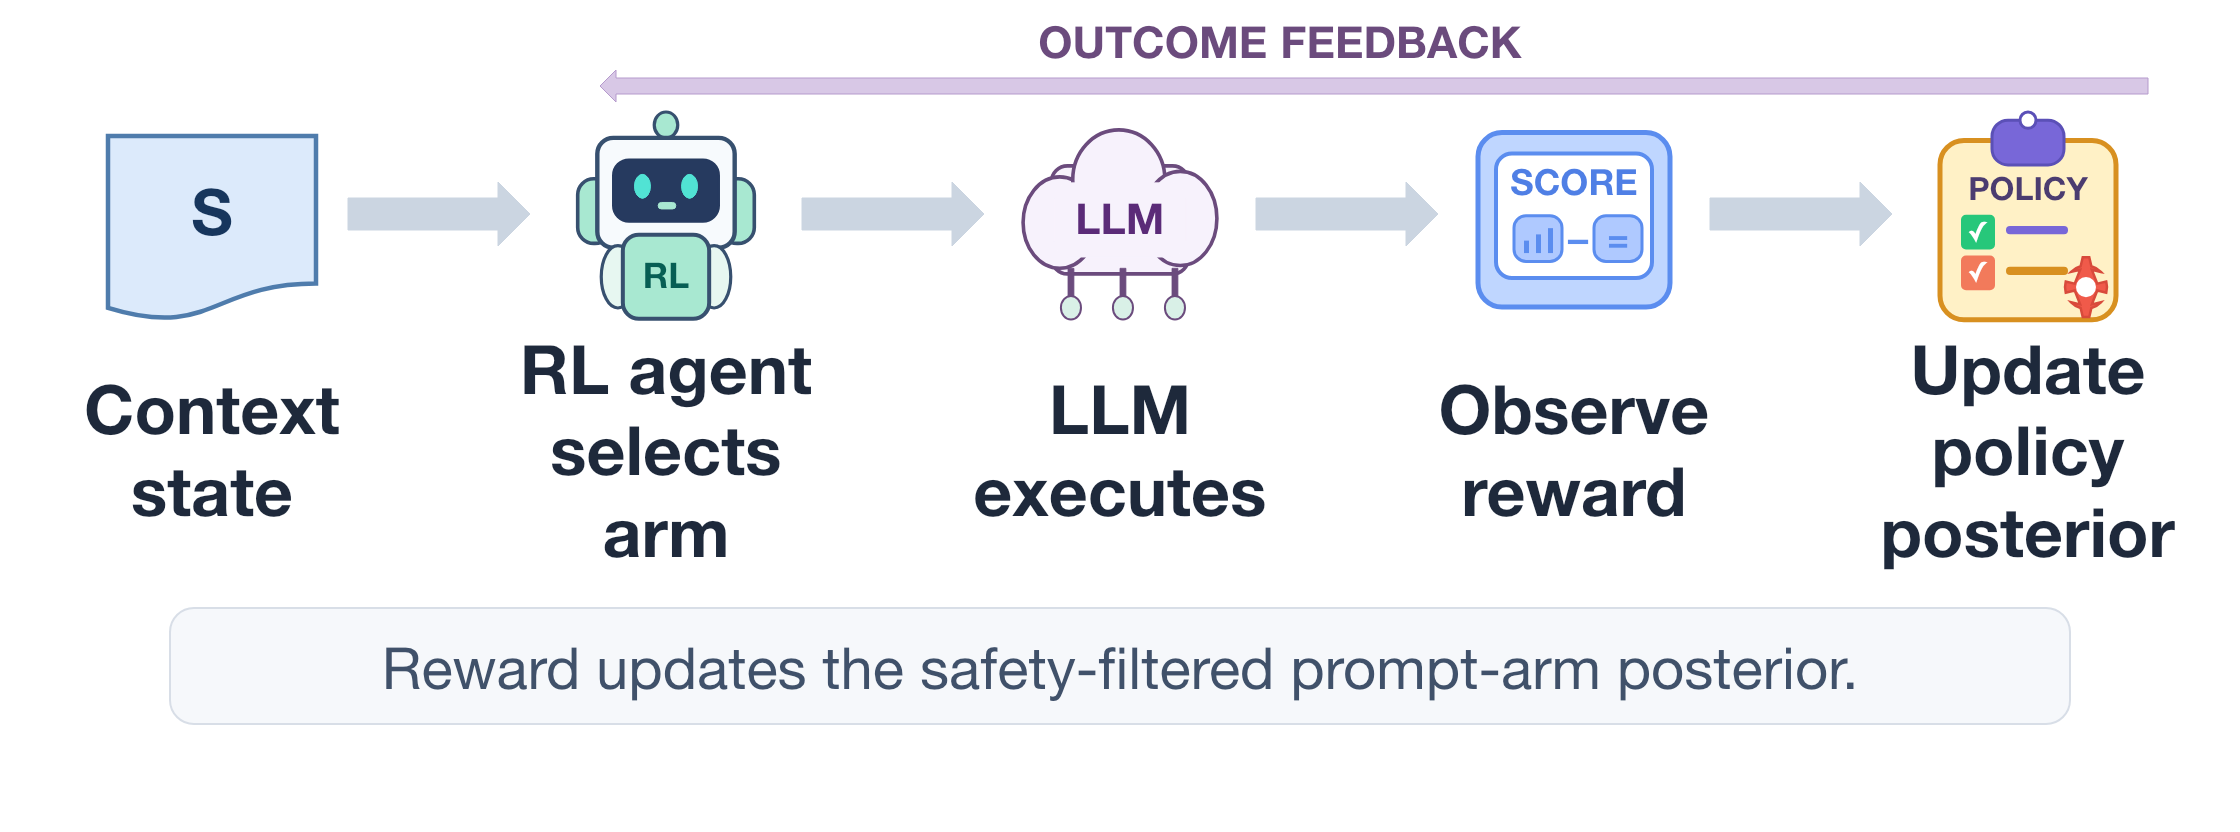
\includegraphics[width=\linewidth]{images/agentic_module_rl_controller.png}
\caption{Agentic module 4: RL controller.}
\label{fig:module-rl-controller}
\end{subfigure}
\caption{Modular agent architecture: story/issue enhancement, epic-to-story decomposition, prompt-pack creation, and RL-based policy control. The panels expose agent boundaries hidden in the top-level architecture.}
\Description{Four-panel modular architecture figure showing story issue enhancement, epic-to-story decomposition, prompt generation, and reinforcement-learning controller modules.}
\label{fig:agentic-module-architecture}
\end{figure*}

\subsubsection{Reading Figures 1--3}

The set of Figures~\ref{fig:system-architecture}--\ref{fig:agentic-module-architecture} provides three perspectives: architecture and trust boundaries, operational sequence, and internal decomposition of agents. The deliberate overlap helps to conduct separate reviews of completeness of the architecture, correctness of the execution, and responsibilities of agents.

\paragraph{Figure 1: system architecture overview.}
Figure~\ref{fig:system-architecture} places Jira epics, stories, and writeback targets; Confluence requirements and design evidence; and Bitbucket code and review signals outside the AI boundary. Inside Jira Enhancer, the review console, orchestrator, semantic enrichment engine, RL policy, governance layer, event store, and conflict-safe writer transform evidence into candidate stories. The architecture clearly separates AI reasoning from changes to Jira. The enrichment and RL components can generate, evaluate, and improve a candidate story, but they cannot update Jira directly. A candidate can be written to Jira only after it passes validation and the confidence threshold, complies with the relevant policies, and receives human approval.

\paragraph{Figure 2: execution/control flow.}
Figure~\ref{fig:system-control-flow} displays the components in execution order. A run gathers Jira context and acquires requirement, design, code, and review signals. The orchestrator first makes a workflow entry and selects a permitted prompt strategy. Then, it generates and scores candidate stories, applies the policies, and logs all the steps. Only successful candidates may be written to Jira. Each arrow in the diagram depicts a clearly defined handoff from one component to another, which includes preparing inputs, logging the selection of prompts, candidate scoring, logging the policies applied, and validation of writing back to Jira. Before writing to Jira, the system ensures there are no conflicting edits, safe retries (idempotency), and duplicated stories. Otherwise, the item is left in review, refinement, conflict, or failure state without Jira being updated.

\paragraph{Figure 3: Internal agent modules.}
Figure~\ref{fig:agentic-module-architecture} demonstrates four agentic capabilities within the AI engine. The first Agentic Module evaluates an issue and determines what acceptance criteria, testability, risks, and refinement areas are absent. The second Agentic Module creates candidate stories and dependencies for a high-level epic, adding acceptance criteria and data for human review. The third Agentic Module generates context-aware prompt packs using the issue text, reusable patterns, policy constraints, and information gaps that were identified. The fourth Agentic Module plays a role of an RL controller. It chooses an approved strategy to create prompts -- policy arm, evaluates the outcome, rewards it according to its quality, and adjusts the posterior estimate that is a measure of future success of the corresponding strategy. It enables the choice between different strategies, such as conservative decomposition and balanced-context generation, while avoiding any unsafe or unrestricted prompts.

The captions in Figures~\ref{fig:system-architecture} and~\ref{fig:system-control-flow} represent executable contracts. Context and Code Retrieve normalize the inputs, \textit{Human Actions} captures the reviewer's intention, while selecting and generating safe-arms leads to scoring of candidates; \textit{Policy Check} determines confidence, role, validation, and approval; \textit{Persist trace} records state, results, and evidence links. Approved creation reaches controlled writeback only after the source hash, idempotency, duplicate, and target checks. The safety boundary is hence determined by this rule rather than fluency of text.

\subsubsection{Traceable Data Records}
Every run captures scope, requester, time stamps, and idempotency information along with item state, confidence, readiness, policy flags, structured drafts, references to external evidence, decisions and notes on approval, and before/after writeback hashes. Since each piece of information is a first class record, the planning decision behind it may be subsequently reconstructed for empirical evaluation \cite{R54,R70}, auditing \cite{R93}, or incident analysis. Immutable event streams maintain event ordering, whereas mutable snapshots facilitate low-latency querying. Informational warnings alert about non-critical deficiencies, advisory warnings bring problems to reviewer attention, and blocking warnings stop mutation until the issue gets fixed.

\subsection{Notation and Scale Conventions}

Table~\ref{tab:notation} includes the notation used in the mathematical models and algorithms. Confidence and readiness vary in $[0,1]$ unless otherwise specified. The notation $C_{10}(s)=10C(s)$ denotes the corresponding value on the zero-to-ten scale of the interface. The creation gate is configured as $\tau_c=0.9$. We use $\tau_e$ for the escalation. Subscripts $s$, $t$, $k$, and $m$ stand for a story, refinement attempt, prompt arm, and evaluation method, respectively. In case of a base letter with engineering and statistical meanings, we qualify it with the appropriate subscript.

\begingroup
\footnotesize
\setlength{\tabcolsep}{3pt}
\setlength{\LTpre}{4pt}
\setlength{\LTpost}{4pt}
\renewcommand{\arraystretch}{0.92}
\begin{longtable}{@{}>{\raggedright\arraybackslash}p{0.31\textwidth}>{\raggedright\arraybackslash}p{0.64\textwidth}@{}}
\caption{Comprehensive notation used in the formal models, algorithms, and evaluation.}\label{tab:notation}\\
\toprule
Symbol & Definition \\
\midrule
\endfirsthead
\multicolumn{2}{c}{\tablename\ \thetable\ (continued)}\\
\toprule
Symbol & Definition \\
\midrule
\endhead
\midrule
\multicolumn{2}{r}{Continued on next page}\\
\endfoot
\bottomrule
\endlastfoot

\multicolumn{2}{@{}l}{\textbf{Planning, evidence, and constrained selection}}\\
$E, E_u$ & Epic under analysis; $E_u$ is an epic unit supplied to an evaluation core. \\
$s,s_i,s_j$ & Candidate story and indexed candidate stories. \\
$S_{\mathrm{existing}}$ & Stories already linked to $E$. \\
$S_{\mathrm{cand}}$ & Finite candidate-story set generated for $E$. \\
$S_{\mathrm{new}}$ & Candidate subset proposed for possible creation. \\
$S_{\mathrm{eligible}}$ & Duplicate-free candidates satisfying confidence, approval, validation, and policy-allow conditions. \\
$S_{\mathrm{create}}$ & Stories successfully added to the controlled creation set. \\
$S^*$ & Augmented plan $S_{\mathrm{existing}}\cup S_{\mathrm{new}}$. \\
$\mathcal{D},\mathcal{D}_{\mathrm{ext}},\mathcal{D}_{\mathrm{jira}}$ & Complete evidence corpus, externally retrieved evidence, and Jira-embedded evidence. \\
$\mathbf{m}(s)$ & Candidate metric tuple containing confidence, readiness, utility, ambiguity, risk, approval, and source hash. \\
$C(s),C_s$ & Normalized confidence in $[0,1]$ for story $s$ and its algorithmic shorthand. \\
$C_{10}(s),C_{10,t}$ & Displayed confidence for story $s$ and at refinement attempt $t$ on the zero-to-ten UI scale, with $C_{10}(s)=10C(s)$. \\
$R(s),R_s,R_s(\mathbf{x})$ & Readiness of story $s$, its algorithmic shorthand, and readiness viewed as a function of evidence coverage. \\
$U(s),\operatorname{Amb}(s),\rho(s)$ & Expected utility, ambiguity, and risk of candidate $s$. \\
$A(s),A_s$ & Explicit human-approval indicator and its algorithmic shorthand; both are binary. \\
$V(s),V_s$ & Validator result for schema, contradiction, and required-field checks; both are binary. \\
$\Pi,\Pi(s),g_{\Pi}(s)$ & Versioned governance policy, its decision for $s$, and the binary policy-allow indicator. \\
$I_{\mathrm{ctx}}(s)$ & Binary indicator that story $s$ is operating with limited external context. \\
$I_{\mathrm{esc}}(s),I_{\mathrm{create}}(s)$ & Binary escalation-required and creation-eligibility predicates for story $s$. \\
$h_s,H(\cdot)$ & Source-state hash stored at decision time and deterministic cryptographic hash function. \\
$\tau_c,\tau_{10},\tau_e,\tau_r$ & Normalized creation threshold (default $0.9$), its displayed equivalent $\tau_{10}=10\tau_c$, escalation threshold, and offline replay shaping threshold ($0.8$). \\
$y_s$ & Binary selection variable; $y_s=1$ selects $s$ for the augmented plan. \\
$\mathbb{1}[\cdot]$ & Indicator function, equal to one when its predicate is true and zero otherwise. \\
$\operatorname{summary}(s),\operatorname{norm}(\cdot)$ & Story summary and deterministic lowercase/alphanumeric normalization. \\
$\sim_n,\mathcal{F}_{\mathrm{dup}}$ & Normalized-summary equivalence relation and duplicate-free candidate domain. \\
$\lambda_{\rho},\lambda_{\mathrm{Amb}}$ & Non-negative objective weights for risk and ambiguity. \\
$\mathrm{SP}(s),B_{\mathrm{sprint}}$ & Story-point estimate for candidate $s$ and sprint story-point budget. \\
$\operatorname{dep}(s_i,s_j),\operatorname{team}(s),g,\operatorname{cap}_g,\operatorname{ord}(s)$ & Dependency indicator, assigned team, team index, team-capacity bound, and release-order position. \\
$f(\cdot),\xi_{\mathrm{scope}},\xi_{\mathrm{integration}},\xi_{\mathrm{risk}},\xi_{\mathrm{unknown}}$ & Story-point mapping and normalized complexity priors were used for the initial assignment. \\
$\mathcal{W}_{\mathrm{create}}$ & Result of the controlled creation operation on $S_{\mathrm{eligible}}$. \\

\addlinespace[2pt]
\multicolumn{2}{@{}l}{\textbf{Readiness, confidence, and calibration}}\\
$\mathbf{x}=(x_d,x_a,x_p,x_e,x_h,x_g)$ & Binary vector of evidence for the description, acceptance criteria, dependencies, external evidence, activity history, and edge cases. \\
$R_{\mathrm{src}}(\mathbf{x})$ & Base evidence score computed as a weighted sum of the evidence coverage vector $\mathbf{x}$. \\
$B_{\mathrm{gen}},P_{\mathrm{gap}}$ & Bounded generated-content bonus and evidence-gap penalty. \\
$z_i,w_i,b_{\max}$ & The quality facet of the generated content and the weight of the facet; the bounded generated bonus total. \\
$\eta_d,\eta_a,\eta_p,\eta_e$ & Gap-penalty weights (non-negative) for missing description, acceptance criteria, dependencies, and external evidence. \\
$\delta_C,\gamma_{\mathrm{ceiling}}$ & Bounded confidence update and the evidence-based confidence ceiling. \\
$\operatorname{clip}(u,a,b)$ & Clipping operator $\min(\max(u,a),b)$. \\
$\operatorname{ECE},\operatorname{Brier}$ & Expected calibration error and Brier score; both require post-delivery labels. \\

\addlinespace[2pt]
\multicolumn{2}{@{}l}{\textbf{Prompt policy, reward, and convergence}}\\
$p_k,k$ & Prompt pack associated with arm $k$ and the arm index. \\
$\theta_k,\widetilde\theta_{k,t}$ & Success probability of the underlying arm and its Thompson sample at attempt $t$. \\
$\alpha_k,\beta_k$ & Soft counts of successes and failures for the Beta posterior of arm $k$. \\
$n_k,\bar r_k$ & Number of recorded outcomes and running mean reward for arm $k$. \\
$\mathbf{h}_t$ & Context feature state used for choosing the policy at attempt $t$. \\
$\mathcal{K},\mathcal{K}_{\mathrm{safe}}(\mathbf{h}_t)$ & Complete set of prompt arms and the subset that satisfies every governance condition at attempt $t$. \\
$\chi_j(k,\mathbf{h}_t)$ & Binary governance check for arm $k$ under condition $j$ and context $\mathbf{h}_t$; 1 means satisfied and 0 means rejected. \\
$j,n_{\chi}$ & Governance-condition index and total number of governance conditions. \\
$C^{\mathrm{before}}_{10,t},C^{\mathrm{after}}_{10,t}$ & Displayed confidence before and after the recorded outcome for selected arm $k_t$. \\
$d_t,w_t$ & Recorded reviewer decision and writeback status for the selected arm. \\
$r_t,q_t$ & Signed reward clipped to $[-1,1]$ and its fractional Beta success credit $q_t=(r_t+1)/2$. \\
$T,t,k_t$ & Horizon of attempts, attempt number, and arm chosen at attempt $t$. \\
$\ell_t,\ell_0,\ell(t),\ell(0)$ & Confidence gap at attempt $t$, its algorithmic initial value, its continuous interpolation, and the corresponding continuous-time initial gap. \\
$\kappa,\widehat\kappa_t$ & Effective lag-convergence rate and its attempt-level estimate. \\
$d_{\ell}(t),d_{\max}$ & Lag disturbance and its assumed absolute bound. \\
$\mathbb{E}[\cdot],\Pr(\cdot),\arg\max$ & Expectation, probability, and maximizing-argument operators. \\
$\mathcal{L}\{\cdot\},s_L,\Lambda_{\ell}(s_L),D_{\ell}(s_L)$ & Laplace-transform operator, Laplace-domain variable, transform of $\ell(t)$, and transform of $d_{\ell}(t)$. \\
$\epsilon$ & Positive numerical guard for rate estimation. \\
$\mathcal{X},\mathcal{P},\mathcal{C},\mathcal{T}_{\mathrm{audit}}$ & Connector set, prompt-policy state, retrieved context pack, and durable attempt/audit trace. \\

\addlinespace[2pt]
\multicolumn{2}{@{}l}{\textbf{Approval-bound mutation and batch outcomes}}\\
$\mathcal{E}_a,\mathcal{E}_t$ & Approved source-bound transaction envelope and the corresponding runtime envelope evaluated immediately before mutation. \\
$r_{\mathrm{run}},i_{\mathrm{issue}}$ & Run and issue identifiers bound into $\mathcal{E}_a$. \\
$\nu_s,\nu_d,h_d$ & Approved source revision, draft version, and draft payload hash; the approved source hash is $h_s$. \\
$\nu_{\Pi},h_{\Pi}$ & Approved governance-policy version and policy-snapshot hash. \\
$\mathcal{T}_{\mathrm{target}}$ & Canonical set of allowed mutation targets. \\
$a_{\mathrm{dec}},u_{\mathrm{rev}},t_a$ & Approval decision, reviewer identifier, and approval time. \\
$I_{\mathrm{tx}}$ & Transaction identifier $H(\mathcal{E}_a)$. \\
$K_{A2},K_{A3}$ & A2 payload-level idempotency key and A3 source-bound envelope key. \\
$\mathrm{A0},\mathrm{A1},\mathrm{A2},\mathrm{A3}$ & Mutation-safety arrangements: ordinary approval/logging, source-hash conditional write, source hash with atomic idempotency, and the source-bound transaction envelope. \\
$h_{\mathrm{current}},h_{\mathrm{expected}}$ & Runtime source hash and approved source hash expected by writeback, where $h_{\mathrm{expected}}:=h_s$. \\
$\operatorname{permit}(\mathcal{E}_a,\mathcal{E}_t)$ & Binary mutation authorization predicate. \\
$\operatorname{write}(s)$ & Binary write indicator; it equals one when story $s$ is written to Jira and zero otherwise. \\
$o_s,\mathcal{B}_{\mathrm{batch}},\operatorname{status}(\mathcal{B}_{\mathrm{batch}})$ & Per-story creation outcome, candidate batch, and precedence-derived batch status. \\

\addlinespace[2pt]
\multicolumn{2}{@{}l}{\textbf{Evaluation and statistical analysis}}\\
$\mathrm{B0},\mathrm{B1},\mathrm{B2},\mathrm{B3},m$ & Manual reference, template/rule core, one-shot drafting control, Jira Enhancer, and method index. \\
$Q_m,\mathrm{Eff}_m,G_m,\mathrm{Composite}_m,\mathrm{Time}_m$ & Quality, efficiency, governance, composite, and time indices for method $m$. \\
$w_Q,w_{\mathrm{Eff}},w_G$ & Fixed non-negative composite-index weights that sum to one. \\
$\Delta$ & Formula-derived composite difference to B3 within an input set. \\
$Q_{\mathrm{omni}}$ & Matched-study permutation omnibus statistic. \\
$r_{rb}$ & Paired rank-biserial effect size. \\
$n,\mathrm{SD},\mathrm{IQR},\mathrm{P90}$ & Generic sample size, sample standard deviation, interquartile range, and 90th percentile. \\
$p,p_{\mathrm{Holm}}$ & Raw or Holm-adjusted probability value. \\
$\mathrm{CI},\mathrm{ICC}(2,1)$ & Confidence interval and two-way random-effects absolute-agreement intraclass correlation. \\
$\texttt{service\_mode}$ & Connector operating mode: \texttt{full-context} or \texttt{reduced-context}. \\
\end{longtable}
\endgroup


\subsection{Formal Problem Formulation}

Let $E$ be an epic, $S_{\text{existing}}$ the set of already-linked stories, $\mathcal{D}$ the available evidence corpus, and $\Pi$ a versioned governance policy. The evidence corpus is decomposed as $\mathcal{D}=\mathcal{D}_{\mathrm{ext}}\cup\mathcal{D}_{\mathrm{jira}}$, where $\mathcal{D}_{\mathrm{ext}}$ contains external evidence from Confluence/Bitbucket and $\mathcal{D}_{\mathrm{jira}}$ contains embedded design context in the Jira description. This distinction is important because, when external links are unavailable but the epic description contains useful design rules, APIs, guardrails, or tests, the system can still produce evidence-grounded candidates while identifying their provenance as Jira-embedded context. The system constructs a finite candidate set $S_{\text{cand}}$ and selects a subset $S_{\text{new}}\subseteq S_{\text{cand}}$ for possible creation. Here, requirements are modeled as evolving and negotiated objects rather than fixed text \cite{R51}. This agrees with established RE views that requirements are incomplete and shaped by stakeholders \cite{R61}. It also follows requirements-quality guidance on clarity, verifiability, feasibility, and traceability \cite{R62}. Each candidate $s$ is represented by the tuple
\begin{equation}
\mathbf{m}(s)=\left(C(s),R(s),U(s),\operatorname{Amb}(s),\rho(s),A(s),h_s\right),
\end{equation}
where $C(s)$ denotes normalized confidence, $R(s)$ denotes readiness, $U(s)$ is expected utility, $\operatorname{Amb}(s)$ is ambiguity, $\rho(s)$ is risk, $A(s)\in\{0, 1\}$ is human approval, and $h_s$ is the source-state hash when decision is made.

Normalized story identity is modeled through an equivalence relation $\sim_n$:
\begin{equation}
s_i \sim_n s_j \iff \operatorname{norm}(\operatorname{summary}(s_i)) =
\operatorname{norm}(\operatorname{summary}(s_j)),
\end{equation}
Norm works by converting text to lowercase and stripping all non-alphanumeric separators from it. The duplicate-free candidate domain is thus:
\begin{equation}
\mathcal{F}_{\mathrm{dup}}=\{s\in S_{\text{cand}}\mid \nexists s'\in S_{\text{existing}}: s\sim_n s'\}.
\end{equation}
The above guarantees that work item generation will not lead to duplicates caused by normalization, which would make different versions of task summaries identical.

The basic feasibility relation is:
\begin{align}
S^* &= S_{\text{existing}} \cup S_{\text{new}}, \\
\forall s \in S_{\text{new}}:~ C(s) &\geq \tau_c, \\
\forall s \in S_{\text{new}}:~ A(s) &= 1 \text{ (approved)}, \\
S_{\text{eligible}} &= \{ s \in S_{\text{new}}\cap\mathcal{F}_{\mathrm{dup}} \mid C(s)\ge \tau_c \land A(s)=1 \land V(s)=1 \land \Pi(s)=\textsc{allow} \}, \\
\mathcal{W}_{\text{create}} &= \text{Create}(S_{\text{eligible}}),
\end{align}
where $\tau_c\in[0,1]$ is the normalized creation threshold (default $\tau_c=0.9$, displayed as $C_{10}(s)=9$, i.e., 9/10), and
$V(s)\in\{0,1\}$ is the validation indicator for candidate story $s$.
It holds true (i.e. 1) only if the candidate passes schema, contradiction, and required field test. Condition $\Pi(s)=\textsc{allow}$ represents that the governing policy of the machine allows creation of the candidate.

This expression contains one of the important principles: high quality of generation does not necessarily guarantee the mutation. Creation is an action demanding both trust of the machine and of the human being, so that recommendation cannot become an action without permission.

Feasibility rules defined above specify which candidates are eligible for the creation phase. Yet, several of the candidates will satisfy all those rules and the machine still needs to determine which of them must enter the enhanced plan.

For each of the candidates $s\in S_{\text{cand}}$, we will define a binary decision variable $y_s\in\{0,1\}$, where $y_s=1$ if the candidate is selected and $y_s=0$ if it is not selected. The system uses the following objective:
\begin{equation}
	\max_{\{y_s\}} ~ \sum_{s \in S_{\text{cand}}} y_s
	\Big(
	U(s)-\lambda_\rho\rho(s)
	-\lambda_{\mathrm{Amb}}\operatorname{Amb}(s)
	\Big),
\end{equation}
subject to:
\begin{align}
	y_s &\leq \mathbb{1}[C(s)\ge \tau_c], \\
	y_s &\leq A(s), \\
	y_s &\leq V(s), \\
	y_s &\leq \mathbb{1}[\Pi(s)=\textsc{allow}], \\
	y_s &\leq 1-\mathbb{1}[\exists s'\in S_{\text{existing}}:
	\operatorname{norm}(\operatorname{summary}(s))
	=
	\operatorname{norm}(\operatorname{summary}(s'))], \\
	y_s &\in \{0,1\}.
\end{align}

Objective favours candidates with high expected utility $U(s)$. Selection score decreases if the candidate has high risk $\rho(s)$ or high ambiguity $\operatorname{Amb}(s)$. Non-negative weights $\lambda_\rho$ and $\lambda_{\mathrm{Amb}}$ define the degree to which risk and ambiguity influence selection.

Constraints make it possible to select a candidate only when its confidence level equals $\tau_c$, it has human approval, it has passed validation, and active policy allows for its creation. The duplicate constraint makes it impossible to select a candidate whose normalized summary coincides with an existing story. In this case, $\mathbb{1}[\cdot]$ equals one if the condition is met and zero otherwise, whereas $\operatorname{norm}(\cdot)$ does deterministic summary normalization.

Thus, expected utility makes it possible to rank suitable candidates but cannot overcome confidence, approval, validation, policy, or duplicate conditions.

In scheduling applications, the objective can be extended with portfolio constraints:
\begin{align}
\sum_{s \in S_{\text{cand}}} y_s\,\mathrm{SP}(s) &\leq B_{\text{sprint}}, \\
\sum_{s \in S_{\text{cand}}} y_s\,\mathbb{1}[\operatorname{team}(s)=g] &\leq \operatorname{cap}_g, \\
\operatorname{dep}(s_i,s_j)=1 &\Rightarrow \operatorname{ord}(s_i) < \operatorname{ord}(s_j),
\end{align}
where $\mathrm{SP}(s)$ is the story-point estimate for candidate $s$, $B_{\text{sprint}}$ is the sprint budget, $\operatorname{cap}_g$ is the capacity bound for team $g$, and $\operatorname{ord}(\cdot)$ is a release-ordering function. This demonstrates that the proposed mechanism can support both decomposition quality and downstream planning feasibility.

Two invariants follow directly from the constraints:
\begin{align}
y_s=1 &\Rightarrow C(s)\ge\tau_c, \\
y_s=1 &\Rightarrow A(s)=1 \land V(s)=1 \land \Pi(s)=\textsc{allow}.
\end{align}
Consequently, selected stories are both confidence-feasible and governance-feasible. These invariants support the multi-gate creation rule used later in the policy layer.
\paragraph{Proposition 1: eligibility soundness.}
For any candidate $s\in S_{\text{cand}}$, if $y_s=1$ in the constrained optimization problem above, then $s$ is confidence-feasible, approval-feasible, validation-feasible, policy-feasible, and duplicate-free:
\begin{equation}
y_s=1 \Rightarrow
C(s)\ge\tau_c \land A(s)=1 \land V(s)=1 \land \Pi(s)=\textsc{allow} \land s\in\mathcal{F}_{\mathrm{dup}}.
\end{equation}
\textit{Proof sketch.}
The implication follows by substituting $y_s=1$ into all five eligibility upper-bound constraints. Because $y_s$ is binary, every upper bound must evaluate to one; otherwise, the corresponding constraint would be violated. Hence, the confidence, approval, validation, policy, and duplicate constraints hold simultaneously.

\paragraph{Proposition 2: Mutation Requires Approval.}
If $A(s)=0$, then $s$ cannot be selected for creation under the optimization model:
\begin{equation}
A(s)=0 \Rightarrow y_s=0.
\end{equation}
\textit{Proof sketch.}
Approval condition says $y_s\le A(s)$. Given $A(s)=0$ and $y_s\in\{0,1\}$, the only feasible value is $y_s=0$. It establishes the human-authority invariant.

The system is set up for use in cases where confidence and approval will be the main factors involved, rather than label associated with the generated output.

\subsection{Readiness and Confidence Model}
\label{sec:readiness-confidence-model}

The system calculates readiness and confidence in four steps. It first records which evidence is available. It then calculates a base evidence score, adds a bounded contribution from generated content, and subtracts penalties for missing evidence. Finally, it converts the resulting readiness score into a confidence value.

Let $\mathbf{x}\in\{0,1\}^6$ represent the available evidence:
\begin{align}
	x_d &= \mathbb{1}[\text{description exists}], \\
	x_a &= \mathbb{1}[\text{acceptance criteria exist}], \\
	x_p &= \mathbb{1}[\text{dependencies exist}], \\
	x_e &= \mathbb{1}[\text{external evidence available}], \\
	x_h &= \mathbb{1}[\text{activity history available}], \\
	x_g &= \mathbb{1}[\text{edge cases available}].
\end{align}
Each indicator equals one when the corresponding evidence is available and zero when it is missing.

The system uses these indicators to calculate the base evidence score:
\begin{equation}
	\begin{aligned}
		R_{\text{src}}(\mathbf{x}) ={}& 0.25x_d + 0.25x_a + 0.15x_p \\
		&+ 0.15x_e + 0.10x_h + 0.10x_g.
	\end{aligned}
\end{equation}
The weights are positive values and add up to one. Therefore, $R_{\text{src}}(\mathbf{x})$ remains within $[0,1]$. The description and acceptance criteria have the highest weights since they provide the most crucial information required to evaluate the candidate story.

In create-run mode, the system can apply the bounded bonus for the useful generated content:
\begin{equation}
	B_{\text{gen}}=\sum_i w_i z_i,
\end{equation}
where $z_i\in[0,1]$ denotes a quality aspect of the generated text, like the problem statement, acceptance criteria, risk model, or non-functional requirements. The weights of all these aspects satisfy $w_i\geq0$, and the sum of the weights satisfies $\sum_i w_i\leq b_{\max}$. This upper limit will prevent excessive bonuses being applied to the generated text without supportive evidence.

The system imposes penalties for the important pieces of missing evidence:
\begin{equation}
	\begin{aligned}
		P_{\text{gap}} ={}& \eta_d(1-x_d)+\eta_a(1-x_a) \\
		&+\eta_p(1-x_p)+\eta_e(1-x_e)+\cdots .
	\end{aligned}
\end{equation}
Here, the non-negative coefficients $\eta_d$, $\eta_a$, $\eta_p$, and $\eta_e$ define the penalty for the missing evidence of different types. The rest of the terms will be similar for other missing evidence.

The system calculates the readiness by combining the base score, bonus for the generated content, and penalty for the missing evidence:
\begin{align}
	R(s) &= \operatorname{clip}
	\bigl(R_{\text{src}}(\mathbf{x})+B_{\text{gen}}-P_{\text{gap}},0,0.99\bigr), \\
	C(s) &= \operatorname{clip}
	\bigl(R(s)+\delta_C,0,\gamma_{\text{ceiling}}\bigr).
\end{align}
In this case, the expression $\operatorname{clip}(u,a,b)=\min(\max(u,a),b)$ restricts a variable to be within the bounds $a$ and $b$. The expression $\delta_C$ represents a bounded confidence modification. The graphical user interface shows the confidence as $C_{10}(s)=10C(s)$ and truncates it. The maximum value that the evidence-based parameter $\gamma_{\text{ceiling}}$ can take is 1 to avoid assigning high confidence when there is not enough evidence, even if the draft is coherent.

In order to see the effect of evidence on readiness, we can also use the notation $R_s(\mathbf{x})$. If the bonus and penalty are constant, adding more evidence cannot decrease the readiness measure. Therefore,
\begin{equation}
	\mathbf{x}'\geq\mathbf{x}
	\quad\Rightarrow\quad
	R_s(\mathbf{x}')\geq R_s(\mathbf{x}),
\end{equation}
where $\mathbf{x}'\geq\mathbf{x}$ means that every evidence indicator in $\mathbf{x}'$ is equal to or greater than the corresponding indicator in $\mathbf{x}$.

\paragraph{Lemma 1: confidence is bounded.}
For any generated candidate $s$, $R(s)\in[0,0.99]$ and $C(s)\in[0,\gamma_{\text{ceiling}}]$.
\textit{Proof sketch.}
Both values are calculated using a clipping operator. By definition, $\operatorname{clip}(u,a,b)$ belongs to $[a,b]$. Thus, $R(s)$ lies in $[0,0.99]$ and $C(s)$ lies in $[0,\gamma_{\text{ceiling}}]$, irrespective of the raw evidence score, generated bonus, or gap penalty.

\paragraph{Lemma 2: monotonicity under fixed penalties.}
For $\mathbf{x}',\mathbf{x}\in\{0,1\}^6$ such that $\mathbf{x}'\ge\mathbf{x}$ componentwise, $R_s(\mathbf{x}')\ge R_s(\mathbf{x})$ if $B_{\text{gen}}$, $P_{\text{gap}}$, and $\gamma_{\text{ceiling}}$ are fixed.
\textit{Proof sketch.}
The evidence score is calculated as a non-negative weighted sum over $\mathbf{x}$, with all weights being non-negative. Hence, $R_{\text{src}}(\mathbf{x}')\ge R_{\text{src}}(\mathbf{x})$. Applying the same generated bonus and penalty, followed by a monotone clipping function, maintains this inequality.

In practice, the blended formalism shows reviewers how the confidence score was calculated. This allows them to understand whether a particular score is low because of missing acceptance criteria, insufficient evidence, or complex dependencies.

\paragraph{Confidence scope.}
In this study, confidence is a bounded decision-support score based on the available evidence. It is not a probability of successful delivery. External mutation still requires validation, policy checks, and explicit human approval. Human approval remains the final authorization decision. Therefore, the study does not use confidence to authorize mutation by itself and does not evaluate probabilistic calibration.

Additionally, the model accounts for context-dependent penalties. For example, unresolved architectural dependencies add an uncertainty term to $P_{\text{gap}}$ even when the corresponding fields are populated. This approach helps avoid high confidence for tickets that appear complete but remain semantically weak, a concern reported in agile requirements, requirements-smell, and issue-report quality research \cite{R65,R52,R53}.

\subsection{RL Prompt Selection Model}

The adaptive component in use is a contextual multi-armed bandit \cite{R86}. This can be viewed as a restricted short-horizon reinforcement-learning setting, but it does not model a long-horizon Markov decision process or estimate a value function over the workflow state space. We nevertheless refer to it as the \emph{RL layer} because that term is used in the implementation and architecture, while its learning scope remains limited.

\subsubsection{Bandit Definition}
Each $p_k$ prompt will be an arm in the stochastic multi-armed bandit \cite{R84}. Posterior per arm is:
\begin{equation}
\theta_k \sim \text{Beta}(\alpha_k, \beta_k).
\end{equation}

At each attempt $t$ \cite{R85}:
\begin{enumerate}
  \item sample $\widetilde{\theta}_{k,t}$ from the posterior of each arm in $\mathcal{K}_{\mathrm{safe}}(\mathbf{h}_t)$,
  \item choose $k_t = \arg\max_{k\in\mathcal{K}_{\mathrm{safe}}(\mathbf{h}_t)} \widetilde{\theta}_{k,t}$,
  \item apply selected prompt and observe reward proxy,
  \item update $(\alpha_{k_t},\beta_{k_t})$.
\end{enumerate}
The algorithm for updating the posterior distribution is presented in Algorithm~\ref{alg:rl-policy-update}.

Eventually, the system will be able to learn what types of prompts are good for which types of issues. For instance, the prompts for technical-debt type of issues will be short, whereas user-facing type issues will require detailed prompts.

Expected performance of arm $k$:
\begin{equation}
\mathbb{E}[\theta_k] = \frac{\alpha_k}{\alpha_k+\beta_k}.
\end{equation}

\subsubsection{Policy Arms in the RL Controller}

The RL layer works with a limited set of prompt-policy arms. An arm is not just a prompt template, but a bounded policy with the definition of the style of decomposition, evidences, validation strictness, and permissible risks. The separation of arms allows one to control more easily the learning activity, as each arm performs its specific functions and takes certain risks.

\begin{table}[htbp]
\centering
\small
\caption{Prompt-policy arms for the RL controller. Arms A--F are examples of arms that are provided to illustrate the selection of arms.}
\label{tab:policy-arms}
\begin{tabularx}{\columnwidth}{@{}p{0.16\columnwidth}p{0.28\columnwidth}X@{}}
\toprule
Arm & Strategy & Intended use \\
\midrule
A & Conservative decomposition, $\bar r_A=0.61$ & Use the safer approach to story crafting in case there is little or high governance risk evidence available. \\
B & Balanced context strategy, $\bar r_B=0.74$ & Consider the coverage, acceptance details, and the reviewer's load if the evidence quality is adequate. \\
C & Aggressive rewrite, $\bar r_C=0.58$ & Focus on the restructuring in case of high ambiguity and reliance on review. \\
D & Acceptance-criteria enrichment, $\bar r_D=0.5340$ & Craft concise and testable acceptance criteria based on Jira summary and available evidence. \\
E & Dependency-aware planning, $\bar r_E=0.4667$ & Start with dependency sequence, blockers, prerequisites, integration requirements, and validation. \\
F & Evidence-context enrichment, $\bar r_F=0.4875$ & Ask focused questions from the reviewer, stay within the scope, and note unknowns in case of sparse evidence. \\
\bottomrule
\end{tabularx}
\end{table}

In the process of processing each state of the context $\mathbf{h}_t$, a safety filter eliminates the arms that do not meet the criteria of governance, such as sufficient evidences, allowed workflow state, and writable target. The remaining safe arms are defined as:
\begin{equation}
\mathcal{K}_{\mathrm{safe}}(\mathbf{h}_t)
=
\left\{k\in\mathcal{K}\mid
\chi_j(k,\mathbf{h}_t)=1
\text{ for all }j=1,\ldots,n_{\chi}\right\}.
\end{equation}
Here, $\mathcal{K}$ refers to the entire set of prompt arms, while $\mathcal{K}_{\mathrm{safe}}(\mathbf{h}_t)$ refers to the set of arms permissible in attempt $t$. The state $\mathbf{h}_t$ refers to the contextual state used to decide on the arm. The function $\chi_j(k,\mathbf{h}_t)\in\{0,1\}$ checks whether the arm $k$ satisfies governance condition $j$ in the context. The output of 1 represents satisfaction of the condition, while output 0 represents rejection of the arm. Here, $j$ represents a governance condition, while $n_{\chi}$ refers to the total number of conditions. Therefore, an arm is included in the safe set only when the values of all conditions are 1.

Following the above filtering process, the controller uses Thompson sampling technique only for the safe arms. For attempt $t$, the controller draws a value from the Beta posterior of each safe arm and chooses the arm with the highest sampled value:
\begin{equation}
\begin{aligned}
\widetilde{\theta}_{k,t}
&\sim \operatorname{Beta}(\alpha_k,\beta_k),
&& k\in\mathcal{K}_{\mathrm{safe}}(\mathbf{h}_t),\\
k_t
&=\arg\max_{k\in\mathcal{K}_{\mathrm{safe}}(\mathbf{h}_t)}
\widetilde{\theta}_{k,t}.
\end{aligned}
\end{equation}
Therefore, the controller can explore different prompt strategies, but it cannot select an arm that fails a governance condition.

\subsubsection{Confidence-Guided Refinement}

For each refinement attempt $t$, the system records the displayed confidence
$C_{10,t}\in[0,10]$. The remaining gap between this confidence and the target
$\tau_{10}$ is calculated as:

\begin{equation}
\ell_t=\max(0,\tau_{10}-C_{10,t}),
\end{equation}

where $\ell_t$ represents the confidence gap. If the target is not reached,
the system uses the latest gap to guide the next refinement attempt. It also
stores the complete confidence trajectory for auditing and debugging. The
refinement process ends when the confidence reaches the target or when the
maximum number of retries is reached.
The complete refinement and writeback workflow is shown in Algorithm~\ref{alg:e2e-inference}.

\subsubsection{Laplace-Domain Convergence View}

As the implemented refinement loop operates in a discrete time fashion, its runtime state is encoded in \(\{\ell_t\}_{t=1}^{T}\). In order to examine its convergence properties we interpolate the lag trajectory in the form of \(\ell(t)\) and analyze it in the Laplace domain. Such interpolation serves as a diagnostic tool, rather than a substitute for the discrete algorithm, and it is used as a cheap way to verify whether confidence lag decays during iterations.

Let the idealized lag dynamics be:
\begin{equation}
\frac{d\ell(t)}{dt} = -\kappa \ell(t) + d_{\ell}(t),
\end{equation}
where \(\kappa>0\) represents the convergence rate of the chosen prompt policy and \(d_{\ell}(t)\) denotes a bounded disturbance from lack of evidence, conflicting context, or reviewer feedback. Let $s_L$ denote the Laplace-domain variable, $\Lambda_{\ell}(s_L)=\mathcal{L}\{\ell(t)\}$, and $D_{\ell}(s_L)=\mathcal{L}\{d_{\ell}(t)\}$. The transformed dynamics are:
\begin{equation}
s_L\Lambda_{\ell}(s_L)-\ell(0)=-\kappa\Lambda_{\ell}(s_L)+D_{\ell}(s_L),
\end{equation}
and therefore:
\begin{equation}
\Lambda_{\ell}(s_L)=\frac{\ell(0)+D_{\ell}(s_L)}{s_L+\kappa}.
\end{equation}
In the no-disturbance case, \(D_{\ell}(s_L)=0\), so:
\begin{equation}
\Lambda_{\ell}(s_L)=\frac{\ell(0)}{s_L+\kappa}.
\end{equation}
The only pole is at \(s_L=-\kappa\). Hence the lag dynamics are stable when \(\kappa>0\). By the final value theorem,
\begin{equation}
\lim_{t\to\infty}\ell(t)=\lim_{s_L\to 0}s_L\Lambda_{\ell}(s_L)=0,
\end{equation}
This implies that confidence lag converges to zero when the refinement policy has positive effective gain and no persistent disturbance. If $|d_{\ell}(t)|\le d_{\max}$, then the steady-state lag magnitude is bounded above by $d_{\max}/\kappa$; hence, larger \(\kappa\) implies faster and tighter convergence.

In practice, the value of \(\kappa\) is estimated from observed attempts using the following formula:
\begin{equation}
\kappa = \max\left(\frac{n}{\sum \delta},\epsilon\right),
\end{equation}
where \(\epsilon>0\) prevents zero denominators in calculations.
The value of \(\kappa\) can also be recorded along with the confidence trajectory and may provide insight into whether another attempt will help.

\begin{figure}[htbp]
\centering
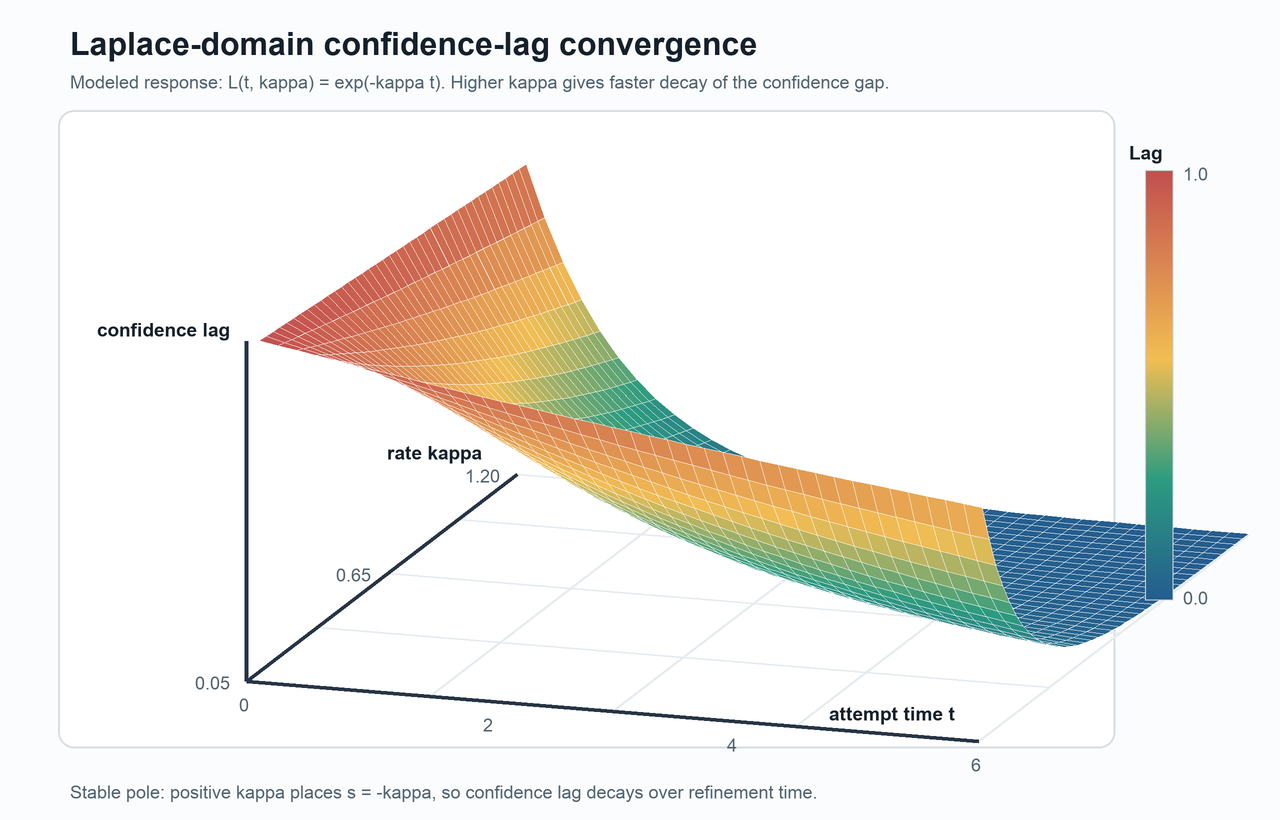
\includegraphics[width=\columnwidth]{generated/laplace_convergence_surface.png}
\caption{Laplace-inspired confidence-lag convergence surface for normalized lag \(\ell(t;\kappa)=e^{-\kappa t}\). Larger \(\kappa\) values yield faster lag decay, consistent with the pole-location condition \(s_L=-\kappa<0\).}
\Description{Three-dimensional surface plot showing confidence lag decreasing over attempt time as convergence rate increases.}
\label{fig:laplace-convergence-surface}
\end{figure}

\clearpage
\subsubsection{Algorithmic Realization}
Algorithms~\ref{alg:e2e-inference} and~\ref{alg:rl-policy-update}
illustrate the described approach in practice.

Algorithm~\ref{alg:e2e-inference} illustrates the full process flow.
It involves obtaining context and generating candidate stories.
It picks a safe prompt arm and improves each story.
A story can be submitted to Jira only after passing the validation, policy, and human review steps.

Algorithm~\ref{alg:rl-policy-update} illustrates the prompt-policy update process.
It calculates a signed reward based on the change in confidence level, reviewer decision, and write back flag.
The reward is mapped to success credit and updated in the selected arm's Beta posterior distribution.

\begin{algorithm}[H]
\DontPrintSemicolon
\footnotesize
\caption{End-to-End RL-Governed Epic-to-Story Inference Pipeline}
\label{alg:e2e-inference}
\KwIn{Epic $E$, connectors $\mathcal{X}$ (Jira/Confluence/Bitbucket), policy state $\mathcal{P}$, thresholds $(\tau_c,\tau_e)$, max attempts $T$}
\KwOut{Created story set $S_{\mathrm{create}}$, audit trace $\mathcal{T}_{\mathrm{audit}}$}
\tcp{Retrieve available context, scale the threshold, and initialize the trace.}
$\tau_{10}\leftarrow 10\tau_c$; $\mathcal{C} \leftarrow$ RetrieveContext$(E,\mathcal{X})$; $\mathcal{T}_{\mathrm{audit}}\leftarrow\emptyset$\;
$S_{\mathrm{cand}} \leftarrow$ GenerateCandidates$(E,\mathcal{C})$\;
\tcp{For each candidate, select a governance-safe arm, enrich, rescore, and validate.}
\ForEach{$s \in S_{\mathrm{cand}}$}{
  $t \leftarrow 1$; $\ell_0 \leftarrow \tau_{10}$; $A_s \leftarrow 0$\;
  \While{$t \le T$}{
    $k_t \leftarrow$ SelectPromptArm$(\mathcal{P}, s, \mathcal{C})$\;
    $s \leftarrow$ EnrichWithPrompt$(s,k_t,\mathcal{C})$\;
    $(R_s,C_s) \leftarrow$ ScoreReadinessConfidence$(s,\mathcal{C})$\;
    $C_{10,t}\leftarrow 10C_s$; $\ell_t \leftarrow \max(0,\tau_{10}-C_{10,t})$\;
    $\widehat{\kappa}_t \leftarrow$ EstimateLaplaceRate$(\ell_{t-1},\ell_t)$\; \tcp*[r]{Diagnostic only}
    $V_s \leftarrow$ ConsistencyValidate$(s)$\;
    LogAttempt$(\mathcal{T}_{\mathrm{audit}},E,s,t,k_t,R_s,C_s,\ell_t,\widehat{\kappa}_t,V_s)$\;
    \If{$(C_s \ge \tau_c)$ \textbf{and} $(V_s=1)$}{\textbf{break}}
    $t \leftarrow t + 1$\;
  }
  \tcp{Determine escalation; policy and explicit human approval remain separate gates.}
  $I_{\mathrm{esc}}(s) \leftarrow \mathbb{1}[C_s < \tau_e] \lor I_{\mathrm{ctx}}(s)$\;
  $(g_{\Pi}(s),A_s) \leftarrow$ PolicyAndHumanGate$(s,I_{\mathrm{esc}}(s))$\;
  $I_{\mathrm{create}}(s) \leftarrow \mathbb{1}[C_s \ge \tau_c \land A_s=1 \land V_s=1 \land g_{\Pi}(s)=1 \land s\in\mathcal{F}_{\mathrm{dup}}]$\;
  \If{$I_{\mathrm{create}}(s)=1$}{
    \If{HashCheckAndIdempotencyPass$(s)$}{ \tcp*[r]{Source and duplicate safety}
      Writeback$(s)$; AddToCreateSet$(S_{\mathrm{create}},s)$\;
    }
  }
}
\Return{$(S_{\mathrm{create}},\mathcal{T}_{\mathrm{audit}})$}\;
\end{algorithm}

\begin{algorithm}[H]
\DontPrintSemicolon
\footnotesize
\caption{RL Prompt Policy Update (Bandit + Governance-Aware Reward)}
\label{alg:rl-policy-update}
\KwIn{Selected-arm state $(\alpha_{k_t},\beta_{k_t},n_{k_t},\bar r_{k_t})$ and recorded outcome $(C^{\mathrm{before}}_{10,t},C^{\mathrm{after}}_{10,t},d_t,w_t)$}
\KwOut{Updated selected-arm state $(\alpha_{k_t},\beta_{k_t},n_{k_t},\bar r_{k_t})$}
\tcp{Build the signed reward from confidence, reviewer decision, and writeback status.}
$r_t \leftarrow (C^{\mathrm{after}}_{10,t}-C^{\mathrm{before}}_{10,t})/10$\;
$r_t \leftarrow r_t+0.2\mathbb{1}[d_t=\texttt{approve}]-0.2\mathbb{1}[d_t\in\{\texttt{reject},\texttt{regenerate}\}]$\;
$r_t \leftarrow r_t+0.1\mathbb{1}[w_t=\texttt{written}]-0.1\mathbb{1}[w_t=\texttt{conflict}]$\;
\tcp{Bound the reward, update the selected arm, and retain audit statistics.}
$r_t \leftarrow \operatorname{clip}(r_t,-1,1)$\;
$q_t \leftarrow (r_t+1)/2$\;
$(\alpha_{k_t},\beta_{k_t}) \leftarrow (\alpha_{k_t}+q_t,\beta_{k_t}+1-q_t)$\;
$n_{k_t} \leftarrow n_{k_t}+1$\;
$\bar r_{k_t} \leftarrow \bar r_{k_t}+(r_t-\bar r_{k_t})/n_{k_t}$\;
\Return{$(\alpha_{k_t},\beta_{k_t},n_{k_t},\bar r_{k_t})$}\;
\end{algorithm}

\FloatBarrier
\subsection{Epic-to-Story Decomposition Method}


\subsubsection{Candidate Generation}
By leveraging epic context and previous stories, the system can produce any required capability archetypes:
\begin{itemize}
  \item UI/interaction story,
  \item API/contract story,
  \item persistence/writeback story,
  \item validation/regression story.
\end{itemize}

This system rejects the archetypes that are already covered in existing summaries via lexical and semantic matching.

This helps avoid the common error of ``story inflation,'' where assistants create tickets that differ in wording but cover the same work.

In the current implementation, the system recognizes any embedded epic description as a first-class piece of evidence. When an epic is filled with design signals such as solution-design headings, scaling, formulas, APIs and workflows, validation, roll-back considerations, and testing considerations, the system will output a \texttt{jira\_embedded\_context} piece of evidence. This makes the decomposition resilient to the common enterprise challenge where Confluence links are unavailable at the time of execution, while the epic still contains enough design information for bounded planning. In case when the epic has only links and those links are not available, the system avoids the generation of any placeholders and returns the context unavailability message.

\subsubsection{Story Point Assignment}
Initial estimates are derived from complexity priors:
\begin{equation}
\mathrm{SP}(s) = f(\xi_{\text{scope}}, \xi_{\text{integration}}, \xi_{\text{risk}}, \xi_{\text{unknown}}),
\end{equation}
with the four $\xi$ factors representing normalized priors for the complexity of scope, integration, risk, and uncertainty. The resulting measure is categorized using Fibonacci-like buckets of 3, 5, and 8. In the current implementation, the default values are deterministic (3/5) and may be learned in future implementations.

Deterministic baseline is an intended choice. It guarantees consistent behavior in initial phases of use and avoids estimation variability until there is enough history to learn from. It also represents a conservative approach to evaluation whereby the value brought in by automation is compared with deterministic baseline performance before applying any other estimation techniques.

\subsubsection{Iterative Enrichment}
For each candidate story $s$:
\begin{enumerate}
  \item run semantic analysis,
  \item calculate readiness/confidence,
  \item if $C(s)<\tau_c$, provide guidance and repeat the enrichment process within a bounded attempt budget,
  \item provide a structured story payload.
\end{enumerate}

Enrichment increases as each iteration brings explicit feedback from reviewers, such as missed edge cases, unresolved dependencies, or ambiguous non-functional requirements. Thus, the refinement process becomes a collaboration, not just prompting. The distinction is important for successful interaction between human and AI \cite{R56,R57}.

Moreover, in one embodiment, the output of the enrichment process follows a canonical, strongly typed schema:\linebreak
\texttt{problem\_statement}, \texttt{actor\_value}, \texttt{functional\_scope}, \texttt{nfr\_constraints}, \texttt{acceptance\_criteria},\linebreak
\texttt{dependency\_map}, \texttt{risk\_register}, and \texttt{test\_considerations}. The high degree of typing ensures interoperability of the result with tools for reviews, analytics, and policies and removes ambiguity caused by the informal nature of the free-form text.

An analysis of coverage on the epic level can be done through the capability matrix. Its rows correspond to the capability dimensions such as UI, API, data, observability, resiliency, and security, while its columns represent the suggested stories. The system is able to detect undercovered dimensions and generate candidate stories accordingly. It alters the decomposition process from merely generative to constrained generation with clear objectives.

\subsubsection{Ablation Execution Algorithm}
Algorithm~\ref{alg:ablation-exec} presents the way how all four modes are implemented for the same epic unit. For each mode, the algorithm activates only the components which fall under this condition, uses the same scorecard, and provides measurements of quality, efficiency, governance, performance, and assessment time.

\begin{algorithm}[H]
\DontPrintSemicolon
\footnotesize
\caption{Ablation-Mode Execution for B0/B1/B2/B3 Comparison}
\label{alg:ablation-exec}
\KwIn{Epic unit $E_u$, mode $m \in \{\mathrm{B0},\mathrm{B1},\mathrm{B2},\mathrm{B3}\}$}
\KwOut{Metric row $(Q_m,\mathrm{Eff}_m,G_m,\mathrm{Composite}_m,\mathrm{Time}_m)$}
\tcp{Mode schema only; not every evidence block executes every condition.}
\eIf{$m=\mathrm{B0}$}{
  ExecuteManualReferenceCore$(E_u)$\; \tcp*[r]{Independent manual package required}
}{
  ExecuteTemplateCore$(E_u)$ if $m=\mathrm{B1}$\;
  ExecuteGenericLLMCore$(E_u)$ if $m=\mathrm{B2}$\;
  ExecuteFullJiraEnhancerCore$(E_u)$ if $m=\mathrm{B3}$\;
}
\tcp{Disable B3-only components in baseline modes.}
\If{$m\neq\mathrm{B3}$}{
  Disable components excluded from mode $m$ (critic loop / context packer / validator / governed writeback)\;
}
\tcp{Use one scorer; each row retains its measured or analytical status.}
Collect metrics using the same scorer and schema across all modes\;
Compute $Q_m$ (quality), $\mathrm{Eff}_m$ (efficiency), $G_m$ (governance), $\mathrm{Composite}_m$, and $\mathrm{Time}_m$\;
\Return{$(Q_m,\mathrm{Eff}_m,G_m,\mathrm{Composite}_m,\mathrm{Time}_m)$}\;
\end{algorithm}

\subsection{Policy and Governance Layer}

The policy and governance layer controls whether a candidate story may move towards Jira creation. It checks confidence, available context, policy rules, validation, and human approval. The AI may generate and refine a story, but it cannot approve the final writeback.
First, the system checks whether a story needs additional human review:
\begin{equation}
I_{\mathrm{esc}}(s)
= \mathbb{1}[C(s) < \tau_e] \lor I_{\mathrm{ctx}}(s).
\end{equation}
where $\tau_e$ is the normalized escalation threshold and $I_{\text{ctx}}(s)$ denotes a partial external-context condition. This predicate cannot substitute the explicit approval indicator $A(s)$. Here, $I_{\mathrm{esc}}(s)\in\{0,1\}$ is the escalation indicator for candidate story $s$. It equals 1 when the confidence is below $\tau_e$ or when external context is incomplete. In this case, the story requires additional human review. Otherwise, it equals 0. Escalation does not replace the mandatory human-approval gate.

The system next checks whether candidate story $s$ is eligible for creation:
\begin{equation}
\begin{aligned}
g_{\Pi}(s) ={}& \mathbb{1}[\Pi(s)=\textsc{allow}],\\
I_{\mathrm{create}}(s) ={}&
\mathbb{1}[C(s)\ge\tau_c \land A(s)=1 \land V(s)=1 \land g_{\Pi}(s)=1 \land s\in\mathcal{F}_{\mathrm{dup}}],
\end{aligned}
\end{equation}
Here, $\mathbb{1}[\cdot]$ is an indicator function. It returns 1 when a condition is true and 0 otherwise. The term $\Pi(s)$ is the decision made by the active policy. Therefore, $g_{\Pi}(s)=1$ means that the policy allows the story.

The creation rule contains five gates. First, $C(s)$ must reach the confidence threshold $\tau_c$. Second, $A(s)=1$ confirms human approval. Third, $V(s)=1$ confirms that validation has passed. Fourth, $g_{\Pi}(s)=1$ confirms policy permission. Finally, $s\in\mathcal{F}_{\mathrm{dup}}$ confirms that the story is not a duplicate.

The value $I_{\mathrm{create}}(s)=1$ only when all five gates pass. If any gate fails, the story is not eligible for creation. This value indicates eligibility only. It does not mean that Jira has already been updated. The source-hash and idempotency checks must also pass, as shown in Algorithm~\ref{alg:e2e-inference}. The conflict and target checks are applied by the writeback model described below.

Confidence and human approval are important gates. However, neither gate is sufficient by itself. Validation, policy permission, and duplicate control are also required. This design keeps the final decision with a reviewer and supports appropriate reliance on automation \cite{R56,R75}.

Approval is always attached to a concrete execution run. This way, it can be evaluated in terms of the policy used during the actual execution of the decision, regardless of modifications made to the thresholds afterward. Traceability is important for regulated environments, in which the reproduction of the process is even more important than the outcome itself.

The governance level may also set the approval rules based on the role of the reviewer: changes to the API contract are approved by the domain owner, whereas changes to authentication flow require security approval. Such approval-routing criteria can be represented as policy predicates based on generated metadata and evidence tags.

\subsection{Conflict-Safe Writeback Model}

The previous section decides whether a candidate may enter the creation stage. It does not make the final change in Jira. In this section, \emph{writeback} means that final Jira change. Approval and writeback may happen at different times. During this gap, the source issue, draft, policy, or target may change. A request may also be retried. The model below blocks stale changes and prevents duplicate creation.

We use two protection levels in this section. A2 combines a source-hash check with atomic idempotency. A3 adds a source-bound transaction envelope. These arrangements are evaluated later in Table~\ref{tab:mutation-safety-ablation}.

\paragraph{Approval-bound context.}
An approval flag records the reviewer's decision. However, it does not record the exact context that was approved. A3 therefore stores this context in an approved transaction envelope, denoted by $\mathcal{E}_a$:
\begin{equation}
\mathcal{E}_a=(r_{\mathrm{run}},i_{\mathrm{issue}},h_s,\nu_s,\nu_d,h_d,\nu_{\Pi},h_{\Pi},\mathcal{T}_{\mathrm{target}},a_{\mathrm{dec}},u_{\mathrm{rev}},t_a),
\end{equation}
where $r_{\mathrm{run}}$ identifies the run and $i_{\mathrm{issue}}$ identifies the issue. The pair $(h_s,\nu_s)$ records the approved source hash and revision. The pair $(\nu_d,h_d)$ records the approved draft version and payload hash. The pair $(\nu_{\Pi},h_{\Pi})$ records the policy version and snapshot hash. The set $\mathcal{T}_{\mathrm{target}}$ lists the allowed Jira targets. Finally, $a_{\mathrm{dec}}$, $u_{\mathrm{rev}}$, and $t_a$ record the approval result, reviewer, and time.

The system hashes the complete envelope to obtain the transaction identifier $I_{\mathrm{tx}}=H(\mathcal{E}_a)$. The A3 idempotency key then binds this transaction to the issue:
\begin{equation}
K_{A3}=H(I_{\mathrm{tx}},i_{\mathrm{issue}}).
\end{equation}

\paragraph{Runtime validation.}
Immediately before writeback, the validator builds the runtime envelope $\mathcal{E}_t$. It has the same fields as $\mathcal{E}_a$. The validator rereads the current source, draft, policy, and target values. It carries forward the run, issue, and approval metadata from the approved envelope.

The system permits a mutation only when the two envelopes match and the decision is still \textsc{approve}:
\begin{equation}
\operatorname{permit}(\mathcal{E}_a,\mathcal{E}_t)
=\mathbb{1}[\mathcal{E}_a=\mathcal{E}_t \land a_{\mathrm{dec}}=\textsc{approve}].
\end{equation}
An ABA change occurs when the source moves from state A to B and later returns to the same visible content A. Its revision has still changed. The envelope comparison detects this case. It also detects draft regeneration, policy drift, and target drift. A matching Jira text hash alone is therefore not sufficient.

\paragraph{Source-conflict check.}
The system also calculates a hash of the current normalized issue state:
\begin{equation}
h_{\text{current}} = H(\text{normalized issue state}),
\end{equation}
It compares this value with the approved source hash $h_{\mathrm{expected}}:=h_s$. A mismatch moves the item to the conflict path, and Jira is not changed. Here, $\operatorname{write}(s)=1$ means that story $s$ is written to Jira. Within the declared validator and fault model, the write authorization rule is:
\begin{equation}
\Pr(\text{write}(s)=1 \mid h_{\text{current}}\ne h_{\text{expected}})=0.
\end{equation}

\paragraph{Retry protection.}
While the source check protects from a stale write, repeated requests might cause duplicates. A2 addresses this issue by introducing a payload-level idempotency key:
\begin{equation}
K_{A2} = H(\text{normalized payload},\;\text{target epic},\;\text{policy version}).
\end{equation}
Requests with the same normalized payload, target epic, and policy version will have the same A2 key. A3 employs the envelope-level key mentioned above. Since $I_{\mathrm{tx}}=H(\mathcal{E}_a)$, its key is equivalently $H(H(\mathcal{E}_a),i_{\mathrm{issue}})$. This binds the retry to the approved context.

The key is verified and reserved atomically before mutation. The hashing alone is not enough since deterministic field ordering makes sure that two logically equivalent payloads have the same hash input. Thus, the request may be treated as the same operation and not a new one. In case the approved state was changed, the story should be revalidated and reapproved. All guarantees hold for the implementation and fault model discussed in Table~\ref{tab:mutation-safety-ablation}.

\paragraph{Per-story and batch outcomes.}
The previous rules decide whether one story may be written. A run may have several candidate stories, so the system logs each outcome individually. Let $o_s$ denote the outcome of candidate $s$, where
\[
o_s\in\{\textsc{created},\textsc{already\_exists},\textsc{not\_approved},\textsc{create\_failed}\}.
\]
For a candidate batch $\mathcal{B}_{\mathrm{batch}}$, the overall status follows this precedence rule:
\begin{equation}
\operatorname{status}(\mathcal{B}_{\mathrm{batch}})=
\begin{cases}
\textsc{created}, & \exists s\in \mathcal{B}_{\mathrm{batch}}: o_s=\textsc{created},\\
\textsc{failed}, & \exists s\in \mathcal{B}_{\mathrm{batch}}: o_s=\textsc{create\_failed},\\
\textsc{already\_exists}, & \exists s\in \mathcal{B}_{\mathrm{batch}}: o_s=\textsc{already\_exists},\\
\textsc{failed}, & \text{otherwise}.
\end{cases}
\end{equation}
The rules are processed from top to bottom. A success in the creation has priority. If nothing has been created, the creation error leads to \textsc{failed}. If neither of these conditions is true, the duplicate leads to \textsc{already\_exists}. A batch with only unapproved stories leads to \textsc{failed}. The detailed per-story results remain available in every case. The reviewer can therefore see each skipped item, its reason, any connector error, and the existing Jira key for a duplicate.

\subsection{API and UI Innovation}

\subsubsection{Workflow API}
The API supports two connected tasks. The first task enriches existing Jira items through a human review and revision loop. The second task decomposes an epic into candidate stories. Jira mutation remains separate from both tasks.

\paragraph{Run creation and inspection.}
\texttt{POST /api/v1/runs} starts an enrichment run for an issue, sprint, epic, or release. \texttt{GET /api/v1/runs/\allowbreak\{runId\}} returns the overall run status. \texttt{GET /api/v1/runs/\allowbreak\{runId\}/\allowbreak{}items/\allowbreak\{issueKey\}} returns the current draft. It also returns the evidence, warnings, readiness, confidence, policy state, and prompt-selection details. These read endpoints allow a reviewer to inspect the result before making a decision.

\paragraph{Human guidance and revision.}
The reviewer does not need to accept the first draft. \texttt{POST /api/v1/runs/\allowbreak\{runId\}/\allowbreak{}items/\allowbreak\{issueKey\}/\allowbreak{}approval} records a decision for one item. The allowed values are \texttt{approve}, \texttt{reject}, \texttt{regenerate}, \texttt{user\_input}, and \texttt{prompt}. The \texttt{user\_input} decision carries a human suggestion. The \texttt{prompt} decision carries a reviewer-written instruction for further modification. Both forms of guidance are sent back to the reasoning process, which produces a revised draft.

The run-level endpoint, \texttt{POST /api/v1/runs/\allowbreak\{runId\}/\allowbreak{}approval}, applies the same decision and guidance to every item in the run. The system may also ask a clarification question. In this case, \texttt{POST /api/v1/runs/\allowbreak\{runId\}/\allowbreak{}items/\allowbreak\{issueKey\}/\allowbreak{}interaction-answer} records the human answer and continues the revision. Human suggestions and follow-up prompts are therefore part of the API workflow.

\paragraph{Controlled writeback.}
\texttt{POST /api/v1/runs/\allowbreak\{runId\}/\allowbreak{}items/\allowbreak\{issueKey\}/\allowbreak{}writeback} writes one approved item after the policy, validation, source-conflict, and retry checks. \texttt{POST /api/v1/runs/\allowbreak\{runId\}/\allowbreak{}writeback} applies this operation across the run. Each item still receives its own result. This preserves item-level reasons for a successful, blocked, conflicting, or repeated request.

\paragraph{Epic story decomposition.}
\texttt{POST /api/v1/epics/\allowbreak\{epicKey\}/\allowbreak{}stories/\allowbreak{}suggest} reads the epic, existing child stories, and available evidence. It returns editable story candidates with readiness, confidence, threshold status, warnings, and evidence references. It does not create Jira stories.

\texttt{POST /api/v1/epics/\allowbreak\{epicKey\}/\allowbreak{}stories/\allowbreak{}create} receives the reviewed story payloads. It checks confidence and approval. It skips matching existing summaries and attempts to create only the remaining stories. Its response lists created and skipped items, including duplicate and creation-failure reasons.

The API therefore supports a full cycle: inspect, suggest, provide human guidance, revise, approve, and write back. Human users and controlled clients use the same contracts and governance checks.

\subsubsection{Console Workflow}
The console exposes the same workflow in three connected views. The enrichment view starts a run. It shows each Jira draft with its evidence, warnings, readiness, confidence, and selected prompt. The review view allows the user to approve, reject, request regeneration, provide a human suggestion, or submit a Jira-specific prompt for further modification. The same guidance can be applied to one Jira or to all Jira items in the run.

\begin{samepage}
The \textbf{Epic Story Breakdown} view provides the following features:
\begin{enumerate}
  \item epic-key and project-key inputs,
  \item the suggestion action, which reads the epic and proposes child stories,
  \item an editable structured payload for reviewing each story, with an \texttt{approved} flag per story,
  \item the approved-story creation action for writing back qualified rows.
\end{enumerate}
\end{samepage}

The reviewer can edit the generated content, add missing context, or provide a new prompt before approval. Writeback remains a separate action. This prevents a revision request from being treated as permission to change Jira.

Human-led and agent-led operations are both provided via the API. The human reviewer assesses the narrative and the possible risks through the console, whereas controlled agents or pipelines do that using the same endpoints according to deterministic payload contracts. This allows governed integration with release-planning bots, PM dashboards, and governance data lakes.

The UI focuses on ``decision visibility,'' giving the reviewer the sources of confidence, warnings, policy reason codes, approval provenance, reasons for skipping duplicates, and preserved retry selections for each story candidate. This discourages reviewers from treating confidence as an unsupported number and enables quicker and better accept, reject, or retry decisions. The design seeks appropriate trust rather than maximum automation, reflecting evidence that human--AI team performance depends on users' mental models of system behavior \cite{R56,R57,R76}.

\FloatBarrier
\section{Evaluation Design and Evidence}

Evaluation of evidence is classified by the way evidence is acquired and the claims it supports. This ensures that field observations, controlled fault injections, and generated sensitivity analyses are not treated as equivalent empirical samples. Table~4 specifies the units of analysis and inference limits for each evidence block.

\begin{table*}[t]
\centering
\footnotesize
\caption{Evidence hierarchy and claim boundaries. ``Generated'' denotes deterministic formula-based perturbation or scoring, not an observed execution of the named baseline.}
\label{tab:evidence-hierarchy}
\begin{tabularx}{\textwidth}{@{}p{0.19\textwidth}p{0.18\textwidth}p{0.22\textwidth}X@{}}
\toprule
Evidence block & Unit and scale & Primary use & Explicit inference boundary \\
\midrule
Authenticated Jira field trace & 70 story endpoints; two waves; 14 epics & RQ1 workflow feasibility and RQ2 endpoint telemetry & No randomized control, rejected case, or downstream delivery outcome; independent content ratings are reported separately. \\
Authenticated-output artifact assessment & Two independent reviewers; 69 full-text stories; 14 epic packages; three masked repeats per reviewer & RQ1 artifact quality and RQ2 reviewability & B3-only absolute assessment; no baseline comparison, downstream outcome, or cross-organization generalization. \\
Matched blinded baseline assessment & Five reviewers; 42 primary packages (14 inputs $\times$ B1/B2/B3); 210 stories; four masked repeats per reviewer & RQ4 package quality, readiness, and reviewer-recorded effort & Reviewers 3--5 form the primary analysis; one portfolio, no manual baseline, no downstream outcome, and no empirical method-origin guess. \\
Held-out learned-selection diagnostic & Three preselected packets; B2 and B3; two blinded model evaluators; six paired judgments & Exploratory RQ4 text quality and model-evaluator-suggested follow-up prompts & Descriptive only; refinement passes and output length differ; it does not isolate the selection-policy effect. \\
Controlled mutation-safety ablation & Nine scenarios; 2,000 payloads/scenario; four arrangements; 72,000 method-level observations & RQ3 stale-state, retry, and duplicate handling & Scenario-balanced fault injection; rates are not estimates of production incident prevalence. \\
Internal generated-unit sensitivity analysis & 5,000 formula-derived units per method & Stress-test the declared scoring and composite-index model & B0--B3 metrics are generated; this is not a measured manual-versus-LLM experiment. \\
Public issue-text sensitivity analysis & 300 SWE-bench Lite issue records & Test whether the scoring pipeline accepts public issue text & No patches are generated and no SWE-bench tests are executed; this is not a resolution benchmark result. \\
\bottomrule
\end{tabularx}
\end{table*}

For reproducibility, the evidence units are organized around story-level endpoints, confidence and readiness summaries, policy decisions, and connector outcomes. The fault-injection units use a fixed random seed and the same transaction schedules for each arrangement. In turn, the generated-unit blocks use their corresponding seeds and transformations. In accordance with empirical software-engineering guidelines on clarity of context, measures, and analysis procedures, we provide the reporting details in this format \cite{R54,R71,R55,R70}.

\FloatBarrier
\section{Results and Comparative Analysis}

\subsection{Authenticated Jira Deployment Evidence (RQ1--RQ2)}

Figure~\ref{fig:performance-raincloud-combined} presents the authenticated endpoint summary and generated-unit raincloud side by side while stating their evidence status explicitly. Panel~(a) is based on the 70 live Jira story endpoints observed during two authenticated deployment waves. It reports story-level terminal confidence rather than aggregating the data into the older nine-row issue summary, preserving the paired pre- and post-endpoints used in the descriptive and bootstrap analyses below. Panel~(b) presents the scoring-model distribution for 5,000 formula-generated sensitivity samples anchored to observed Jira Enhancer data.

\begin{figure*}[t]
\centering
\begin{subfigure}[t]{0.485\textwidth}
\centering
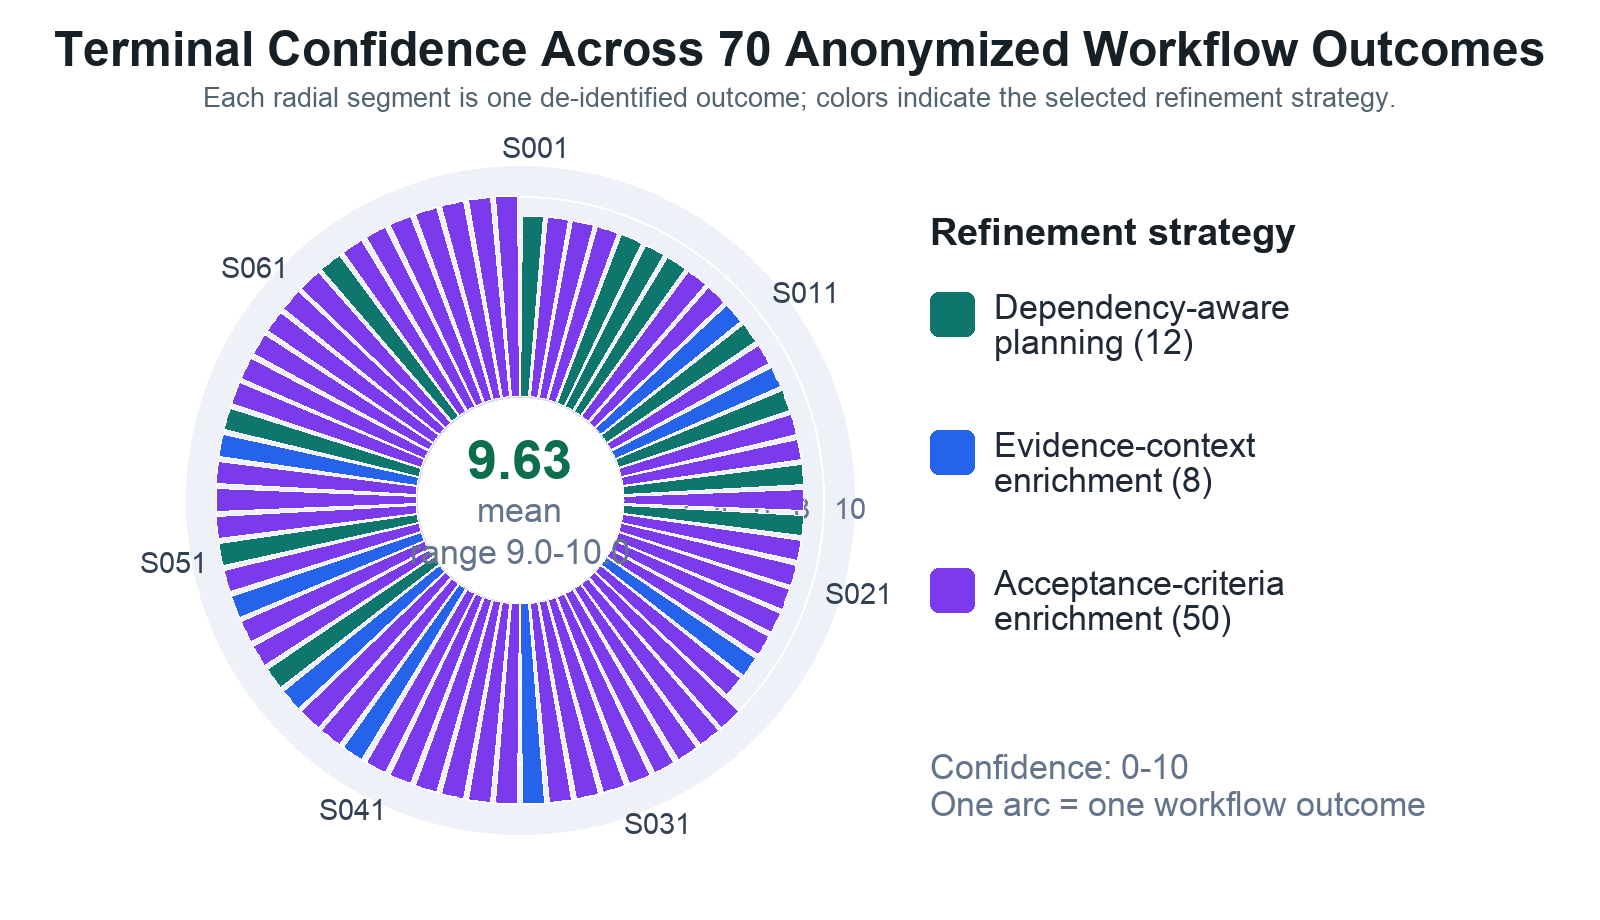
\includegraphics[width=\linewidth,height=0.245\textheight,keepaspectratio]{generated/performance_confidence_readiness.png}
\caption{Authenticated live-story confidence.}
\label{fig:performance-summary}
\end{subfigure}\hfill
\begin{subfigure}[t]{0.485\textwidth}
\centering
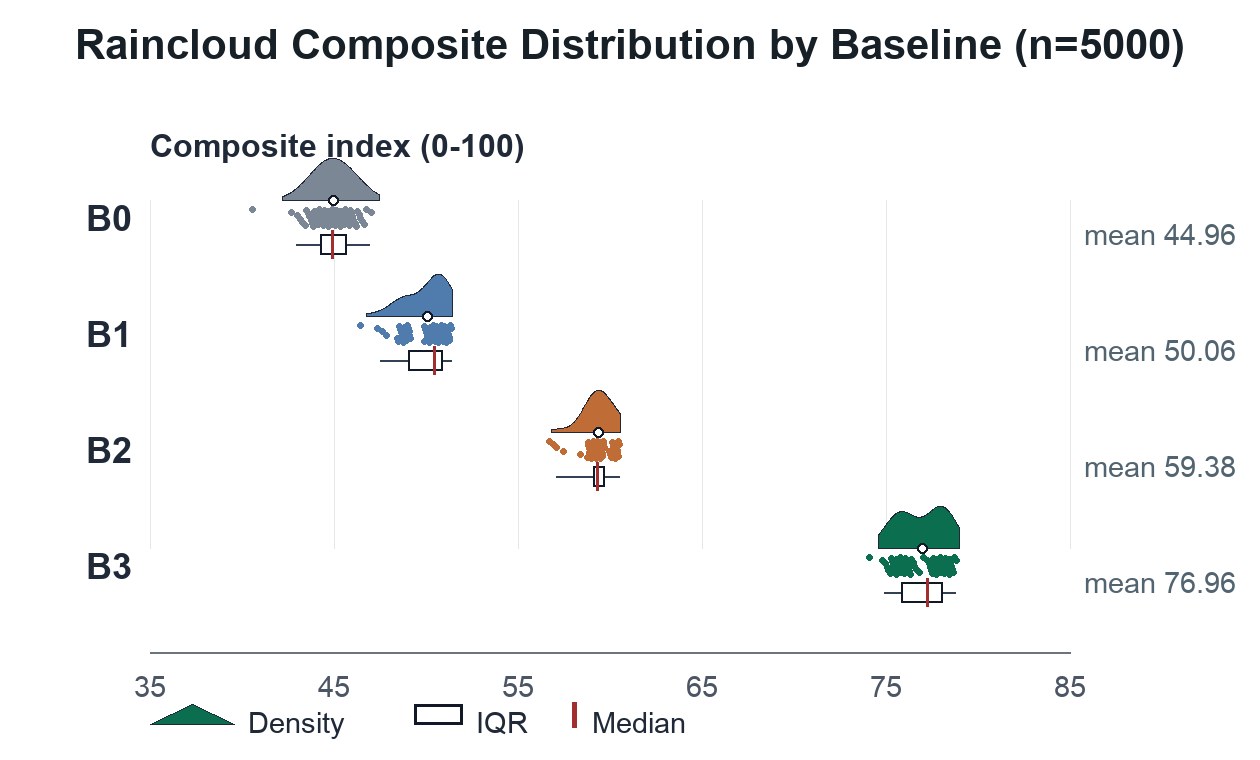
\includegraphics[width=\linewidth,height=0.245\textheight,keepaspectratio]{generated/comparative_5000_boxplot.png}
\caption{Scoring-model composite distributions.}
\label{fig:comparative-5000-raincloud}
\end{subfigure}
\caption{Two performance views with different evidence status. (a) Terminal confidence for all 70 authenticated live Jira story outcomes. Each radial segment represents one story, ordered by terminal confidence and colored by the selected refinement strategy. (b) Raincloud distribution of scoring-model composite indices over 5,000 generated units per method, showing density, sampled values, IQR, median, and mean. Panel (b) compares scoring-model outputs across B0--B3. The values are anchored to observed Jira Enhancer data, while the 5,000 units are formula-generated sensitivity samples.}
\Description{Two side-by-side charts with distinct evidence status. Panel (a) is a radial bar chart of terminal confidence for 70 authenticated live Jira story outcomes. Panel (b) is a raincloud plot of scoring-model composite-index distributions for B0, B1, B2, and B3 over 5,000 generated units per method.}
\label{fig:performance-raincloud-combined}
\end{figure*}

Figure~\ref{fig:performance-raincloud-combined}(a) summarizes the distribution of terminal endpoints. Each arc represents one Jira story, with longer arcs indicating higher displayed confidence $C_{10}$ on the zero-to-ten scale; color identifies the selected refinement strategy. All 70 records reached a governed terminal state at $C_{10}\ge 9$. Because neither deployment wave retained rejected or below-threshold stories, the chart shows successful-path feasibility rather than field-wide acceptance performance. Panel~(b) gives a succinct distributional check of the declared composite-index formulas. The separation among B0--B3 is induced by the scoring model and seeded perturbations, and thus should not be interpreted as measured superiority over executed baselines.

For adaptive-policy telemetry, the current evidence base consists of two authenticated and verified Jira deployment waves: a five-epic wave with 25 terminal story records and a nine-epic Confluence-derived wave with 45 terminal story records. Together, the waves provide a total of 70 persisted endpoint pairs containing confidence, shaped reward, loss, lag, selected prompt strategy, approval, and writeback status. Each current endpoint has one terminal attempt index, while intermediate live refinement attempts were not persisted. Hence, the endpoint data support paired confidence analysis, but do not support an observed multi-step learning-curve claim.

\begin{table*}[t]
\centering
\small
\caption{Accumulated live Jira evidence across two authenticated deployment waves. The table distinguishes the observed production-style outcome signal from the larger comparative simulation and public-benchmark evidence blocks.}
\label{tab:cumulative-live-evidence}
\begin{tabularx}{\textwidth}{@{}p{0.22\textwidth}p{0.27\textwidth}X@{}}
\toprule
Evidence dimension & Observed value & Interpretation \\
\midrule
Cumulative scope over lifetime & 2 authenticated and validated waves, 70 story outcomes & Consists of one previous five-epic deployment wave (25 outcomes) and one subsequent nine-epic Confluence-derived AES deployment wave (45 outcomes). \\
Governing terminal conditions & 70/70 (100.0\%); 69 created, 1 duplicate-safe existing record & All candidates reached a governed terminal state, and the existing record was validated without creating a duplicate. \\
Reward distribution & range 0.40--0.70; mean 0.5171; cumulative 36.20 & The reward is not a static indicator of success; it depends on confidence lift and whether writeback occurred. \\
Loss from terminal confidence gap & mean 0.00 & The normalized difference from target confidence was 0 for all persisted outcomes; it is not an estimate of sequential training loss. \\
Refinement strategy distribution & Dependency-aware planning: 12, Evidence-context enrichment: 8, Acceptance-criteria enrichment: 50 & The evidence covers several policy-governed refinement strategies rather than one hard-coded prompt path. \\
\bottomrule
\end{tabularx}

\end{table*}

The latest validated wave is shown separately because it traversed the complete Confluence-to-Jira path involving nine additional epics. Table~6 gives the statistics for this wave: Jira Enhancer produced or verified 45 story records, created 44 new stories, detected one pre-existing story through duplicate-safe link checking, and associated all 45 story records with the intended parent epic. All 44 newly created payloads contained the four audited elements: an external evidence reference, acceptance criteria, test criteria, and operational-observability criteria. The pre-existing story is excluded from the payload denominator because its generated payload was unavailable for the same audit.

\begin{table*}[t]
\centering
\small
\caption{Most recent authenticated live batch derived from Confluence. The table reports the 45-story expansion that followed the earlier 25-story run and forms part of the cumulative 70-outcome evidence base.}
\label{tab:latest-live-batch}
\begin{tabularx}{\textwidth}{@{}p{0.22\textwidth}p{0.26\textwidth}X@{}}
\toprule
Evidence dimension & Observed value & Interpretation \\
\midrule
Deployment scope & 9 epics, 45 stories & Exercises the full Confluence-to-Jira planning path at batch level. \\
Writeback outcome & 44 created; 1 duplicate-safe link check & Distinguishes new issue creation from reuse of an existing story. \\
Parent-epic binding & 45/45 (100.0\%) & Confirms that every generated or checked story is attached to its intended epic. \\
Generated-payload coverage & 44/44 new stories (100.0\%) & All newly created payloads include the evidence reference, acceptance criteria, tests, and operational criteria; the pre-existing linked record is excluded. \\
RL outcome telemetry & 45 outcomes; reward 0.50--0.70; mean 0.5822 & Rewards vary with confidence lift instead of treating all accepted stories as a flat success. \\
Refinement-strategy signal & Dependency-aware planning: 4, Evidence-context enrichment: 5, Acceptance-criteria enrichment: 36 & Shows which policy-selected refinement strategies were used in the live batch. \\
Convergence signal & mean terminal loss 0.00 & The confidence-gap objective reached zero for the recorded live outcomes. \\
\bottomrule
\end{tabularx}

\end{table*}

\begin{table*}[t]
\centering
\small
\caption{Observed live endpoint and connector statistics. Confidence intervals quantify sampling uncertainty within the recorded story set; they do not remove portfolio selection or within-epic dependence.}
\label{tab:live-endpoint-statistics}
\begin{tabularx}{\textwidth}{@{}p{0.24\textwidth}p{0.18\textwidth}p{0.22\textwidth}X@{}}
\toprule
Observed measure & Estimate & 95\% interval & Inference boundary \\
\midrule
Paired confidence change & +2.17 points ($n=70$) & [1.94, 2.40] bootstrap CI & System telemetry; not an independent human rating of story quality. \\
Positive confidence change & 70/70 (100.0\%) & [94.8\%, 100.0\%] Wilson CI & Paired endpoint diagnostic; all rows were retained and no zero deltas occurred. \\
New Jira issue creation & 69/69 (100.0\%) & [94.7\%, 100.0\%] Wilson CI & Conditional on approved, non-duplicate candidates in the two recorded waves. \\
Latest-wave parent binding & 45/45 (100.0\%) & [92.1\%, 100.0\%] Wilson CI & Direct connector outcome for nine epics; no cross-project generalization is implied. \\
Generated-payload criteria coverage & 44/44 (100.0\%) & [92.0\%, 100.0\%] Wilson CI & The pre-existing duplicate-safe record is excluded because its generated payload was unavailable. \\
\bottomrule
\end{tabularx}

\end{table*}

Table~\ref{tab:live-endpoint-statistics} gives the story-level uncertainty based on 50,000 fixed-seed bootstrap resamples \cite{R97}; binary connector outcomes are evaluated with Wilson intervals. Mean confidence increased from 7.46 (SD 0.56) to 9.63 (SD 0.49), a paired mean increase of 2.17 points (95\% bootstrap CI [1.94, 2.40]), while the median difference was 2.50 (IQR 1.00--3.00). All 70 changes were positive (exact two-sided sign test, \(p=1.69\times10^{-21}\)). This shows consistent movement of the system-derived score toward its configured threshold. The blinded review offers a separate assessment of content quality, but confidence remains a system-derived metric rather than a calibrated probability of successful deployment.

\subsection{Blinded Independent Artifact Assessment (RQ1--RQ2)}

\noindent\textit{RQ1: How can a human-AI workflow split underspecified software epics into reviewable implementation stories without compromising human authority over acceptance and writeback?}\par
\noindent\textit{RQ2: How can machine confidence, evidence provenance, and policy gates be combined to help reviewers determine whether AI-generated planning records are reliable enough for action?}\par

Two software-engineering reviewers independently assessed anonymized planning artifacts from the authenticated waves. The review materials omitted method labels, Jira and epic identifiers, internal links, author fields, confidence, readiness, reward, loss, policy-arm values, timestamps, and writeback status. Artifact order was randomized independently for each reviewer. All 70 outcomes remained in scope: 69 stories with full payloads received numerical ratings, while the one pre-existing summary-only record was retained for accounting and marked not rateable. Each reviewer also assessed all 14 five-story epic packages. Three masked repeats per reviewer were excluded from the primary estimates and retained only for descriptive intra-rater checks.

The prespecified story rubric used six dimensions on a 1--5 anchored scale: scope fit, clarity, acceptance/testability, dependency/risk treatment, granularity/actionability, and implementation readiness. The package rubric used coverage breadth, non-redundancy, decomposition coherence, dependency sequencing, and overall readiness. Reviewer scores were first averaged within each artifact. The primary story interval used 50,000 bootstrap resamples of complete epic clusters, preserving the dependence among stories from the same epic.

\begin{table}[H]
\centering
\footnotesize
\caption{Independent blinded ratings on the prespecified 1--5 scale (69 full-text stories and 14 epic packages).}
\label{tab:blinded-artifact-review}
\begin{tabularx}{\columnwidth}{@{}Xr@{}}
\toprule
Measure & Mean \\
\midrule
Story composite & 3.98 \\
Scope fit & 4.97 \\
Clarity & 3.90 \\
Acceptance and testability & 3.62 \\
Dependency and risk treatment & 3.62 \\
Granularity and actionability & 4.26 \\
Implementation readiness & 3.54 \\
\midrule
Epic-package composite & 4.41 \\
Coverage breadth & 4.86 \\
Non-redundancy & 4.79 \\
Decomposition coherence & 4.75 \\
Dependency sequencing & 4.04 \\
Overall package readiness & 3.64 \\
\bottomrule
\end{tabularx}
\end{table}

The mean story composite was 3.98/5 (epic-clustered 95\% bootstrap CI [3.85, 4.11]). When story composites were aggregated within each epic, all 14 epic means exceeded the neutral midpoint of 3 (two-sided Wilcoxon signed-rank test \cite{R99}, \(p=0.00098\)). The package composite mean was 4.41/5, and all 14 package composites also exceeded 3 (\(p=0.00087\)). Neither reviewer recorded an unsupported claim in a rateable story. The numerical profile is more informative than a single readiness label: scope fit and epic-level coverage were high, whereas acceptance/testability, dependency/risk treatment, and implementation readiness retained more room for reviewer-guided refinement.

Absolute-agreement ICC(2,1) was 0.45 for the story composite and 0.58 for the package composite. Exact agreement across story dimensions ranged from 30.4\% to 94.2\%, while agreement within one scale point ranged from 91.3\% to 100\%; every package dimension was within one point in all cases. Some weighted kappa values were near zero despite high observed agreement because variability was low near the top of the scale. We therefore report exact agreement, agreement within one point, and ICC together with kappa rather than relying on kappa alone. Both reviewers reproduced the same composite score for all three masked repeats, although three repeated pairs per reviewer provide only a limited check of consistency.

The reviewers used different cutoffs for categorical decisions. Reviewer~1 labeled 61 stories ``Minor revision'' and 8 ``Major revision'' stories, whereas Reviewer~2 labeled 14 stories ``Ready,'' 48 ``Minor revision,'' and 7 ``Major revision.'' We thus do not aggregate these categories into an overall acceptance rate or state unanimity of readiness. An appropriate interpretation is that the system produced consistent, well-decomposed packages and high-quality artifacts in general, and human review was beneficial for criteria clarification, dependencies, risks, and execution particulars. This block examined only Jira Enhancer outputs; thus, it did not compare the system against manual, template-based, or generic-LLM baselines.

\subsection{Matched Blinded Baseline Comparison (RQ4)}

\noindent\textit{RQ4: How does a governed human-AI workflow perform, relative to executable template/rule and generic-LLM baselines, on decomposition quality, review effort, and implementation readiness?}\par

For the matched experiment, we held frozen the same 14 de-identified epic and evidence packages for the three methods. Each method produced five stories per package, according to a common schema. B1 ran the deterministic evidence-section parser and candidate builder. When the parser returned fewer than five stories, a declared static completion rule filled the remaining slots; this occurred for 24 of the 70 B1 stories. B2 and B3 passed through the authenticated OpenAI Codex service using model \texttt{gpt-5.6-sol} at ultra reasoning effort and the same evidence limitation. B2 made one generic generation request per epic, without a critic pass, confidence feedback, policy gate, retries, or reviewer fixes. B3 initially planned the epic and subsequently used Jira Enhancer's story-level enrichment with the bounded critic loop, scoring, and policy validation. Human approval and Jira writeback were off for each method.

Resource consumption is part of the treatment definition. B1 made zero model requests. B2 made 14 successful requests, one for each package, while B3 made 173: 14 planning requests and 159 story-enrichment attempts. The total execution times were 2,087 seconds for B2 and 19,906 seconds for B3. As all input elements were processed simultaneously, these are the times when input elements are exposed to the model call. It is the comparison of pipeline completeness, quality, and reviewability; it cannot be seen as a compute-normalized efficiency comparison.

Five reviewers each received an independently randomized workbook containing 42 primary packages and four variants based on masked repetitions. The variants based on the same input element were separated by at least ten rating rows. All workbooks masked method identity, model and runtime information, source IDs, links, confidence, policy status, and authorship. The reviewers scored, using the anchored 1--5 scale, scope correctness, coverage completeness, story uniqueness, acceptance and testability, dependency and risk handling, granularity and executability, and implementation readiness. They also indicated disposition, confidence, actual time spent on assessment, the number of substantial modifications performed, and an evidence-related comment. Because Reviewers~1 and~2 had previously seen B3-only material, the prespecified primary analysis uses Reviewers~3--5. The result from all five reviewers is reported as a sensitivity analysis, and masked repeats are excluded from every method-effect estimate.

We treated the epic, rather than an individual rating or story, as the unit of inference. Within each input-method cell, scores were averaged across the three primary reviewers, leaving 14 matched observations per method. A crossed random-effects estimate was uninformative because between-reviewer score variance was near zero and only 14 epic clusters were available. We therefore used the robust alternative specified in the protocol: a 200,000-draw within-epic permutation test for the three-method omnibus comparison; exact paired sign-flip tests for the prespecified B3--B2 and B3--B1 contrasts; 100,000-draw epic-bootstrap confidence intervals \cite{R97}; Holm correction \cite{R96} within each outcome family; and paired rank-biserial effect sizes. Review time and edit counts were examined with the same matched, distribution-free procedure. The omnibus composite difference was detectable (\(Q_{\mathrm{omni}}=19.75\), Monte Carlo \(p<10^{-5}\)).

\begin{table}[t]
\caption{Matched blinded review for the primary reviewer set (Reviewers 3--5): method summaries and prespecified package-composite contrasts. Scores use the anchored 1--5 scale; time and edit counts are medians [IQR]. Confidence intervals resample the 14 matched epics, and exact sign-flip tests are Holm-adjusted across the two contrasts.}
\label{tab:matched-review-results}
\label{tab:matched-review-method-summary}
\label{tab:matched-review-pairwise}
\centering
\small
\textbf{Panel A: Method summaries}\par\smallskip
\begin{tabular}{lccccc}
\toprule
Method & Composite [95\% CI] & Readiness & Time & Edits & Ready/minor \\
\midrule
B1 & 2.74 [2.45, 3.04] & 2.50 & 9.0 [8.0, 10.0] & 10.5 [7.0, 14.0] & 50.0\% \\
B2 & 4.21 [3.88, 4.53] & 3.52 & 10.0 [10.0, 11.8] & 2.5 [1.0, 5.0] & 66.7\% \\
B3 & 4.31 [4.09, 4.51] & 3.74 & 9.0 [9.0, 10.0] & 2.0 [2.0, 3.0] & 88.1\% \\
\bottomrule
\end{tabular}

\vspace{0.45em}
\textbf{Panel B: Prespecified package-composite contrasts}\par\smallskip
\begin{tabular}{lccccc}
\toprule
Contrast & Mean difference [95\% CI] & Raw $p$ & Holm $p$ & $r_{rb}$ & $+/-/=$ \\
\midrule
B3--B2 & 0.10 [-0.13, 0.36] & 0.4854 & 0.4854 & 0.12 & 4/7/3 \\
B3--B1 & 1.56 [1.23, 1.91] & 0.0001 & 0.0002 & 1.00 & 14/0/0 \\
\bottomrule
\end{tabular}
\end{table}

Under the applicable IIT Roorkee and Oracle processes, the study owner determined that this internal, low-risk artifact-rating activity did not require separate consent or institutional approval. Reviewers received the study instructions before they returned their completed workbooks. The workbooks used reviewer codes and collected no names, demographic information, sensitive attributes, or other personal identifiers. The de-identified input packets remained access-controlled.

The prespecified artifact-only contrast between B3 and B2 was \(+0.10\) points on the 1--5 composite scale (95\% CI \([-0.13, 0.36]\), Holm \(p=0.485\), \(r_{rb}=0.12\)). B3 scored higher on four epics, lower on seven, and tied on three. This comparison is limited to the visible story packages; policy, approval, recovery, and writeback are not considered here. Against B1, B3 was higher on all 14 epics, with a mean difference of \(1.56\) points \([1.23, 1.91]\) (\(p_{\mathrm{Holm}}=0.00024\), \(r_{rb}=1.00\)). The five-reviewer sensitivity analysis showed the same pattern: B3--B2 was \(+0.09\) \([-0.13, 0.35]\) (\(p_{\mathrm{Holm}}=0.505\)), whereas B3--B1 was \(+1.58\) \([1.25, 1.92]\) (\(p_{\mathrm{Holm}}=0.00024\)).

At the level of dimensions, this analysis provides some insight into the near-zero B3--B2 composite-score difference. Descriptively, B3 was rated better for granularity/actionability (\(+0.55\)), dependency/risk treatment (\(+0.29\)), implementation readiness (\(+0.21\)), story distinctness (\(+0.14\)), and scope fidelity (\(+0.07\)). B3 was rated worse on acceptance/testability (\(-0.43\)) and coverage completeness (\(-0.14\)). None of these seven exploratory comparisons was significant after Holm correction. Also, the dimensions do not capture B3's contribution to governance. At best, the above comparisons indicate the move toward greater boundness, awareness of dependencies, and orientation toward implementation.

Reviewers took 1.02 fewer minutes, on average, to assess a B3 package than a B2 package (95\% CI \([-1.57, -0.48]\), \(p_{\mathrm{Holm}}=0.0098\), \(r_{rb}=-0.78\)). The estimate of the number of edits required was 0.64 smaller for B3, even though the interval included no difference \([-1.55, 0.19]\) (\(p_{\mathrm{Holm}}=0.205\)). Compared to B1, B3 required 8.02 fewer edits \([-9.90, -6.21]\) (\(p_{\mathrm{Holm}}=0.00024\)). Assessment time did not differ significantly. The descriptively better disposition was also observed: 88.1\% of B3 ratings were Ready or Minor revision, compared to 66.7\% of B2 ratings and 50.0\% of B1 ratings. We do not pool these labels into a causal acceptance probability.

Agreement among the primary reviewers was very high. Composite ICC(2,1) was 0.999, exact pairwise agreement on the composite was 96.8\%, and all pairwise differences were no more than one point. Among the 12 primary masked-repeat pairs, all 84 dimension ratings and dispositions were identical. However, each package received three distinct narrative comments, and mean pairwise text similarity was only 0.127. We present both facts. While close scores may be due to a tightly anchored rubric and large differences between the packages, four repeats per reviewer are too few to prove general interreviewer substitutability.

These findings give a bounded answer to RQ4. Jira Enhancer produced substantially stronger packages than the deterministic template/rule baseline and required fewer edits. B2, however, is a text-only condition that stops after one-shot drafting; it does not include B3's provenance, refinement, policy, approval, recovery, or mutation controls. The composite artifact test did not detect a B3--B2 difference. Even so, B3 required significantly less assessment time and received 5, rather than 14, Major revision decisions across 42 primary ratings. The supported advantage is therefore at workflow level: lower reviewer effort, together with governance and mutation controls that B2 does not provide. The study does not establish a general advantage in prose quality, end-to-end productivity, compute efficiency, downstream quality, or cross-domain transfer.

\subsection{Held-Out Learned-Selection Diagnostic (RQ4)}

Our diagnostic examined the learned prompt-selection policy. This test asked a narrower question than the matched human study. It compared one-shot B2 with a B3 configuration that used learned, governance-filtered arm selection.

The diagnostic evaluated nine versioned, bounded prompt-policy arms. Each arm represented a refinement strategy. The selected strategy was combined with the current packet evidence and refinement state. One observation for each arm was made on 11 non-held-out training packets. This resulted in 99 critic observations. Learning modified the posterior Beta used for subsequent arm selection. The critic verified four criteria: whether there is a source-grounded gap, the value of the suggested correction, non-redundancy, and grounding accuracy. Three held-out packets did not participate in this process.

Each arm started out with a $\operatorname{Beta}(1,1)$ prior. Bounded critic reward $r\in[-1,1]$ was translated to a fraction of success as $(r+1)/2$. This value updated the posterior of the respective arm. In each held-out refinement iteration, relevant and governed arms became part of the safe-arm set. The controller picked the best performing arm from the rest of the eligible arms based on posterior mean. Exploration was set to zero, and a selected arm was not reused for the same packet. The controller applied exactly three arms to each packet. Ambiguity resolution, failure and recovery, and interface contracts were selected for all three packets. Their order differed for one packet. Figure~\ref{fig:b2-b3-arm-learning} shows the recorded posterior trajectory and final arm weights.

\begin{figure*}[t]
\centering
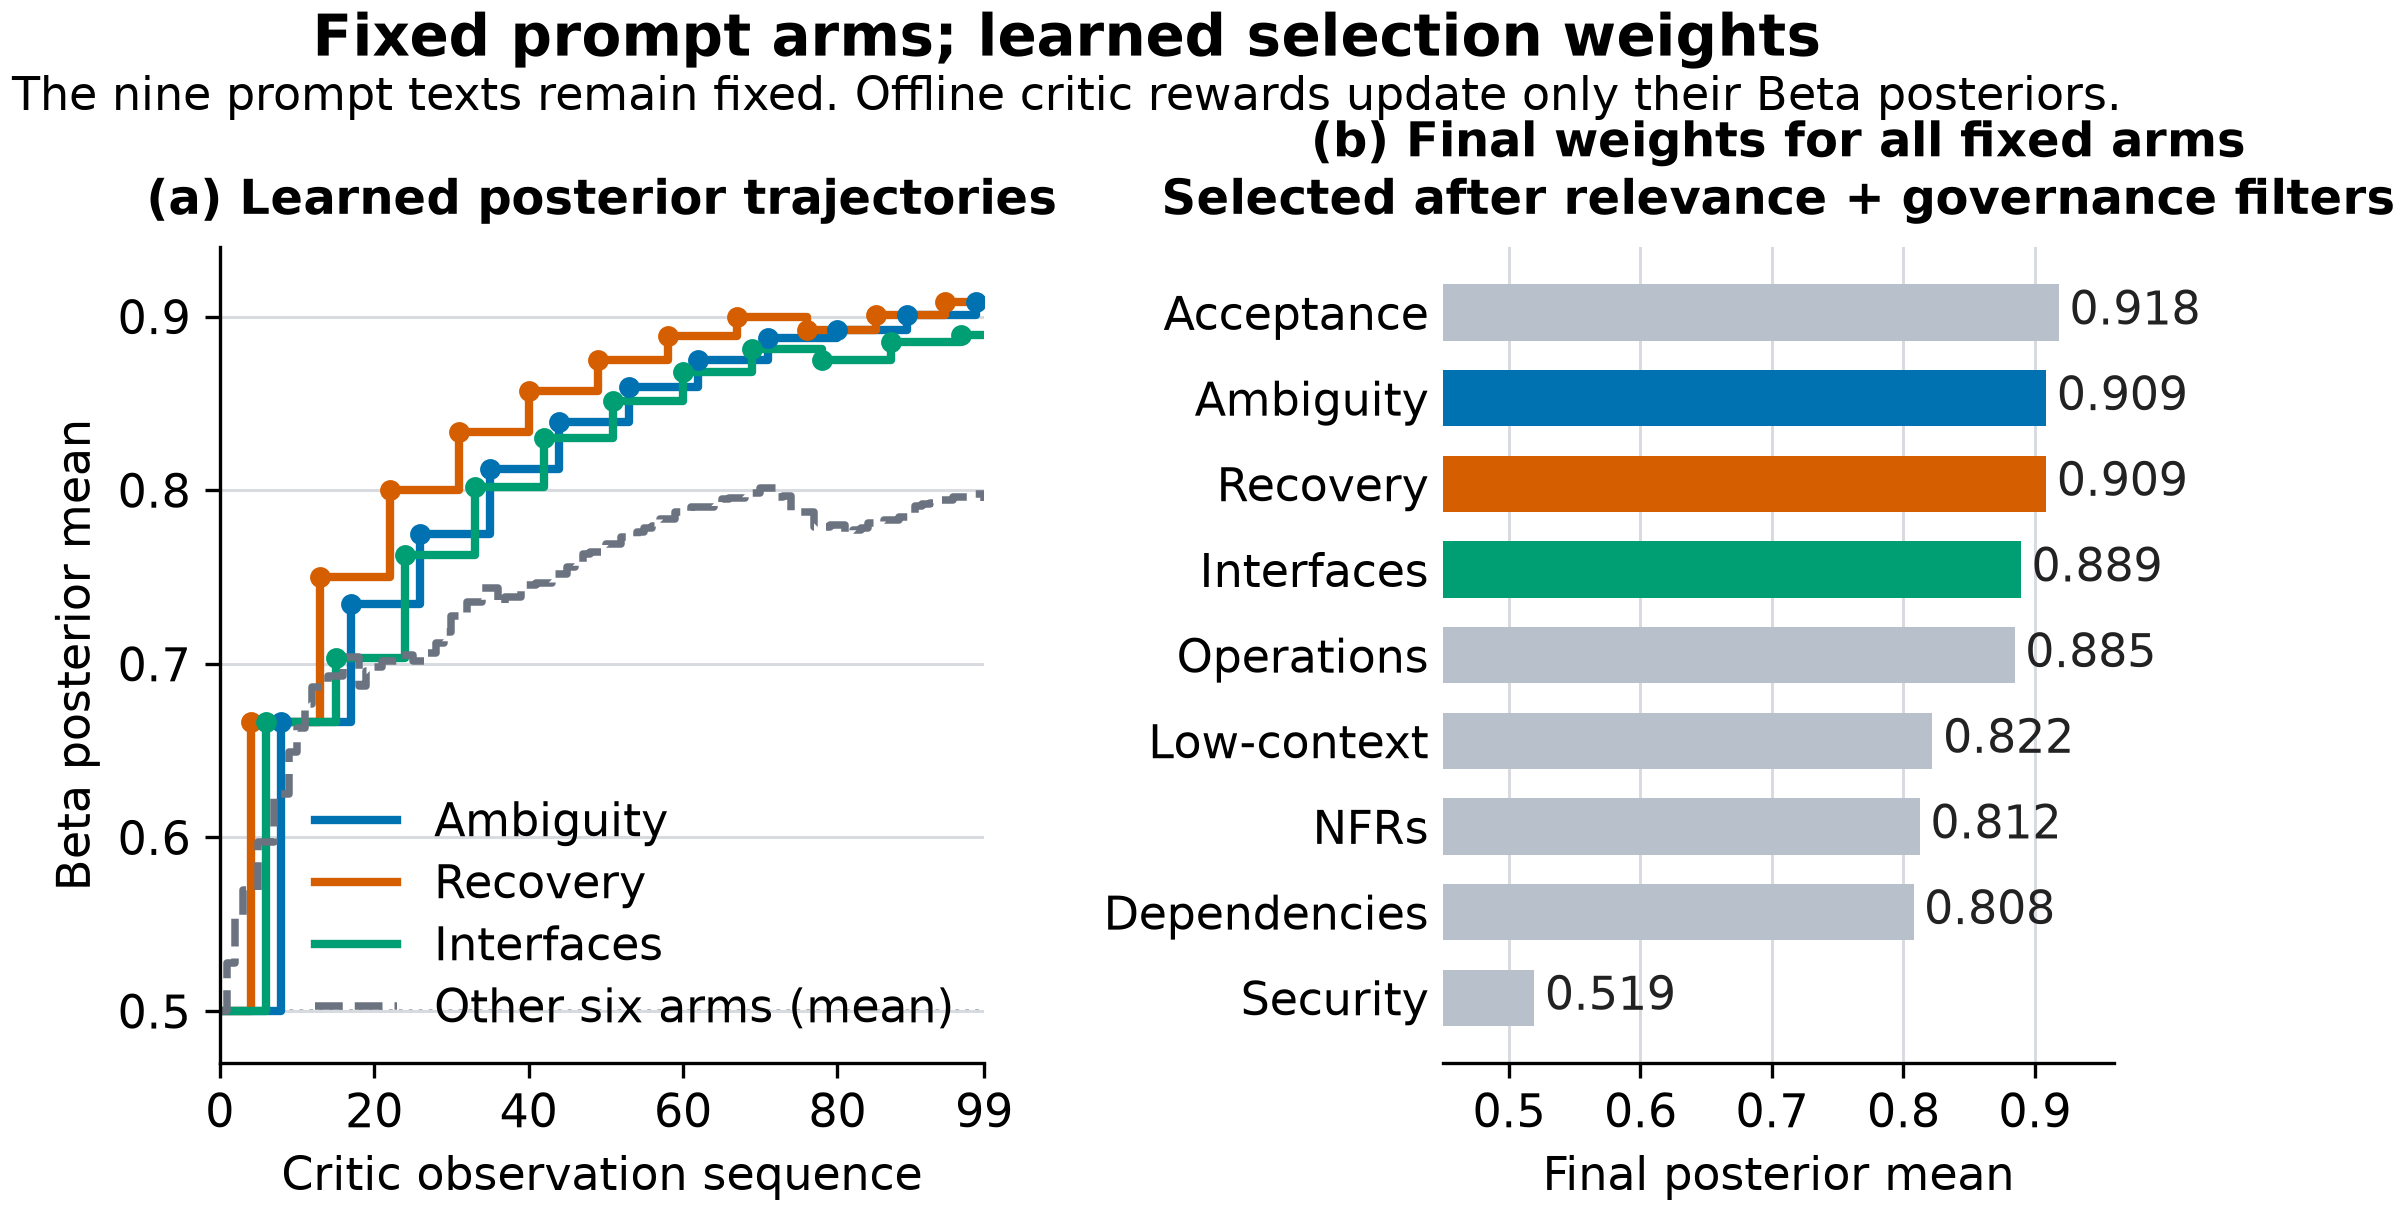
\includegraphics[width=0.97\textwidth]{generated/b2_b3_arm_learning.png}
\caption{Learning trace for nine bounded prompt-policy arms in the held-out diagnostic. Panel (a) depicts posterior means of the 99 critic records archived. Three colored lines depict the arms which were selected during exploitation. The gray line depicts the remaining six arms. Panel (b) demonstrates the posterior means of each arm after 11 observations. The held-out packets were not used for learning. The curve describes posterior learning; it is not a curve of human-rated quality or delivery performance.}
\Description{A two-panel learning figure. The left panel shows posterior means across 99 critic observations for the three arms selected during held-out exploitation and the mean of the other arms. The right panel shows final posterior means for all nine bounded arms and highlights the three selected arms.}
\label{fig:b2-b3-arm-learning}
\end{figure*}

The held-out set contained three preselected requirements packets. B2 used \texttt{gpt-5.6-sol} at ultra reasoning effort and made one generation pass. B3 also used \texttt{gpt-5.6-sol} at ultra reasoning effort. It made an initial draft and then applied three governed refinement passes. Two model evaluators received the outputs under masked condition labels and scored eight criteria from 0 to 4.

Both evaluators preferred B3 for every held-out packet. Thus, all six evaluator--packet judgments favored B3. B3 scored 187/192 (97.4\%), while B2 scored 148/192 (77.1\%). The observed difference was 39 points, or 20.3 percentage points. B3 also scored higher on every criterion in Table~\ref{tab:b2-b3-heldout-diagnostic}. The evaluators identified no missing source requirement in B3 and 13 in B2. Across both evaluators, B3 received 40 model-evaluator-suggested follow-up prompts, compared with 50 for B2. B3 therefore had higher observed scores and fewer suggested follow-up prompts in this diagnostic.

\begin{table}[t]
\centering
\small
\caption{Criterion totals in the held-out diagnostic. Each criterion has a maximum score of 24 across three packets and two blinded model evaluators.}
\label{tab:b2-b3-heldout-diagnostic}
\begin{tabularx}{\columnwidth}{@{}Xrr@{}}
\toprule
Criterion & B2 & B3 \\
\midrule
Source fidelity & 20 & 23 \\
Story boundaries & 22 & 24 \\
Measurable acceptance & 19 & 24 \\
Dependencies and interfaces & 18 & 24 \\
Failure and recovery & 18 & 22 \\
Non-functional and operations & 16 & 22 \\
Evidence and open questions & 15 & 24 \\
Security and compatibility & 20 & 24 \\
\midrule
Total & 148 & 187 \\
\bottomrule
\end{tabularx}
\end{table}

This diagnostic does not replace the matched human study. It used only three purposively selected packets and two model evaluators. No significance test was performed. B3 was also 67\% longer than B2, and the conditions differed in number of passes. The result therefore applies to the complete tested configurations. It does not show that learned arm selection alone caused the difference. The earlier human comparison remains the main evidence for artifact quality. That comparison found no detectable B3--B2 composite difference. The two evaluations answer different questions and are reported separately.

\FloatBarrier
\subsection{Controlled Mutation-Safety Fault Injection (RQ3)}

\noindent\textit{RQ3: What failure modes emerge when agentic planning systems interact with enterprise issue trackers, including missing evidence, duplicate story creation, partial writeback failure, and stale approvals?}\par

We tested the writeback boundary independently of text generation. The experiment applies the same payload and fault schedule to four arrangements: A0 ordinary approval plus logging; A1 source-hash conditional write; A2 source hash plus atomic idempotency; and A3 a source-bound transaction envelope that additionally binds source revision, approved draft version and hash, policy snapshot, reviewer decision, and target set. The nine scenarios are valid control, source edit, source ABA, draft drift, policy drift, target drift, response-loss retry, concurrent retry, and combined source/draft drift. Each scenario contains 2,000 distinct payloads, giving 18,000 transactions for each arrangement and 72,000 method-level observations in total.

\FloatBarrier
\begin{table*}[t]
\centering
\small
\caption{Controlled mutation-safety ablation. Rates use an equal mixture of the nine declared scenarios and therefore measure coverage under the injected schedule, not production prevalence. Eligible-write success is computed over valid-control and retry scenarios.}
\label{tab:mutation-safety-ablation}
\begin{tabularx}{\textwidth}{@{}Xrrrrr@{}}
\toprule
Arrangement & Stale mutation & Duplicate mutation & Any unsafe mutation & Correct outcome & Eligible-write success \\
\midrule
A0 ordinary approval/log & 66.7\% & 33.3\% & 88.9\% & 11.1\% & 33.3\% \\
A1 source-hash conditional & 44.4\% & 22.2\% & 66.7\% & 33.3\% & 33.3\% \\
A2 source hash + atomic idempotency & 44.4\% & 0.0\% & 44.4\% & 55.6\% & 100.0\% \\
A3 source-bound transaction envelope & 0.0\% & 0.0\% & 0.0\% & 100.0\% & 100.0\% \\
\bottomrule
\end{tabularx}
\end{table*}

A3 blocked every injected stale mutation and condensed retry duplicates into a single remote mutation while preserving every eligible write. Comparison with A2 highlights the impact of linking approval with factors other than the current status of the source. Using the hash of only the source does not help in detecting ABA modifications, generation of new drafts, changes in policy, or changes in the target set, in case there is no change in the Jira text. Seven test cases illustrate proper envelope construction, protection against stale approvals, and allowing of idempotence. These test cases highlight how the protection of stale approvals and idempotence happens considering the fault model defined. The frequency and the impact of these measures are not evaluated as part of the production usage.

In Figure~\ref{fig:confidence-composite-combined}(a), the trace of arm learning from the most recent archive is used. There are 99 critic observations from 11 packets that are not held out. The nine different bound strategies have been tested on each of these packets. The heatmap provides information about the reward for each strategy--packet combination. The held-out packets were excluded from learning.

This panel exposes the learning signal behind the posterior curves in Figure~\ref{fig:b2-b3-arm-learning}. It is an offline model-critic diagnostic. It is not live attempt telemetry, a human quality rating, or evidence of delivery performance. The posterior trace and held-out selection log are kept separate to avoid training--evaluation leakage.

Overall, the live block demonstrates that the authenticated workflow is feasible and gives the pairs of endpoint telemetry.

\FloatBarrier
\section{Generalizability Boundaries and Workflow Trade-offs}

\subsection{Simulation-Based Comparative Sensitivity Analysis (B0--B3)}

The B0--B3 block represents a deterministic stress test of the design space rather than four executions of the observed method. B0 generates a formulaic reference. B1 uses lexical rules and fixed metric equations. B2 analyzes the issue text and generates a generic-LLM-style profile using fixed heuristics, without calling a language model. B3 uses the observed Jira Enhancer confidence and readiness as anchor values, whereas its coverage, time, edit, rework, and governance values are computed from declared formulas. Each row indicates the run-item and intermediate features used by each core.

This diagnostic block checks whether the scoring and composite-index models remain stable when the observed runtime units are perturbed in a controlled fashion. It allows sensitivity analysis, mechanism analysis, and implementation regression testing. Nevertheless, it cannot measure the performance of manual teams or generic LLMs, nor it can evaluate the causal effect of Jira Enhancer on that performance \cite{R55}. The matching experiment mentioned above gives the independently executed B1, B2, and B3 artifacts required to answer RQ4; the produced profiles are still different from the observed null B3--B2 quality contrast.

Figure~\ref{fig:confidence-composite-combined} contains two compact diagnostics next to each other while keeping their different evidentiary value. Figure~(a) is the archive of the model-critic reward chart, while Figure~(b) is the sensitivity chart obtained through the formulas.

\begin{figure*}[t]
\centering
\begin{subfigure}[t]{0.485\textwidth}
\centering
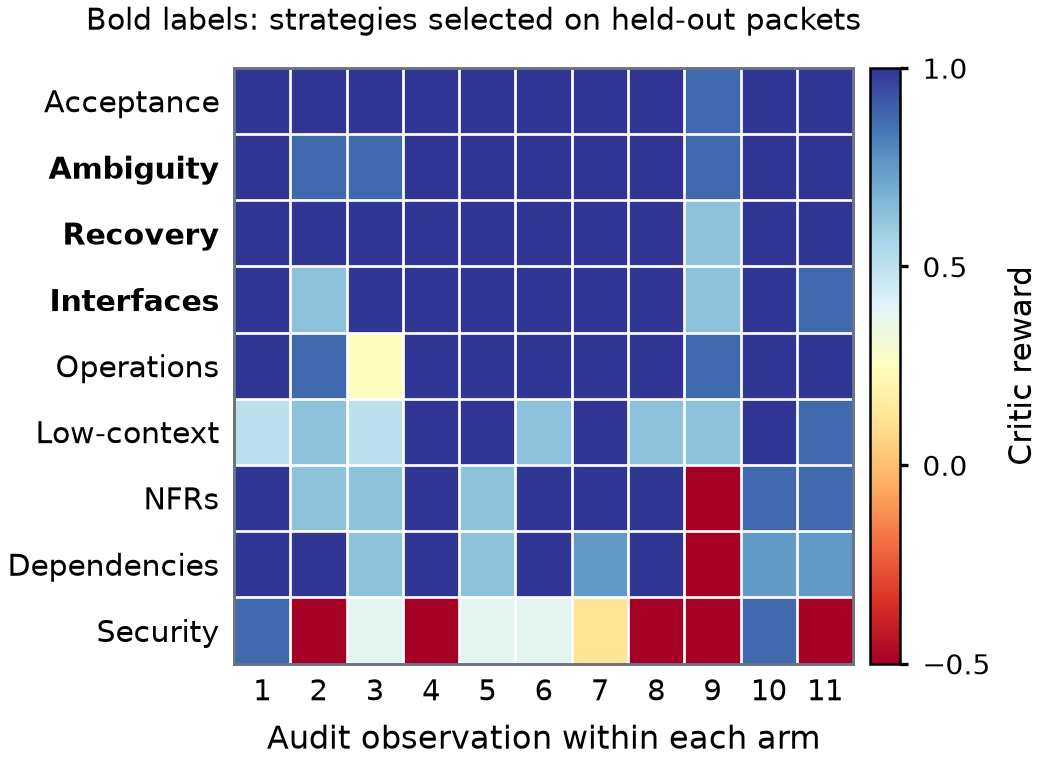
\includegraphics[width=\linewidth]{generated/b2_b3_critic_reward_heatmap.png}
\caption{Recorded critic rewards by strategy.}
\label{fig:b2-b3-critic-rewards}
\end{subfigure}\hfill
\begin{subfigure}[t]{0.485\textwidth}
\centering
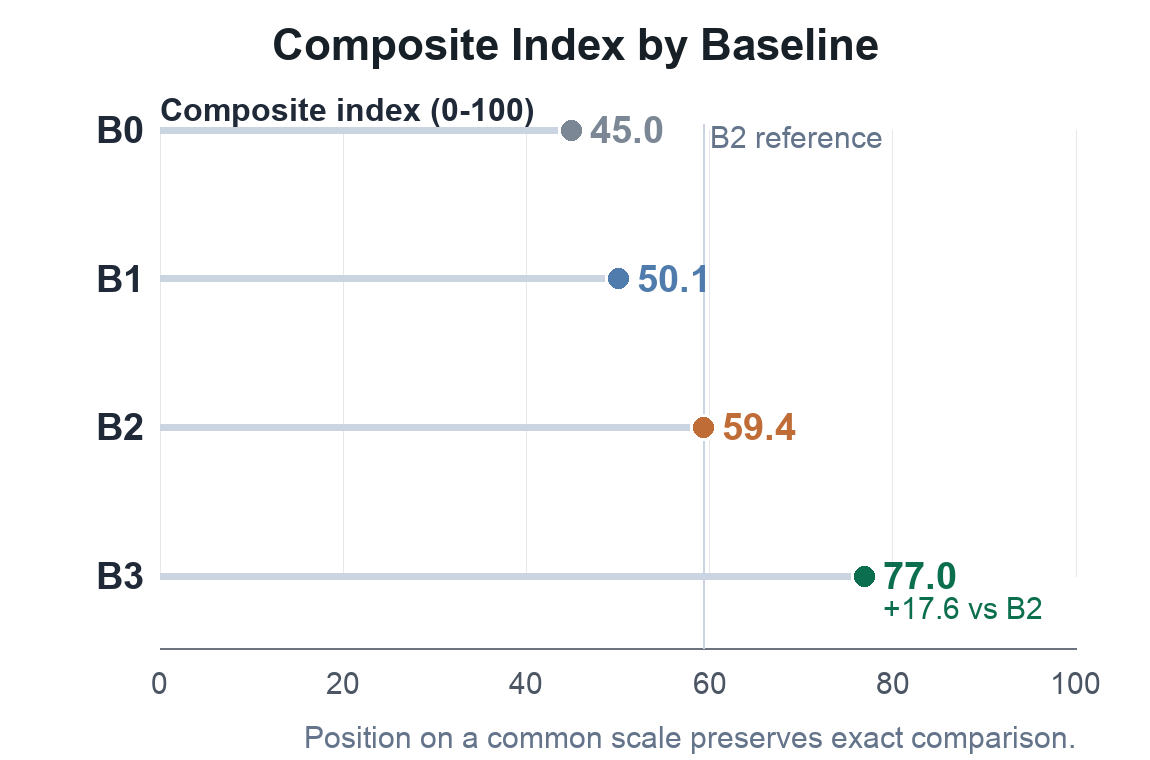
\includegraphics[width=\linewidth]{generated/comparative_composite.png}
\caption{Scoring-model composite profile.}
\label{fig:comparative-composite}
\end{subfigure}
\caption{Diagnostics with different evidence status. Panel (a) shows all 99 rewards from the offline model-critic audit. It contains 11 non-held-out observations for each of nine bounded strategies. Bold labels mark the strategies later selected for held-out refinement. Panel (b) compares composite indices in the formula-generated sensitivity model. B0 is the equation-based manual reference, B1 is the lexical template/rule core, B2 is the generic-LLM-style heuristic core that does not use an LLM, and B3 is the equation-based profile informed by the observed Jira Enhancer confidence and readiness.}
\Description{Two side-by-side charts. Panel (a) is a heatmap of 99 critic rewards arranged by bounded strategy and non-held-out audit observation. Panel (b) is a radial bar chart comparing scoring-model composite index values for B0, B1, B2, and B3.}
\label{fig:confidence-composite-combined}
\end{figure*}

The formulas defined in Figure~\ref{fig:confidence-composite-combined}(b) yield composite mean scores of B0=44.96, B1=50.06, B2=59.38, and B3=76.96. In the model, the B3 profile outperforms the B2 profile by 17.58 points. The difference between the two is explained by the model assumptions and weights and not by the lift over the executed LLM baseline.

\subsection{Observed B3 Advantages Beyond Artifact Score}

B2 is the control of text generation in one run. On top of B2, B3 has added evidence packing, bounded refinement, confidence scoring, policy evaluation, audit persistence, approval binding, recovery state, and conflict-safe writeback. These mechanisms are not considered in the matched artifact score. They thus do not represent the entire workflow in themselves.

The human study presents definite evidence that B3 outperforms B1. In terms of matched epics, B3 performed better than B1 in all 14 instances. B3 exceeded B1 by 1.56 composite points. The comparison with B2 is more detailed. The recorded mean assessment time was 1.02 minutes lower for B3 than for B2 (Holm-adjusted exact \(p=0.0098\), paired rank-biserial \(r_{rb}=-0.78\)). Ready-or-Minor-revision ratings were 88.1\% for B3 and 66.7\% for B2. Major revision decisions for B3 were 5, but for B2, they were 14. But the composite difference for artifact only was not significant.

The later held-out diagnostic adds a different result. The learned-selection B3 configuration scored 187/192, compared with 148/192 for one-shot B2. All six paired model judgments favored B3. B3 therefore had higher observed scores in this diagnostic. This is not a causal estimate of the learned-selection effect, because the refinement budgets also differed.

The workflow conclusion also uses mechanism and fault evidence. Table~\ref{tab:failure-mode-coverage} lists controls that are present in B3 and absent from B2. Table~\ref{tab:mutation-safety-ablation} reports zero unsafe mutations and 100\% eligible-write success for B3's source-bound transaction mechanism. B0 has not been executed on the matched inputs. Its lower value appears only in the scoring-model stress test. Therefore, no measured B3--B0 superiority claim is made. Across the executed evidence, B3 combines lower recorded review burden with learned, governance-filtered prompt-arm selection, recovery, and fault-tested mutation controls.

\begin{table*}[t]
\centering
\small
\caption{Comparison of failure-mode coverage. This table presents a mechanism-oriented analysis derived from implemented behavior, not a measured frequency table. It identifies the collaboration failures explicitly represented and recoverable in each approach.}
\label{tab:failure-mode-coverage}
\begin{tabularx}{\textwidth}{@{}p{0.22\textwidth}p{0.18\textwidth}p{0.18\textwidth}p{0.18\textwidth}X@{}}
\toprule
Failure mode & B0 manual & B1 template/rule & B2 generic LLM & B3 Jira Enhancer \\
\midrule
Missing external evidence & Manual delay or meeting follow-up & No evidence-aware handling & Risk of fluent but weakly grounded output & Warning codes plus embedded Jira-context fallback when substantive design text exists \\
Duplicate story creation & Depends on reviewer memory & Weak summary matching only & Possible if generated wording changes & Deterministic normalized-summary skip with existing issue key reported \\
Partial create failure & Manual reconciliation & No preserved decision state & No structured partial outcome & Per-story \texttt{create\_failed} status, skipped list, and retry-preserved UI state \\
Stale approval after tracked edit & Human process risk & Not modeled & Not modeled & Source-hash check blocks writeback and forces revalidation \\
Unsafe high-confidence output & Reviewer judgment only & Static guardrails & Confidence may be uncalibrated & Confidence threshold, validation, policy gate, and explicit approval key \\
\bottomrule
\end{tabularx}
\end{table*}

Table~\ref{tab:failure-mode-coverage} captures the implemented mechanism-coverage model. It is not a frequency distribution; the controlled fault-injection experiment in Table~\ref{tab:mutation-safety-ablation} provides evidence for RQ3.

\subsection{Mechanisms Encoded in the B3 Profile}
The generated B3 profile, thus, involves a stacked set of mechanisms instead of making a single prompt choice:
\begin{enumerate}
  \item \textbf{Critic loop driven by rubrics with threshold criteria:} candidate drafts get iteratively revised until the target thresholds of clarity, testability, dependency, evidentiary basis, and actionability are achieved.
  \item \textbf{Context packing instead of evidence passthrough:} the model gets compressed and prioritized context on policy issues instead of massive and noisy evidence input.
  \item \textbf{Checks for contradictions and gaps before policy evaluation} ensure that only safe and fluent output is marked as ready.
  \item \textbf{Governance-aware scoring:} lack of consistency or low rubric ratings lower confidence and readiness scores.
  \item \textbf{External mutation control by the policy:} even a draft candidate with a high readiness score must be evaluated and approved to undergo an external mutation.
\end{enumerate}
The above mechanisms are the foundations of the B3 scoring assumptions and are part of the implementation; however, the generated comparison will not be able to detect them as separate sources of the difference modeled in B3. Measured ablation will turn off each mechanism individually on the same set of inputs, starting with the critic loop, context packing, validator, and policy coupling. Thematic background and Table~\ref{tab:related-work-comparative} link findings from the domains of retrieval, reasoning, tool orchestration, and governance to the B3 mechanisms.

\FloatBarrier
\subsection{Generated-Unit Stress Test (5{,}000 Units)}
The stress test of the generator is performed by subjecting the generator to runtime units based on deterministically seeded perturbations such that 5{,}000 units are generated after which B0--B3 score formulas are tested using the generated units. The generated dataset has item-level features, summary statistics, and high-lift cases but doesn't generate 5{,}000 independent epics.

The method-level composite distributions are:
\begin{itemize}
  \item \textbf{B0 manual:} mean 44.96, std 1.05.
  \item \textbf{B1 template rules:} mean 50.06, std 1.07.
  \item \textbf{B2 generic LLM:} mean 59.38, std 0.72.
  \item \textbf{B3 Jira Enhancer:} mean 76.96, std 1.22.
\end{itemize}
For each method $m$ (\(n=5{,}000\) units per method), the composite index is calculated as follows:
\begin{equation}
\mathrm{Composite}_m
= w_Q Q_m + w_{\mathrm{Eff}}\mathrm{Eff}_m + w_G G_m,\qquad
w_Q+w_{\mathrm{Eff}}+w_G=1,\; w_Q,w_{\mathrm{Eff}},w_G\ge 0.
\end{equation}
Equal weights are applied to all the four generated profiles. Figure~\ref{fig:performance-raincloud-combined}(b) shows an efficient raincloud representation of the generated scores. Figures~\ref{fig:comparative-5000-violin} and~\ref{fig:comparative-5000-components} give two diagnostic views of the scores. The two figures answer different questions regarding the scoring formulas.

The violin plot in Figure~\ref{fig:comparative-5000-violin} depicts the distribution of each generated distribution. The median and interquartile range are 44.95 [44.26, 45.69] for B0, 50.45 [49.04, 50.89] for B1, 59.33 [59.09, 59.69] for B2, and 77.27 [75.83, 78.05] for B3. The narrow distributions show that the seeded perturbations maintain the separation contained within the formulas.

In Figure~\ref{fig:comparative-5000-components}, the composite index is decomposed into quality, efficiency, and governance. Since all methods use the same 0--100 axis, the components can be directly compared. The generated B2 profile generates 73.76, 52.33, and 41.97 in these dimensions. The generated B3 profile records 88.18, 66.97, and 68.76. The largest modeled gap is in governance. This result explains how the declared B3 formula produces a higher composite score. 

The generated time-to-ready values provide an additional sensitivity check. The mean values for B0--B3 are 187.88, 130.04, 115.37, and 74.49 minutes. The corresponding P90 values are 193.14, 135.96, 117.28, and 77.11 minutes. 

\begin{figure*}[tbp]
\centering
\begin{subfigure}[t]{0.485\textwidth}
\centering
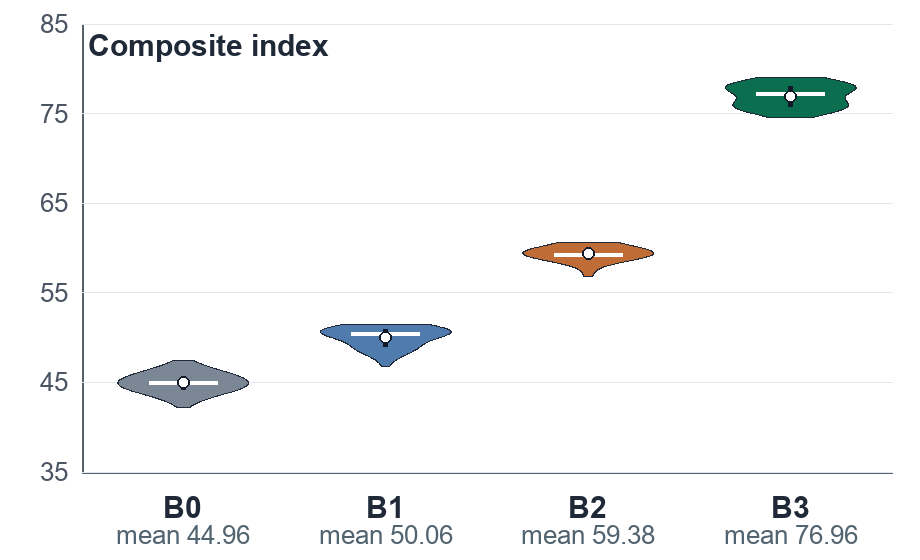
\includegraphics[width=\linewidth]{generated/comparative_5000_violin_main.png}
\caption{Composite density and spread.}
\label{fig:comparative-5000-violin}
\end{subfigure}\hfill
\begin{subfigure}[t]{0.485\textwidth}
\centering
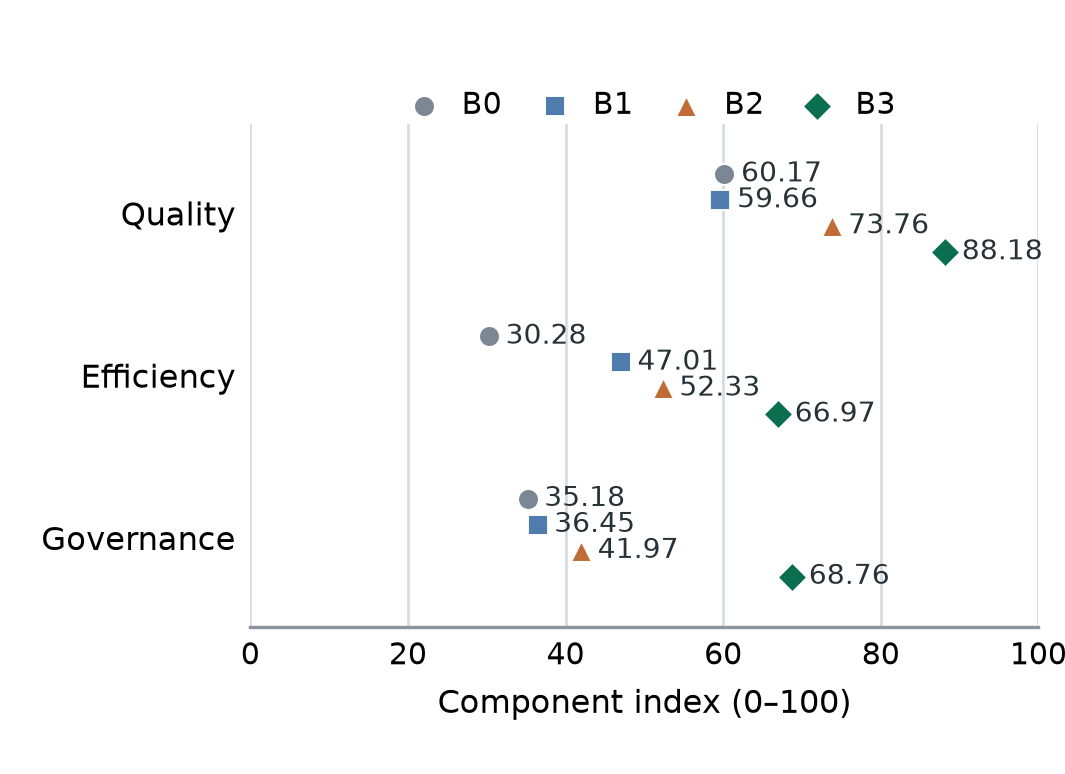
\includegraphics[width=\linewidth]{generated/comparative_5000_component_profile_main.png}
\caption{Component indices on a common scale.}
\label{fig:comparative-5000-components}
\end{subfigure}
\caption{Two diagnostics from the 5,000-unit stress test. Panel (a) shows density, interquartile range, median, and mean. Panel (b) shows the mean component indices. Both panels audit the scoring model. They do not report observed comparative performance.}
\Description{A two-panel figure containing a violin plot and a horizontal component-profile dot plot. Both panels compare the B0, B1, B2, and B3 scoring profiles.}
\label{fig:comparative-5000-diagnostics}
\end{figure*}

Both panels audit deterministic outputs of the declared formulas. The 5,000 rows per profile are seeded perturbations of reused runtime-derived units. They are not 5,000 independent epics or executed treatments. The plots also do not replace the blinded matched comparison. In that comparison, the B3--B2 package-score difference was 0.10 points, with a 95\% confidence interval of $[-0.13,0.36]$ and a Holm-adjusted $p$-value of 0.485.

\FloatBarrier

\subsection{Public Issue-Text Sensitivity Check (SWE-bench Lite)}

Using the SWE-bench Lite public test split (\(n=300\)) \cite{R26}, the analysis extracts problem text, hints, and test identifiers; derives lexical complexity, confidence, and readiness features; and applies the same B0--B3 formulas. It does not ask any method to generate a patch, execute repository tests, or measure issue resolution. The following tables are therefore a public issue-text transfer check for the scoring generator, not SWE-bench performance results.

\begin{table*}[t]
\centering
\small
\caption{Cross-input sensitivity comparison of the internal generated units and 300 SWE-bench Lite issue texts. \(\Delta\) to B3 is calculated from formula-derived composite values within each input set.}
\label{tab:cross-dataset-comparative}
\resizebox{\textwidth}{!}{\begin{tabular}{llrrrrrr}
\hline
Dataset & Method & N & Quality & Efficiency & Governance & Composite & $\Delta$ to B3 \\
\hline
Internal 5,000-unit run & B0 & 5000 & 60.17 & 30.28 & 35.18 & 44.96 & +32.01 \\
Internal 5,000-unit run & B1 & 5000 & 59.66 & 47.01 & 36.45 & 50.06 & +26.90 \\
Internal 5,000-unit run & B2 & 5000 & 73.76 & 52.33 & 41.97 & 59.38 & +17.58 \\
Internal 5,000-unit run & B3 & 5000 & 88.18 & 66.97 & 68.76 & 76.96 & +0.00 \\
SWE-bench Lite test & B0 & 300 & 60.39 & 30.62 & 35.21 & 45.16 & +32.73 \\
SWE-bench Lite test & B1 & 300 & 57.72 & 48.20 & 35.34 & 49.27 & +28.62 \\
SWE-bench Lite test & B2 & 300 & 79.36 & 48.39 & 42.79 & 60.93 & +16.96 \\
SWE-bench Lite test & B3 & 300 & 89.92 & 66.65 & 69.72 & 77.89 & +0.00 \\
\hline
\end{tabular}
}
\end{table*}

Table~\ref{tab:cross-dataset-comparative} shows that the formulas produce the same ranking on both input sets, with B3 \(>\) B2 \(>\) B1 \(>\) B0. Formula-derived B3--B2 differences are +17.58 internally and +16.96 on public issue text. This agreement indicates stability of the scoring assumptions under a change in text source; it does not demonstrate cross-dataset method effectiveness.

\begin{figure*}[t]
\centering
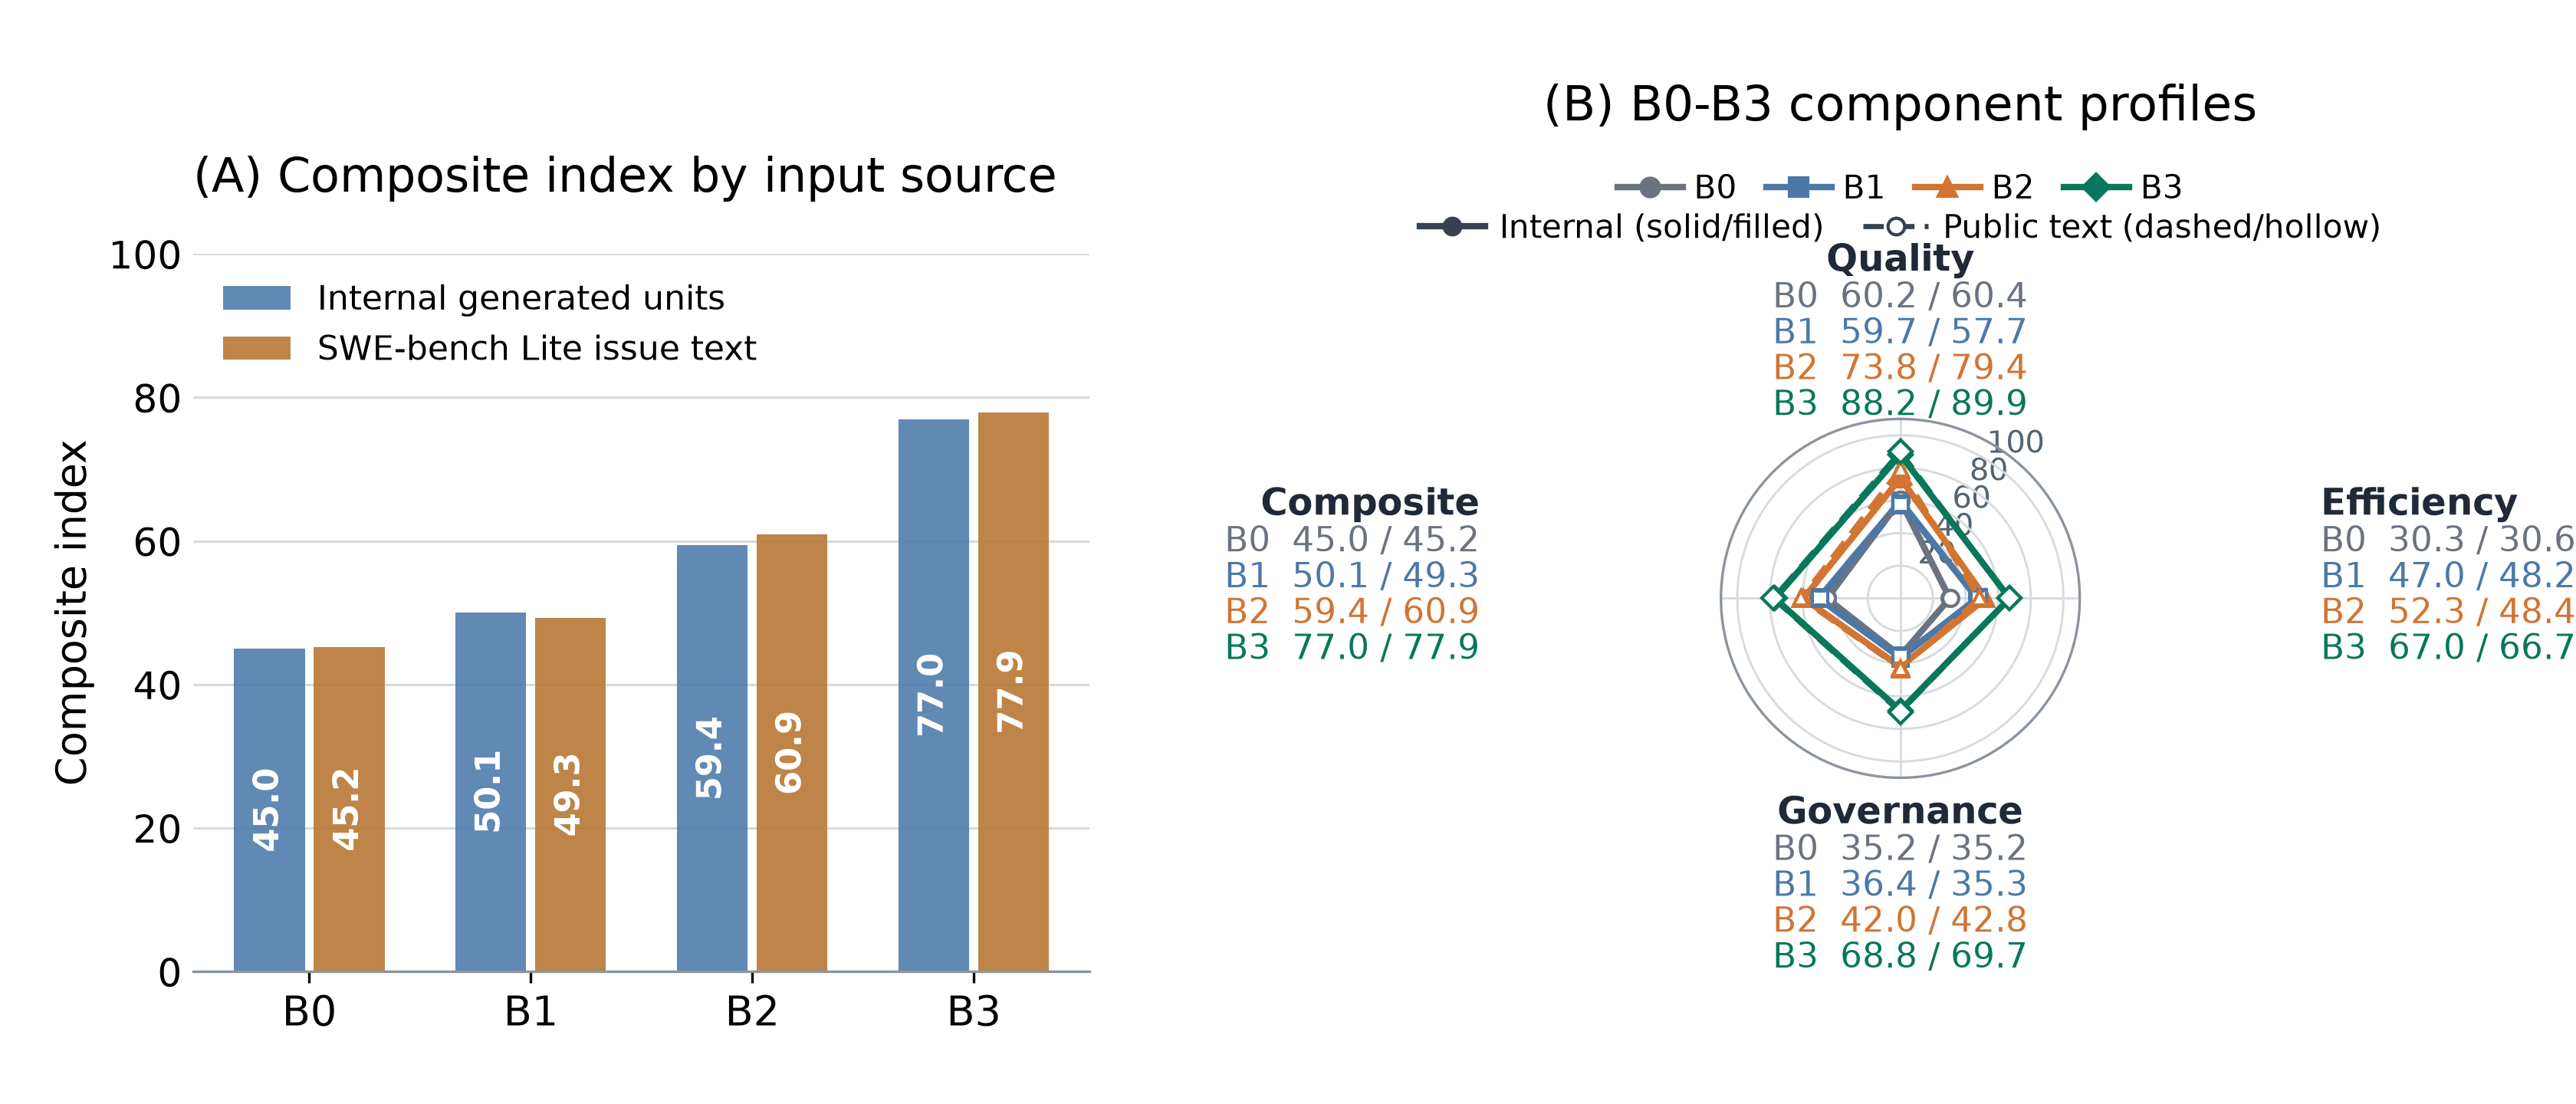
\includegraphics[width=0.94\textwidth]{generated/comparative_cross_dataset_multiplot.png}
\caption{Cross-input sensitivity view. Panel (A) reports scoring-model B0--B3 composite indices for internal generated units and public issue text. Panel (B) overlays the corresponding B0--B3 component profiles on a 0--100 radar scale. Each numeric pair is reported as internal/public issue text. No patches or benchmark tests are executed.}
\Description{Two-panel chart. Panel A uses grouped bars to compare B0--B3 composite indices for internal generated units and SWE-bench Lite issue text. Panel B uses a radar plot to compare B0--B3 quality, efficiency, governance, and composite indices. Clear labels around the radar show each internal and public value pair.}
\label{fig:cross-dataset-comparative}
\end{figure*}

Figure~\ref{fig:cross-dataset-comparative} shows the same scoring-model behavior in two forms. The radar profiles include all four methods, keep the same B3--B2 pattern across the four indices, and display each value directly. This is a sensitivity result, not a cross-dataset effectiveness test.

\begin{table}[t]
\centering
\small
\caption{Formula-derived SWE-bench Lite issue-text sensitivity results: all-method profiles and the B2--B3 difference. These values are scoring-model outputs.}
\label{tab:public-benchmark-results}
\label{tab:public-benchmark-method-summary}
\label{tab:public-benchmark-before-after}
\textbf{Panel A: All-method profile summary}\par\smallskip
\resizebox{\columnwidth}{!}{\begin{tabular}{lrrrrr}
\hline
Method & Quality & Efficiency & Governance & Composite & Time-to-ready (min) \\
\hline
B0 & 60.39 & 30.62 & 35.21 & 45.16 & 187.03 \\
B1 & 57.72 & 48.20 & 35.34 & 49.27 & 122.78 \\
B2 & 79.36 & 48.39 & 42.79 & 60.93 & 139.62 \\
B3 & 89.92 & 66.65 & 69.72 & 77.89 & 74.63 \\
\hline
\end{tabular}
}

\vspace{0.35em}
\textbf{Panel B: B2--B3 difference}\par\smallskip
\resizebox{\columnwidth}{!}{\begin{tabular}{lrrrr}
\toprule
Comparison & Before mean & After mean & Absolute gain & Relative gain (\%)\\
\midrule
B2 $\rightarrow$ B3 on SWE-bench Lite & 60.93 & 77.89 & 16.96 & 27.84\\
\bottomrule
\end{tabular}}

\end{table}

The scoring model assigns mean composites of 60.93 to B2 and 77.89 to B3, a difference of +16.96 points (27.84\% relative to B2). This is a sensitivity delta, not a measured before/after improvement.



\subsection{Artifact and Confidentiality Boundary}

The review artifact retains deterministic analysis scripts, de-identified telemetry for the 70 story endpoints, a de-identified audit of the latest-wave payloads, coded ratings from both artifact assessments, aggregate matched-test tables, fault-injection trial records, seeds, and checksums. The shareable data exclude issue and epic keys, internal URLs, account names, email addresses, and timestamps. Raw Jira and Confluence records, the sanitized matched-input packets, and the private method-allocation key remain access-controlled because the source requirements are confidential enterprise material. We did not collect reviewer names, demographic variables, sensitive attributes, or other personal identifiers. The study also does not measure trust, workload, satisfaction, or individual performance.

\FloatBarrier
\section{Discussion: Post-Evaluation Analysis}

\subsection{Reliability and Error Handling}

The system classifies warning codes, such as external authentication requirements and MCP unavailability, and propagates them to run- and story-level review records. This supports graceful degradation:
\begin{equation}
\texttt{service\_mode} \in \{\texttt{full-context},\texttt{reduced-context}\}.
\end{equation}
\textit{Full-context} mode is used for cases with external evidence; \textit{reduced-context} mode is applied when only issue-local evidence is available.

\textit{Reduced-context} mode is designed to remain useful instead of failing softly. It still provides structured drafts and warning metadata, which allows reviews to continue in an informed way.

In reliability engineering, the ``graceful capability collapse'' pattern is applied instead of binary failure. For example, if a high-value evidence source such as Confluence is offline, the system retains decomposition capability by using the available issue records and marking the missing evidence categories. Available issue records prevent planning deadlock, while metadata preservation maintains the meaning of the confidence score.

Transient failures are retried using exponential backoff and jitter, while terminal errors are reported with machine-actionable error codes. The technique allows for automatic retry management at the orchestration layer without hiding permanent integration issues.

The user-guided workflow maintains collaboration context through the stages in case of failures. If the story creation fails or times out, then the selected stories will still be present in the console. User will be able to look at the partial generation results in Jira and continue working on them without having to regenerate the decision set. Such capability is important for human--AI cooperation since recovery should not be limited to backend functionality but should be visible for a human making retry, change, or cancel decisions.

\subsection{Positioning and Novelty Scope}

Evidence blocks can validate various claims: 70 authenticated endpoints show that a successful path is feasible; independent ratings were provided for 69 full-text stories and 14 epic packages; five experts compared 42 B1, B2, and B3 packages together with 210 stories; fault injection shows safety of writeback; 5{,}000-unit and public issue text blocks show declared numerical behavior. The study does not measure cross-project and longitudinal delivery benefits, which remain important in light of unreliability, human values, and unavailability of standardized evaluation of AI in software engineering \cite{R59,R81,R60}.

Learned prompt-arm selection is another part of B3's novelty. B3 does not use an unrestricted prompt loop. It organizes refinement strategies as versioned, bounded policy arms. At runtime, the selected strategy is combined with the current evidence, gap signals, confidence, and attempt state. A contextual bandit selects only from arms that pass the governance checks \cite{R84,R86}. Learning updates the Beta posterior used for later selection. The selected arm, refinement result, and posterior update are recorded for auditing, as shown in Table~\ref{tab:policy-arms} and Algorithm~\ref{alg:rl-policy-update}. This design supports adaptive selection without giving the learning layer permission to modify Jira. Final mutation still requires validation, policy checks, and human approval.

The matched experiment evaluated B3 with a frozen pre-study policy. It did not isolate the RL component. The later diagnostic recorded a separate learning trace. It used 99 critic observations from 11 non-held-out packets and excluded the three evaluation packets. Figure~\ref{fig:b2-b3-arm-learning} shows how the posterior means evolved. The diagnostic then used governance-filtered, zero-exploration selection on the held-out packets. This result demonstrates that the complete learned-selection configuration can be tested and audited. It still does not show that learning alone caused the observed B3--B2 difference.

B3 controls learning, confidence, governance, approval, recovery, and conflict-free writeback. The score of B3's blinded artifact did not differ significantly from B2's, but B3 took less assessment time, had a descriptively better revision profile, and was the only one that could proceed through a source-bound mutation pathway tested under stale state, retry, draft drift, policy drift, and target drift. This evidence supports the bounded advantage of end-to-end workflows.

\section{Lessons Learned}

The study produced six practical lessons. Each lesson is limited to the evidence that supports it.

\begin{enumerate}
  \item \textbf{Different evaluations answer different questions.} The study uses four types of evidence, as summarized in Table~\ref{tab:evidence-hierarchy}. First, the field trace contains 70 verified end states. These include 69 newly created Jira issues and one safe-duplicate resolution. The latest wave also includes 44 audited new payloads. Second, human reviewers assessed artifact quality. Two reviewers assessed 69 full-text stories and 14 epic packages. Five reviewers compared 42 matched B1, B2, and B3 packages containing 210 stories. Third, the fault-injection experiment tested mutation safety across 72,000 scenario-balanced observations. Finally, formula-based sensitivity analyses remain diagnostic evidence. These evaluations have different goals and units. Therefore, their results are reported separately and are not combined into one overall result.

  \item \textbf{B3 automates refinement that B2 leaves outside the pipeline.} B2 generated one generic version per epic and then terminated. There was no critic step, confidence feedback, retry process, or prompt policy choice. Further refinement needed human guidance or another controller. B3 employed a bounded critic loop with learned, governance-filtered prompt arm selection. In the parallel experiment, the average assessment time was 1.02 minutes shorter with B3. The reviewers made 5 Major revision choices for B3 and 14 for B2. The total artifact score difference was not statistically significant. In the subsequent held-out diagnostic test, the model assessors proposed 40 further prompts for B3 and 50 for B2. They also preferred B3 on all six comparison judgments. These data favor automatic, governed refinement with less follow-up. They do not indicate better prose or reduced compute cost overall. Human judgment is required for omitted domain choices and final approval.

  \item \textbf{Human approval requires a technical limit.} Simply approving the draft cannot prevent the mutation from being stale or redundant. The approved draft must stay tied to the source state that was reviewed by the human. This is accomplished through the source-tied transaction envelope. During the fault injection experiment, it prevented all injected dangerous mutations and permitted all legitimate writes, as noted in Table~\ref{tab:mutation-safety-ablation}. Human power is greater when the writeback contract enforces the approval decision.

  \item \textbf{Missing evidence must be made known.} The system can proceed in reduced context when there is no external evidence. It cannot hide the lack of source evidence. The warning codes and confidence provenance will assist the human in understanding this problem. The draft can still be valuable without being complete evidence.

  \item \textbf{The recovery process should maintain human control.} The generation and write-back procedures can fail at any stage. The workflow should enable the reviewer to continue, try again, or cancel. Regeneration without human interaction would compromise control and auditing.

  \item \textbf{Adaptive models require full trajectories and cost proof.} The live data have the terminal states but not each of the refinement attempts. They cannot prove a complete live learning trajectory. In the latter, there were 99 observations from an offline critic. Those observations revealed how the posterior probabilities evolved but they were model-generated data and not human and delivery outcomes. In comparison to B2, B3 did more model work in both comparisons. Hence faster package assessment does not mean lower cost of computation. Future studies should have each attempt recorded and the outcomes normalized with respect to cost.
\end{enumerate}

Collectively, these lessons lead to a modest conclusion. B3 shows an established path from data to an approved mutation based on the analyzed conditions. The paper does not demonstrate a better prose, delivery quality, productivity, computing efficiency or generalization over different projects.

\section{Implications, Limitations, and Threats to Validity}

\subsection{Future Extensions}

Further research may advance the work of Jira Enhancer in five dimensions. First, multi-objective reinforcement learning can find a trade-off between the confidence level and the cost of models. Second, project velocity will allow story-point estimation. Third, active learning can discover the stories that should be manually verified. Fourth, multilingual prompts will enable the work of the teams using different languages. Finally, dependency graph will link Jira issues, documents, code, and incidents. This graph will help the system to locate the related work and critical paths before decomposition of an epic.

\subsection{Limitations and Validity Threats}
\textbf{Internal validity:} this concerns whether the observed differences come from the evaluated methods rather than the study design. We used the same inputs, neutral formatting, independent randomization, and blinding to reduce bias \cite{R55}. However, the matched workflows were not compute-matched. B2 used 14 model calls, while B3 used 173. For B1, the static completion rule filled slots for 24 of 70 stories. Reviewers~1 and~2 had previously seen B3-only material. We therefore excluded them from the primary analysis. The later held-out diagnostic also compared unequal configurations. B2 used \texttt{gpt-5.6-sol} at ultra reasoning effort and one pass. B3 used \texttt{gpt-5.6-sol} at ultra reasoning effort and three refinement passes after its initial draft. B3 was 67\% longer. The diagnostic therefore cannot isolate the effect of learned selection. The generated-unit analysis also uses formulas rather than executed treatments. It cannot estimate a treatment effect \cite{R71}.

\textbf{Construct validity:} this concerns whether the measures represent the concepts claimed in the study. Confidence is produced and optimized by the same pipeline. It is therefore not an independent measure of quality. Human approval records a workflow decision, not later delivery success. Blinded reviewer ratings measure visible content quality. Recorded assessment time is not total planning time, and the edit counts are estimates. Reviewers could not see the governance metadata. Therefore, the artifact score does not measure policy or writeback value.

\textbf{External validity:} this concerns whether the findings can be applied to other settings. The 70 endpoints come from 14 epics, two deployment waves, and one organization. They represent successful paths only. The data contain no rejected, abandoned, below-threshold, or conflict endpoint. The matched study uses the same portfolio and has no independently authored manual baseline. The learned-selection diagnostic uses only three purposively selected packets and two model evaluators. The public issue-text analysis also does not execute the methods. Claims about transfer therefore require new projects, domains, and practitioners. This is especially important for context-dependent socio-technical tools \cite{R71,R58}.

\textbf{Conclusion validity:} this concerns the strength and precision of the conclusions. The endpoints are nested within epics, the two waves begin with different score distributions, and all terminal decisions succeed. The epic-level exact and cluster-resampled analyses account for this nesting. However, the 14 epic clusters provide limited precision. The B3--B2 interval still permits modest effects in either direction. The ratings showed high inter-rater agreement. The distinct comments indicate that reviewers made independent judgments. However, each reviewer completed only four repetitions. We did not record reviewer experience bands or ask reviewers to guess which method produced each package. The held-out diagnostic has only six paired model judgments and no significance test. Its result is descriptive. The disposition results are also descriptive. The fault-injection rates are scenario-balanced and should not be treated as estimates of production prevalence.

\textbf{Reference currency:} research on human--AI collaboration in software engineering is developing quickly. The related literature should therefore be reviewed and updated periodically \cite{R72}.

\textbf{Mitigation:} future studies should use independently prepared manual packages and compute-matched B2 and B3 configurations. The blinded study should be repeated on new portfolios, and reviewer expertise levels should be recorded. Ablation tests should disable the critic, retrieval, validation, and policy layers one at a time. Future work should also test sensitivity to the selected weights and assess the practical significance of any change. Finally, later studies should observe edits, failures, rework, and cycle-time variation across multiple releases.

\section{Conclusion}


Jira Enhancer is an executable method for governed AI-assisted planning. It converts underspecified epics into reviewable story proposals. It preserves evidence provenance, requires human approval, and protects writeback through source-bound validation and idempotency.

Two authenticated deployment waves show successful-path feasibility. Controlled fault injection validates stale-state and duplicate-mutation protection. The matched human study provides a clear B3 benefit over deterministic B1. The B3 variant scored better on all 14 common epics. Relative to one-time B2, there was no observable performance difference with the artifact composite. But the mean evaluation time was 1.02 minutes lower for B3. It also received 5 Major revision decisions instead of 14 and offered governance and mutation protections that B2 lacked.

B3 was later validated by a held-out diagnostic using a B3 variant with learned governance-filtered prompt-arm selection. B3 scored 187/192, compared with 148/192 for one-shot B2.

Both model evaluators preferred B3 in all three packets. Therefore, B3 had a higher score in the diagnostic. This validation does not single out the role of learning since the refinement passes and output length were also different. From the performed validations, B3 offers a reduced recorded review burden combined with governed refinements and fault-injected mutation protection. It avoids any unsafe mutation while enabling structured refinement and human guidance. This is not a demonstration of overall superiority in prose writing, delivery quality, productivity, or efficiency. Further claims require further validation.

\bibliographystyle{ACM-Reference-Format}
\nocite{R94}
\bibliography{references_2020_plus}

\end{document}
